\documentclass[usenames,dvipsnames,aspectratio=169]{beamer}
%\usepackage{pgfplots}
%\let\textmdorig\textmd
%\let\textscorig\textsc
%\let\textttorig\texttt
%\usepackage{tikz}
%\usetikzlibrary{shapes}
%\usetikzlibrary{arrows}
%\usetikzlibrary{positioning}
%
%
%\renewcommand<>{\textsc}[1]{%
%      \only#2{\textscorig{#1}}%
%  }
\mode<presentation> {
    \usetheme{metropolis}
}
\usefonttheme[onlymath]{serif}
\setbeamertemplate{navigation symbols}{}

\usepackage{lmodern}
\usepackage{booktabs} 
\usepackage{multirow}
\usepackage{colortbl}

\DeclareMathOperator*{\argmin}{arg\,min}

%%%  \usepackage[T1]{fontenc}
%%%  \usepackage{stmaryrd}
%%%  \usepackage{tikz-3dplot}
\usetikzlibrary{calc}

\tikzset{weird fill/.style={append after command={
   \pgfextra
        \draw[sharp corners, fill=#1]% 
    (\tikzlastnode.west)%  
    [rounded corners=3pt] |- (\tikzlastnode.north)% 
    [rounded corners=1pt] -| (\tikzlastnode.east)% 
    [rounded corners=1pt] |- (\tikzlastnode.south)% 
    [rounded corners=3pt] -| (\tikzlastnode.west); 
   \endpgfextra}}}

%%%  \usepackage{dsfont}
%%%  
%%%  \newcommand\T{{\mathpalette\raiseT\intercal}}
%%%  \newcommand\raiseT[2]{\raisebox{0.45ex}{$#1#2$}}
%%%  
%%%  \newcommand{\tikzmark}[1]{\tikz[overlay,remember picture] \node (#1) {};}
%%%  
%%%  \usepackage[normalem]{ulem}
%%%  \usepackage{algpseudocode}
%%%  \usepackage{algorithm}
%%%  %\usepackage{algorithmic}
%%%  \usepackage{graphicx} % Allows including images
%%%  
%%%  \usepackage{xcolor}
%%%  \usepackage{xspace}
%%%  \usepackage{bbm}
%%%  \usepackage{amsfonts}
%%%  \usepackage{amsmath}
%%%  \usepackage{amssymb}
%%%  \usepackage{ulem}
%%%  \usepackage[backend=biber]{biblatex}
%%%  \bibliography{cites.bib}
%%%  
%%%  \newcolumntype{g}{>{\columncolor{black!5}}c}
%%%  \newcolumntype{f}{>{\columncolor{black!5}}r}
%%%  \newcolumntype{L}[1]{>{\columncolor{black!5}}m{#1}}
%%%  \usepackage{tikz}
%%%  \usetikzlibrary{shapes}
%%%  \usetikzlibrary{arrows}
%%%  \usetikzlibrary{positioning}
%%%  \usepackage[most]{tcolorbox}
%%%  
%%%  
%%%  \newenvironment{indentquote}{%
%%%        \par%
%%%          \medskip
%%%            \leftskip=4em\rightskip=2em%
%%%              \noindent\ignorespaces}{%
%%%                    \par\medskip}
%%%  
%%%  \newenvironment{indentquote2}{%
%%%        \par%
%%%          \medskip
%%%            \leftskip=2em\rightskip=2em%
%%%              \noindent\ignorespaces}{%
%%%                    \par\medskip}
%%%  
%%%  
%%%  
%%%  

                  \title[Sal. Est. and Faithful Gen.]{Salience Estimation and Faithful Generation}
                  \subtitle{Modeling Methods for Text Summarization and Generation}

\author[Chris Kedzie]{Chris Kedzie} 
\institute[Columbia U.]
{
Columbia University\\
Department of Computer Science\\
\medskip
\textit{kedzie@cs.columbia.edu}
}
\date{\today} % Date, can be changed to a custom date

%\newcommand\tocforsect[2]{%
%      \begingroup
%        \edef\safesection{\thesection}
%          \setcounter{section}{#1}
%            \tableofcontents[#2,currentsection]
%              \setcounter{section}{\safesection}
%                \endgroup
%            }

\begin{document}

\begin{frame}
\titlepage 
\end{frame}


\begin{frame}{Salience Estimation and Faithful Generation}

\begin{itemize}

\item Automatic Summarization is an old dream of computer scientists (Luhn, 1958; Edmundson, 1969) 

\vspace{20pt}

\item Traditionally, Summarization researchers and Generation researchers
    (with some meaningful exceptions) have been focused on different goals.

\begin{itemize}

  \item Summarization has been more focused on identifying salient information.
  \item NLG has been more interested in syntactic/semantic representations for
        planning and realizing natural language utterances.

\end{itemize}

\vspace{20pt}

\item \textbf{End-to-End Deep Learning} models of abstractive summarization
    have emerged as a very successful paradigm for performing single document
    summarization (largely independent of these research communities).
        
\end{itemize}
\end{frame}

\begin{frame}[t]{Salience Estimation and Faithful Generation}

\begin{itemize} 
        
\item \textbf{(End-to-End Deep Learning Paradigm)} A Seq2Seq model is trained to map input text to output text directly.
        
        \begin{center}
    
    \begin{tikzpicture}
        \node[draw] (doc) at (0,0) {Document}; 
        \node[draw,dashed,align=center] (model) at (3,0) {Seq2Seq \\ Model};
        \node[draw] (sum) at (6,0) {Summary};
        \draw[->,line width=0.5mm] (doc) -- (model);
        \draw[->,line width=0.5mm] (model) -- (sum);
        %\uncover<2->{\node[] (tag) at (4,-0.75) {Whats happening in here?};}
    \end{tikzpicture}
    \end{center}

\only<1-2>{
    \uncover<2->{
    \vspace{10pt}

\item Requires lots of document/summary pairs -- not available for most  domains.

    \vspace{10pt}
\item Difficult to understand why a particular summary was generated.

\begin{itemize}
\item Models may be exploiting dataset specific artifacts or heuristics more
    than they are ``understanding'' the text. (Kry\'sci\'nski et al., 2019)

    \vspace{5pt}

\item Models often hallucinate information/misrepresent the input.
    (Maynez et al., 2020)
    
    \vspace{5pt}

\item Difficult to attribute errors to failures of the language model or
    lack of world knowledge. (Wiseman et al., 2017) 
\end{itemize}

}}

\only<3->{

\item Without explicit justifications for why content was deemed important and
 how that information is to be organized into a summary it seems unlikely that end-to-end abstractive models will be able to address interesting queries like

\begin{itemize}
  \item Summarize a transcript of a doctor's appointment, focusing on evidence
      for a particular diagnosis (that is medically sound).

  \item Summarize last week's Covid-19 news, comparing and contrasting topics
      that were highlighted by news outlets with differing political 
      ideologies.

 \end{itemize}
 \hfill
}
\end{itemize}

\end{frame}

\begin{frame}{Salience Estimation and Faithful Generation}
\begin{itemize}
    
\item In this thesis, we prefer breaking this process up into two steps:

\vspace{10pt}

\begin{center}

\resizebox{0.8\textwidth}{!}{
\begin{tikzpicture}
    \node[draw] (doc) at (0,0) {Document}; 

    \node[draw,align=center,dashed] (ext) at (3,0) {\alert<2>{Extraction} \\ \alert<2>{Model}};
    \node[draw,align=center] (cnt) at (6,0) {Salient \\ Information};
    \node[draw,align=center,dashed] (gen) at (9,0) {\alert<3>{Generation} \\ \alert<3>{Model}};
        \node[draw] (sum) at (12,0) {Summary};
        \draw[->,line width=0.5mm] (doc) -- (ext);
        \draw[->,line width=0.5mm] (ext) -- (cnt);
        \draw[->,line width=0.5mm] (cnt) -- (gen);
        \draw[->,line width=0.5mm] (gen) -- (sum);
        \node at ($(ext)+(-0.35,-1)$) 
            { $ \underbrace{\quad\quad\quad\quad\quad\quad\quad\quad\quad\quad\quad\quad\quad\quad\quad\quad}_{\text{What to say.}}$  };
        \node at ($(gen)+(0.35,-1)$) 
            { $ \underbrace{\quad\quad\quad\quad\quad\quad\quad\quad\quad\quad\quad\quad\quad\quad\quad\quad}_{\text{How to say it.}}$  };
\end{tikzpicture}}
\end{center}

\item<2-> How do learned models of sentence extraction make predictions 
    about sentence salience?
    \begin{itemize}
            \item single document summarization
            \item query focused, stream summarization
            \item neural models and feature based models of salience
    \end{itemize}
    \vspace{10pt}
\item<3->  How to design reliable neural natural language generation (NLG)
    models?
    \begin{itemize}
        \item We study this in an idealized setting where we have a formal
            meaning representation of the content to be realized.
        \item Training methods for faithful and controllable neural NLG models
  \end{itemize}

\end{itemize}

\end{frame}

\begin{frame}{Contributions}
    \begin{itemize}
        \item Salience Estimation with Deep Learning Content Selection
            \begin{itemize}
                \item We show that generic neural architectures are 
                    just as good as task-specific ones.
                \item We show that neural models are strongly influenced by  position heuristics, especially for news.
            \end{itemize}
        \item Salience Estimation with Structured Content Selection Models 
            \begin{itemize}
                \item  On stream summarization task, i.e. where position biases are less useful, we demonstrate the importance of content based features
                \item We propose two approaches to incorporating a salience estimation model into a stream summarization system.
            \end{itemize}
        \item Data Augmentation for Faithful Generation
        \begin{itemize}
            \item We propose noise-injection sampling and self-training scheme that increases semantic correctness of neural NLG model.
        \end{itemize}
        \item Alignment Training for Controllable Generation
        \begin{itemize}
            \item We propose an input transformation to make arbitrary seq2seq models controllable at the level surface order.
        \end{itemize}
    \end{itemize}
\end{frame}

\begin{frame}{Outline}
    \begin{itemize}
        \item[\textbf{Part I.}] \textbf{What to say?}
        \begin{enumerate}
            \item Salience Estimation with Deep Learning Content Selection
                    Models
        \begin{itemize}
            \item single document summarization
            \item neural models
        \end{itemize}
            \item Salience Estimation with Structured Content Selection Models 
        \begin{itemize}
            \item news stream summarization
            \item feature-based models
        \end{itemize}
        \end{enumerate}
        \vspace{10pt}
    \item[\textbf{Part II.}] \textbf{How to say it?}
        \begin{enumerate}
            \item[3.] Data Augmentation for Faithful Generation
            \item[4.] Alignment Training for Controllable Generation
        \end{enumerate}
    \end{itemize}

\end{frame}


\section{Salience Estimation with Deep Learning Content Selection Models}
\subsection{Task}

\begin{frame}{Single-Document, Sentence-Extractive Summarization}
    \begin{columns}
        \begin{column}{0.5\textwidth}
            \textbf{Text Unit:} Sentence\\
            \vspace{10pt}
            \textbf{Input:} A sequence of sentences, $s_1,\ldots, s_n$\\
            \vspace{10pt}
            \textbf{Output:} A sequence of binary extraction predictions, $y_1, \ldots, y_n$
        \end{column}
    \begin{column}{0.5\textwidth}
        \begin{center}
            \resizebox{\textwidth}{!}{\begin{tikzpicture}[
                sent/.style={font=\large,anchor=north west, align=left},
                    ]
            \node<1-2>[inner sep=0pt] (bg) at (0,0)
            {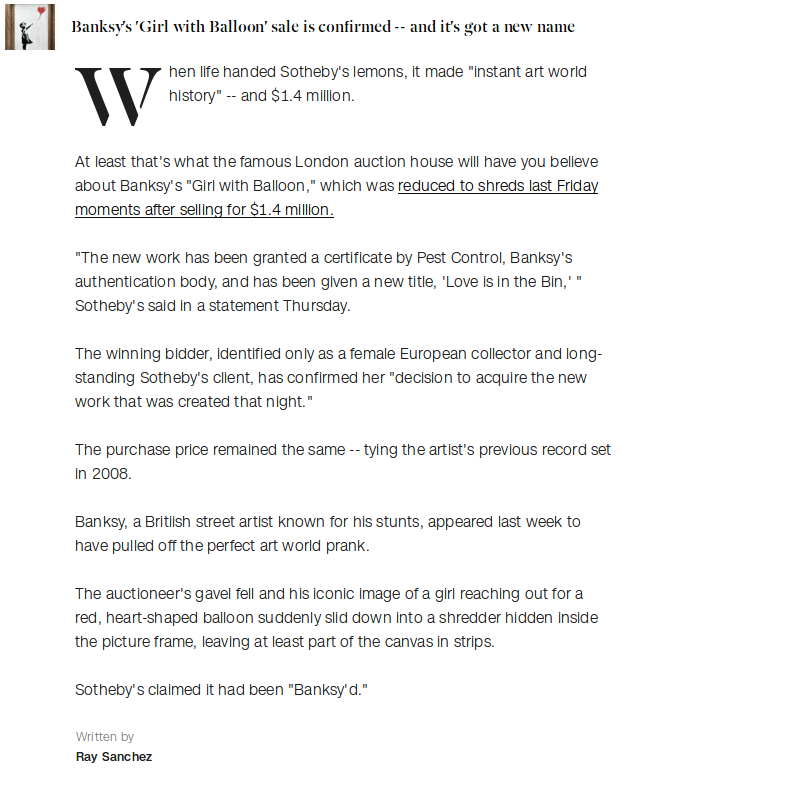
\includegraphics[width=.90\textwidth]{images/ext/article_before.png}};
            \node<3>[inner sep=0pt] (bg) at (0,0)
            {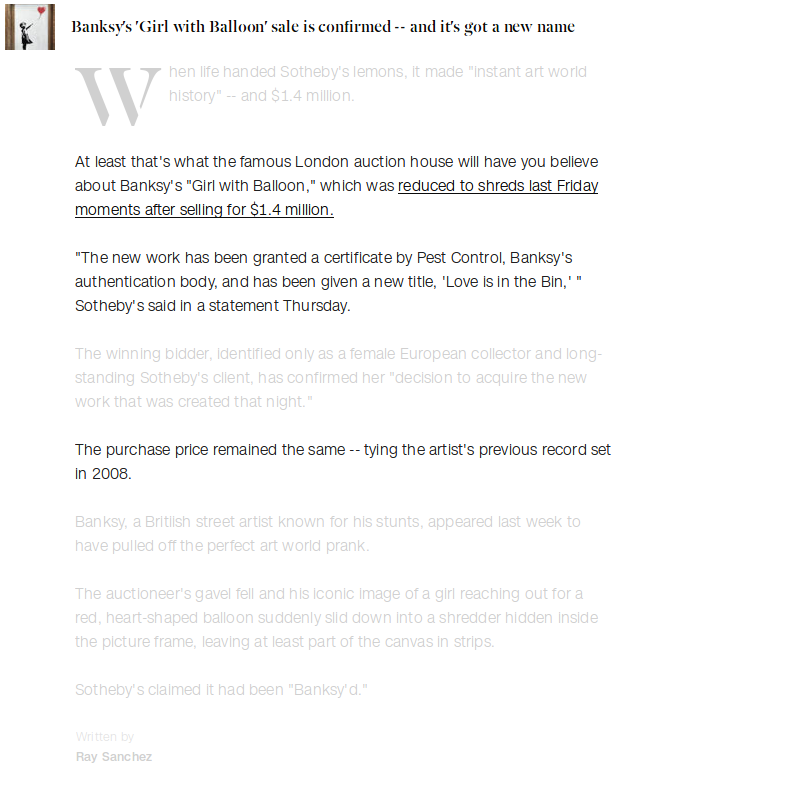
\includegraphics[width=.90\textwidth]{images/ext/article_after.png}};

    \foreach \y/\px [count=\yi] in {0/2.8,1/2.0,1/1.3,0/0.5,1/-0.2,0/-0.8,0/-1.5,0/-2.1}  {
        \node[sent] (s\yi) at (1.5,\px ) {$\uncover<2->{\rightarrow y_\yi}\uncover<3->{=\y}$};
        \node[sent] (s\yi) at (-3.55,\px ) {$s_\yi=$};
    }
    \end{tikzpicture}}
  \end{center}
  \end{column}
  \end{columns}
\end{frame}

\begin{frame}{Deep learning for Extractive Summarization}

  \begin{itemize}
    \item Lots of recent research activity using deep learning for
              summarization!  \\~\\
              
            \begin{center}$\underbrace{p(y_1,\ldots,y_n|s_1,\ldots,s_n;\theta)}_{\text{neural model with parameters $\theta$}}=\prod_{i=1}^n \underbrace{p(y_i|y_{<i},s_1,\ldots,s_n;\theta)}_{\text{salience of $s_i$}}$ \end{center}

              ~\\
              ~\\
    \item Unclear what model design choices are most effective.\\
              \uncover<2>{\alert<2>{We perform a comparison of some task specific
              architectures to simplified or ``standard'' models.\\}}
              ~\\
    \item Unclear what are the most important signals in the data for
              learning.\\
              \uncover<2>{\alert<2>{We perform a several ablation experiments
              to understand the contributions of lexical semantics vs.
              structure/discourse.}}
  \end{itemize}

\end{frame}



\subsection{Model Architectures}

\begin{frame}{Model Architectures}
    \begin{columns}
        \begin{column}{0.4\textwidth}
            Summarization models are hierarchical with the following
            components:
            \begin{itemize}
                \item Word Embedding Layer
                \item Sentence Encoder Layer
                \item Sentence Extractor Layer
            \end{itemize}
        \end{column}
        \begin{column}{0.58\textwidth}
      \resizebox{\textwidth}{!}{
    \begin{tikzpicture}[
            emb/.style={draw,font=\small,outer sep=2pt},
        ]
    \node (s1) at (0,0)  {$s_1=\left[w_1^{(1)},\ldots,w_{l_1}^{(1)}\right]$};
    \node[emb] (embl1) at (0,1.10)  {Word Embedding Layer};
    \draw[->] (s1.north) -- (embl1.south);
    \node (emb1) at (0,2.2) {$\left[\mathbf{w}_1^{(1)},\ldots,\mathbf{w}_{l_1}^{(1)}\right]$};
    \draw[->] (embl1.north) -- (emb1.south);
    \node[emb] (encl1) at (0,3.3)  {Sent. Encoder Layer};
    \draw[->] (emb1.north) -- (encl1.south);
    \node (enc1) at (0,4.3) {$\mathbf{h}_1$};
    \draw[->] (encl1.north) -- (enc1.south);

    \node (s2) at (4,0)  {$s_2=\left[w_1^{(2)},\ldots,w_{l_2}^{(2)}\right]$};
    \node[emb] (embl2) at (4,1.1)  {Word Embedding Layer};
    \draw[->] (s2.north) -- (embl2.south);
    \node (emb2) at (4,2.2) {$\left[\mathbf{w}_1^{(2)},\ldots,\mathbf{w}_{l_2}^{(2)}\right]$};
    \draw[->] (embl2.north) -- (emb2.south);
    \node[emb] (encl2) at (4,3.3)  {Sent. Encoder Layer};
    \draw[->] (emb2.north) -- (encl2.south);
    \node (enc2) at (4,4.3) {$\mathbf{h}_2$};
    \draw[->] (encl2.north) -- (enc2.south);
    
    \node (sn) at (9.0,0)  {$s_n=\left[w_1^{(n)},\ldots,w_{l_n}^{(n)}\right]$};
    \node[emb] (embln) at (9,1.1)  {Word Embedding Layer};
    \draw[->] (sn.north) -- (embln.south);
    \node (embn) at (9,2.2) {$\left[\mathbf{w}_1^{(n)},\ldots,\mathbf{w}_{l_n}^{(n)}\right]$};
    \draw[->] (embln.north) -- (embn.south);
    \node[emb] (encln) at (9,3.3)  {Sent. Encoder Layer};
    \draw[->] (embn.north) -- (encln.south);
    \node (encn) at (9,4.3) {$\mathbf{h}_n$};
    \draw[->] (encln.north) -- (encn.south);
    \draw[->] (encn.north) -- (9,4.9);
    \draw[->] (enc2.north) -- (4,4.9);
    \draw[->] (enc1.north) -- (0,4.9);
    \node[emb,text width=12cm,align=center] at (4.5,5.3) {Sentence Extractor};

    \node at (6.5,0)  {$\large \cdots$};
    \node at (6.5,2.2)  {$\large \cdots$};
    \node at (6.5,4.3)  {$\large \cdots$};

    \node (y1) at (0,6.3) {$y_1$};
    \draw[->] (0,5.7) -- (y1.south);
    \node (y2) at (4,6.3) {$y_2$};
    \draw[->] (4,5.7) -- (y2.south);
    \node (yel) at (6.5,6.3)  {$\cdots$};
    \node (y3) at (9,6.3) {$y_n$};
    \draw[->] (9,5.7) -- (y3.south);
\end{tikzpicture}}
\end{column}
\end{columns}
\end{frame}


\begin{frame}{Sentence Encoders/Extractors}

    \begin{itemize}
        \item We compare 3 different Sentence Encoder Layers:
            \begin{itemize}
                \item Averaging Encoder
                \item CNN Encoder 
                \item RNN Encoder
                \end{itemize}
            \vspace{5pt}
        \item We compare two prior Sentence Extractor Layers,
                SummaRunner Extractor {\tiny (Nallapati et al., 2016)}
                and  Cheng \& Lapata Extractor {\tiny(Cheng and Lapata, 2016)}
                \begin{itemize}
                    \item (SummaRunner only) Internal vector represenatations of summary and document constructed from sentence embeddings.
                    \item Models dependencies between earlier predictions
                        and subsequent predictions.
                \end{itemize}
            \vspace{5pt}
       \item We propose a variant of each Sentence Extractor with less task 
           specific architecture using common neural network components.
            \begin{itemize}
                \item RNN Extractor -- biRNN tagger
                \item Seq2Seq Extractor -- seq2seq with attention
                \begin{itemize}
                    \item No internal represenatations of summary/document.
                    \item Dependencies between predictions not modeled.
            \end{itemize}
            \end{itemize}
    \end{itemize}

\end{frame}



\subsection{Experiments}

\begin{frame}{Experiments}

\begin{itemize}
\item Compare the $3 \times 4$ different encoder/extractor pairings on the single
document sentence extractive summarization task.
\vspace{20pt}

\item Models trained to minimize the negative log-likelihood of training data,
\[\argmin_{\theta} -\sum_{(\mathbf{s}, \mathbf{y}) \in \mathcal{D}} \log p(\mathbf{y}|\mathbf{s};\theta)\]

\item At test time, summaries are generated by sorting sentences in descending order by
    $p(y_i|y_{<i},s_1,\ldots,s_n)$, concatenating, and truncating to $c$ words
\end{itemize}
\end{frame}

\begin{frame}{Datasets}
    \begin{itemize}
        \item News
            \begin{itemize}
                \item CNN/DailyMail (large)
                \item NYT (medium)
                \item DUC (small)
            \end{itemize}
            \vspace{10pt}
        \item Non-News
            \begin{itemize}
                \item Reddit -- Personal Narratives collected by Ouyang and Mckeown (2015) 
                \item AMI  -- Transcripts of office meetings
                \item PubMed -- Medical Journal articles
            \end{itemize}
    \end{itemize}

\end{frame}



\begin{frame}{Experiments \& Ablations}

\begin{itemize} 
    \item Main Experiment
    \begin{itemize}
        \item Embeddings are fixed with GloVe Embeddings 
        \item Learn encoder/extractor parmaters on  Train/Validation splits
    \item Evaluate on Test with \textsc{Rouge}-2 Recall
\end{itemize}
\end{itemize}
\end{frame}

\begin{frame}{Choice of Sentence Encoder: ROUGE-2 Recall}
    \begin{center}

\begin{tabular}{cc ccc ccc} 
        \toprule
        Extractor & Enc.  & CNN/DM & NYT & DUC & Reddit & AMI & PubMed\\
        \midrule
%        Lead &  -- & 24.4 &  32.3 &  21.5 & \textbf{10.9} & 2.0 & 9.3\\
%        \midrule
        \multirow{3}{*}{Seq2Seq} & \alert<2>{Avg.}&\alert<2>{\textbf{25.6}}&\alert<2>{\textbf{35.7}}&\alert<2>{\textbf{22.8}} &
     \alert<2>{\textbf{13.6}} & \alert<2>{\textbf{5.5}} & \alert<2>{\textbf{17.7}}  \\
                         & RNN & 25.3        &\textbf{35.9}& 22.5 &
                     \textbf{12.0} & \textbf{5.3} & 16.7  \\
                         & CNN & 25.1        &  35.1       &\textbf{22.7}&
                     \textbf{13.2} & 2.9 & 16.9  \\
%        \midrule
%\multirow{3}{*}{Cheng \& Lapata} & Avg. & 25.3 & \textbf{35.6} & \textbf{23.1} &
%                        \textbf{13.6} & \textbf{6.1} & \textbf{17.7}  \\
%        
%         & RNN & 25.0 & \textbf{35.8} & \textbf{23.0} &
%                       \textbf{12.6} & \textbf{5.0} & 16.7  \\
%         & CNN & 25.1 & 35.0 & \textbf{23.0} & 
%                       \textbf{13.4} & 2.8 & 16.9  \\
%        \midrule
%        Oracle & -- & 36.2   & 48.9 &  31.8 & 16.2 & 8.7 & 25.0 \\
        \bottomrule
    \end{tabular}
\end{center}

~\\

\begin{itemize}
    \item<2-> \alert<2>{Averaging Sentence Encoder} is either the best encoder or statistically indistinguishable from the best encoder!
    \item<3-> ``Deep'' or compositional understanding of sentences not necessary for good performance.
\end{itemize}


\end{frame}

\begin{frame}{Choice of Sentence Extractor: ROUGE-2 Recall}
        \begin{center}
  \begin{tabular}{cc ccc}
    \toprule
   Extractor & Enc. & CNN/DM & NYT & DUC \\
       % \midrule
       % Random &  --  & 12.7  & 16.0 & 15.8 \\
        \midrule
        Lead &  -- & 24.4  & 32.3  & 21.5 \\
        \midrule
        RNN & Avg. &  25.4  & 34.7  & 22.7 \\
        \alert<2>{ Seq2Seq} & Avg. & \alert<2>{\textbf{25.6}} & \alert<2>{\textbf{35.7}} & \alert<2>{\textbf{22.8}} \\
        \midrule
    Cheng \&  Lapata & Avg. & 25.3 & \textbf{35.6} & \textbf{23.1} \\
    SummaRunner  & Avg. &  25.4 & 35.4 & 22.3 \\
%        \midrule
%        Oracle & -- & 36.2 &  48.9 &  31.8\\
        \bottomrule
    \end{tabular}
\end{center}

\begin{itemize}
    \item   \alert<2>{Seq2Seq Extractor} is the best or statistically indistinguishable from the best system.
    \item<3-> Suggests attention is more important than task specific architecture or representations.
    \end{itemize}

\end{frame}

\begin{frame}{Experiments}
    \begin{itemize}
        \item We find these results suggestive that content is less important to these models.
            \vspace{10pt}
        \item Averaging encoder only gives a shallow representation of sentence meaning.
            \vspace{10pt}
        \item Task specific models that relate sentence representations to 
            documents/summary representations not helpful for performance.

    \end{itemize}
\end{frame}


\begin{frame}{Experiments \& Ablations}
    \begin{itemize}
    \item Embedding Experiment
    \begin{itemize}
        \item Compare performance when embeddings are fine-tuned vs. fixed.
        \item Fine-tuning -- supervised learning of task/domain specific 
            lexical semantics, 
        \item but disrupts the embedding space for words not seen during training, effectively reduces the vocabulary
        
    \end{itemize}
\end{itemize}

\end{frame}

\begin{frame}{Fixed vs. Fine-Tuned Embeddings}
\resizebox{\textwidth}{!}{
\begin{tabular}{cccccccc}
    \toprule
    \multirow{1}{*}{\textbf{Ext.}} &\multirow{1}{*}{\textbf{Emb.}}  & CNN/DM & NYT & DUC & Reddit & \alert<2>{AMI} & PubMed\\
   %  &  & R-2 & R-2 & R-2 & R-2 & R-2 & R-2\\
   % \hline
    \midrule
    \multirow{2}{*}{RNN} & Fixed & \textbf{25.4}\phantom{\scriptsize~(0.2)} & \textbf{34.7}\phantom{\scriptsize~(0.4)} & \textbf{22.7}\phantom{\scriptsize~(0.1)} & \textbf{11.4}\phantom{\scriptsize~(0.1)}& \textbf{ 5.5}\phantom{\scriptsize~(0.2)} & \textbf{17.0}\phantom{\scriptsize~(0.6)}\\
                         & F.-T. & 25.2 \scriptsize{\color{red}(0.2)} & 34.3 \scriptsize{\color{red}(0.4)} & \textbf{22.6} \scriptsize{\color{red}(0.1)} & \textbf{11.3} \scriptsize{\color{red}(0.1)} & \textbf{ 5.3} \scriptsize{\color{red}(0.2)} & 16.4 \scriptsize{\color{red}(0.6)}\\
    \midrule
    \multirow{2}{*}{Seq2Seq} & Fixed & \textbf{25.6}\phantom{\scriptsize~(0.3)}& \textbf{35.7}\phantom{\scriptsize~(0.0)} &  \textbf{22.8}\phantom{\scriptsize~(-0.1)}&  \textbf{13.6}\phantom{\scriptsize~(-0.2)} &  5.5\phantom{\scriptsize~(-0.3)} & \textbf{17.7}\phantom{\scriptsize~(0.8)}\\
   & F.-T. & 25.3 \scriptsize{\color{red}(0.3)} & \textbf{35.7} \scriptsize{\color{red}(0.0)} & \textbf{22.9} \scriptsize{(-0.1)} & \textbf{13.8} \scriptsize{ (-0.2)} & \textbf{ 5.8}  \scriptsize{(-0.3)} & 16.9  \scriptsize{\color{red}(0.8)}\\
 %   \hline
%    \multirow{2}{*}{C\&L} & Fixed & \textbf{25.3} && \textbf{35.6} && \textbf{23.1} && \textbf{13.6} && \textbf{ 6.1} && \textbf{17.7}&\\
%                      & F.-T. & 24.9 &\scriptsize{\color{red}(0.4)} & 35.4 & \scriptsize{\color{red}(0.2)} & \textbf{23.0} &\scriptsize{\color{red} (0.1)} & \textbf{13.4} &\scriptsize{\color{red} (0.2)} & \textbf{ 6.2} &\scriptsize{ (-0.1)} & 16.4 &\scriptsize{\color{red} (1.3)} \\
%    \hline
%\multirow{2}{*}{\begin{tabular}{c} Summa \\ Runner \end{tabular}} & Fixed & \textbf{25.4} && \textbf{35.4} && \textbf{22.3} && \textbf{13.4} && \textbf{ 5.6} & &\textbf{17.2}&\\
%                                                                  & F.-T. & 25.1 &\scriptsize{\color{red}(0.3)} & 35.2 &\scriptsize{\color{red}(0.2)} & \textbf{22.2} & \scriptsize{\color{red}(0.1)} & 12.6 & \scriptsize{\color{red}(0.8)} & \textbf{ 5.8} & \scriptsize{(-0.2)} & 16.8&\scriptsize{\color{red} (0.4) }\\
    \bottomrule
\end{tabular}}

\vspace{10pt}
\begin{itemize}
    \item Only in one case \alert<2>{(AMI)} does fine-tuning embeddings lead to a statistically significant improvement.
\vspace{10pt}
\item<3-> Suggests limited ability or need to learn task-specific 
    lexical-semantics.
    %\item Suggests limited used 
\end{itemize}
\end{frame}




\begin{frame}{Experiments \& Ablations}
\begin{columns}
\begin{column}{0.65\textwidth}
\begin{itemize} 
    \item Part-of-Speech Ablations
    \begin{itemize}
        \item Models are trained on data with different word classes redacted
        \item Redacted words are replaced with a 0 embedding, but position
            of words in sentence is preserved. 
        \item Words are redacted in input, but not when computing \textsc{Rouge}.        
        \item We systematically redact, Nouns, Verbs, Adjectives/Adverbs, Function Words
    \end{itemize}
\end{itemize}
\end{column}

\begin{column}{0.3\textwidth}
\fbox{
\resizebox{0.95\textwidth}{!}{
\begin{minipage}{\textwidth}

%\begin{center}\textbf{Nouns Redacted}\end{center}~\\
%\begin{singlespace}
\tiny
%\begin{enumerate}
 \colorbox{black}{hurricane} \colorbox{black}{gilbert} swept toward the \colorbox{black}{dominican} \colorbox{black}{republic} \colorbox{black}{sunday}, and the \colorbox{black}{civil} \colorbox{black}{defense} alerted its heavily populated south \colorbox{black}{coast} to prepare for high \colorbox{black}{winds}, heavy \colorbox{black}{rains} and high \colorbox{black}{seas}.
 The \colorbox{black}{storm} was approaching from the \colorbox{black}{southeast} with sustained \colorbox{black}{winds} of 75 \colorbox{black}{mph} gusting to 92 \colorbox{black}{mph} .
 ``There is no \colorbox{black}{need} for \colorbox{black}{alarm},'' civil \colorbox{black}{defense} \colorbox{black}{director} \colorbox{black}{eugenio} \colorbox{black}{cabral} said in a \colorbox{black}{television} \colorbox{black}{alert} shortly before \colorbox{black}{midnight} \colorbox{black}{saturday}.
%\item \colorbox{black}{cabral} said \colorbox{black}{residents} of the \colorbox{black}{province} of \colorbox{black}{barahona} should closely follow \colorbox{black}{gilbert}'s \colorbox{black}{movement}.
%\end{enumerate}
%\end{singlespace}
\end{minipage}}}
\end{column}\end{columns}
%?
%?
%?\end{minipage}~~~~~~~\begin{minipage}[t]{0.45\textwidth}
%?\begin{center}\textbf{Verbs Redacted}\end{center}~\\[-50pt]
%?%\begin{singlespace}
%?\small
%?\begin{enumerate}
%?\item Hurricane Gilbert \colorbox{black}{swept} toward the Dominican Republic Sunday, and the Civil Defense \colorbox{black}{alerted} its heavily populated south coast \colorbox{black}{to} \colorbox{black}{prepare} for high winds, heavy rains and high seas.
%?\item The storm \colorbox{black}{was} \colorbox{black}{approaching} from the southeast with sustained winds of 75 mph \colorbox{black}{gusting} to 92 mph.
%?\item ``There \colorbox{black}{is} no need for alarm,'' Civil Defense Director Eugenio Cabral \colorbox{black}{said} in a television alert shortly before midnight Saturday.
%?\item Cabral \colorbox{black}{said} residents of the province of Barahona \colorbox{black}{should} closely \colorbox{black}{follow} Gilbert \colorbox{black}{'s} movement.
%?\end{enumerate}
%?%\end{singlespace}
%?\end{minipage}
%?
%?
%?
%?\end{column}\end{columns}
%?\resizebox{0.1\textwidth}{!}{
%?\fbox{\begin{minipage}{\textwidth}
%?~\\
%?\begin{minipage}[t]{0.45\textwidth}
%?\begin{center}\textbf{Nouns Redacted}\end{center}~\\[-50pt]
%?%\begin{singlespace}
%?\small
%?\begin{enumerate}
%?\item \colorbox{black}{hurricane} \colorbox{black}{gilbert} swept toward the \colorbox{black}{dominican} \colorbox{black}{republic} \colorbox{black}{sunday}, and the \colorbox{black}{civil} \colorbox{black}{defense} alerted its heavily populated south \colorbox{black}{coast} to prepare for high \colorbox{black}{winds}, heavy \colorbox{black}{rains} and high \colorbox{black}{seas}.
%?\item the \colorbox{black}{storm} was approaching from the \colorbox{black}{southeast} with sustained \colorbox{black}{winds} of 75 \colorbox{black}{mph} gusting to 92 \colorbox{black}{mph} .
%?\item ``There is no \colorbox{black}{need} for \colorbox{black}{alarm},'' civil \colorbox{black}{defense} \colorbox{black}{director} \colorbox{black}{eugenio} \colorbox{black}{cabral} said in a \colorbox{black}{television} \colorbox{black}{alert} shortly before \colorbox{black}{midnight} \colorbox{black}{saturday}.
%?\item \colorbox{black}{cabral} said \colorbox{black}{residents} of the \colorbox{black}{province} of \colorbox{black}{barahona} should closely follow \colorbox{black}{gilbert}'s \colorbox{black}{movement}.
%?\end{enumerate}
%?%\end{singlespace}
%?\end{minipage}~~~~~~~\begin{minipage}[t]{0.45\textwidth}
%?\begin{center}\textbf{Verbs Redacted}\end{center}~\\[-50pt]
%?%\begin{singlespace}
%?\small
%?\begin{enumerate}
%?\item Hurricane Gilbert \colorbox{black}{swept} toward the Dominican Republic Sunday, and the Civil Defense \colorbox{black}{alerted} its heavily populated south coast \colorbox{black}{to} \colorbox{black}{prepare} for high winds, heavy rains and high seas.
%?\item The storm \colorbox{black}{was} \colorbox{black}{approaching} from the southeast with sustained winds of 75 mph \colorbox{black}{gusting} to 92 mph.
%?\item ``There \colorbox{black}{is} no need for alarm,'' Civil Defense Director Eugenio Cabral \colorbox{black}{said} in a television alert shortly before midnight Saturday.
%?\item Cabral \colorbox{black}{said} residents of the province of Barahona \colorbox{black}{should} closely \colorbox{black}{follow} Gilbert \colorbox{black}{'s} movement.
%?\end{enumerate}
%?%\end{singlespace}
%?\end{minipage}
%?
%?~\\
%?~\\
%?
%?\begin{minipage}{0.45\textwidth}
%?\begin{center}\textbf{Adjectives/Adverbs Redacted}\end{center}~\\[-50pt]
%?%\begin{singlespace}
%?\small
%?\begin{enumerate}
%?\item Hurricane Gilbert swept toward the Dominican Republic Sunday, and the Civil Defense alerted \colorbox{black}{its} \colorbox{black}{heavily} \colorbox{black}{populated} \colorbox{black}{south} coast to prepare for \colorbox{black}{high} winds, \colorbox{black}{heavy} rains and \colorbox{black}{high} seas.
%?\item The storm was approaching from the southeast with \colorbox{black}{sustained} winds of 75 mph gusting to 92 mph.
%?\item ``\colorbox{black}{there} is no need for alarm,'' \colorbox{black}{civil} Defense Director Eugenio Cabral said in a television alert \colorbox{black}{shortly} before midnight Saturday.
%?\item Cabral said residents of the province of Barahona should \colorbox{black}{closely} follow Gilbert's movement.
%?\end{enumerate}
%?%\end{singlespace}
%?\end{minipage}~~~~~~~\begin{minipage}{0.45\textwidth}
%?\begin{center}\textbf{Function Words Redacted}\end{center}~\\[-50pt]
%?%\begin{singlespace}
%?\small
%?\begin{enumerate}
%?\item Hurricane Gilbert swept \colorbox{black}{toward} \colorbox{black}{the} Dominican Republic Sunday, \colorbox{black}{and} \colorbox{black}{the} Civil Defense alerted its heavily populated south coast to prepare \colorbox{black}{for} high winds, heavy rains \colorbox{black}{and} high seas.
%?\item \colorbox{black}{the} storm was approaching \colorbox{black}{from} \colorbox{black}{the} southeast \colorbox{black}{with} sustained winds \colorbox{black}{of} 75 mph gusting \colorbox{black}{to} 92 mph .
%?\item ``There is \colorbox{black}{no} need \colorbox{black}{for} alarm,'' Civil Defense Director Eugenio Cabral said \colorbox{black}{in} \colorbox{black}{a} television alert shortly \colorbox{black}{before} midnight Saturday.
%?\item Cabral said residents \colorbox{black}{of} \colorbox{black}{the} province \colorbox{black}{of} Barahona should closely follow Gilbert's movement.
%?\end{enumerate}
%?%\end{singlespace}
%?\end{minipage}
%?
%?~\\
%?\end{minipage}}
%?}
%?\end{column}
%?\end{columns}

\end{frame}

\begin{frame}{Part-of-Speech Ablation}
\begin{center}
\begin{tabular}{ccccccc}
    \toprule
    \multirow{1}{*}{\textbf{Ablation}}  & \multicolumn{1}{c}{\textbf{CNN/DM}} & \multicolumn{1}{c}{\textbf{NYT}} & \multicolumn{1}{c}{\textbf{DUC}} & \multicolumn{1}{c}{\textbf{Reddit}} & \multicolumn{1}{c}{\textbf{AMI}} & \multicolumn{1}{c}{\textbf{PubMed}}\\
    \hline
    all words & \textbf{25.4} & \textbf{34.7} & 22.7 & \textbf{11.4} & 5.5 & \textbf{17.0}  \\
    \alert<5>{ -nouns}    & 25.3 & 34.3 & 22.3 & 10.3 & \alert<5>{3.8} & \alert<5>{15.7} \\
    -verbs    & 25.3 & 34.4 & 22.4 & 10.8 & 5.8 & 16.6 \\
    \alert<4>{-adj/adv}  & 25.3 & 34.4 & 22.5          & \alert<4>{9.5}  & 5.4 & 16.8 \\
    -function & 25.2 & 34.5 & \textbf{22.9} & 10.3 & \textbf{6.3} & 16.6 \\
\midrule
Max Diff. & \alert<2>{0.2} & \alert<2>{0.4} & \alert<2>{0.4} & \alert<3>{1.9} & \alert<3>{1.7} & \alert<3>{1.3} \\ 
    \bottomrule
\end{tabular}
\end{center}

\begin{itemize}
\item<2-> News is relatively robust to word class ablations.
\item<3-> Non-news domains more sensitive to content based features. 
\item<4-> \alert<4>{Adjectives/Adverbs} especially important to personal narratives.
\item<5-> \alert<5>{Nouns} especially important to meetings/research.

\end{itemize}

\end{frame}




\begin{frame}{Experiments \& Ablations}
\begin{columns}
    \begin{column}{0.5\textwidth}
\begin{itemize}
    \item Document Shuffling
        \begin{itemize}
            \item Sentence order is shuffled during training, so
                \vspace{5pt}
            \item position is obscured as a heuristic that can be exploited,
                \vspace{5pt}
             \item model must rely on content-derived features.
                \vspace{5pt}
             \item At test time, document is presented in original order.
        \end{itemize}
\end{itemize}
\end{column}
\begin{column}{0.5\textwidth}
    \[ p(\mathbf{y}|s_1, s_2, s_3, s_4) \rightarrow p(\mathbf{y}|s_2, s_4, s_1,s_3)   \]
\end{column}
\end{columns}
\end{frame}

\begin{frame}{Document Shuffling}

\resizebox{\textwidth}{!}{
\begin{tabular}{cccccccc}
    \toprule
    \textbf{Ext.} &\textbf{Order}  & CNN/DM & NYT & DUC & Reddit & AMI & PubMed\\
    \midrule
    \multirow{2}{*}{Seq2Seq} & In-Order & \textbf{25.6} &  \textbf{35.7}  & \textbf{22.8} &  \textbf{13.6}& 5.5 & \textbf{17.7} \\
                             & Shuffled & 21.7  & 25.6   & 21.2  &\textbf{13.5}  &\alert<4>{\textbf{6.0}} &14.9 \\
\midrule
& Diff. & \alert<2>{3.9} & \alert<2>{10.1} & \alert<2>{1.6} & 0.1 & -0.5 & \alert<2>{2.8} \\
    \bottomrule
\end{tabular}}

\begin{itemize}
    \item<2-> News and Research paper domain models are more sensitive to
position.
\item <3->Suggests news/research models are mostly exploiting position and not content
\item<4-> \alert<4>{AMI actually improves,} suggesting removing position features from
    domains where this heurisitic is not reliable is helpful.
\end{itemize}

\end{frame}

\begin{frame}{Takeaways}


    \begin{itemize}
        \item Our main contribution in this section is a thorough evaluation of neural sentence extraction
models for single document summarization.
\vspace{10pt}
        \item Our findings reveal that
            in the presence of shallow heuristics, content/semantics of sentences
        less important to models.
        \begin{itemize}
            \item Averaging encoder works better than order-aware models.
            \item Explicitly modeling summaries/documents/output dependencies not necessary to achieve best performance.
            \item Task-specific word embeddings little to no improvement over
                 generic embeddings.
            \item News models where position is exploitable show small drops in performance  under word-class ablations.
            \item Removing position as a feature drops performance significantly on news.
         \end{itemize}
         \vspace{10pt}

    \end{itemize}
 \end{frame}

 \begin{frame}{Takeaways}

     \begin{itemize}

        \item This is important to know because we should not expect neural summarization models
            trained on large news datasets  to 
            perform well where content is important for predicting sentence salience.
         \vspace{10pt}

     \item Our findings also suggest that abstractive summarization models will not be effective on tasks
         that require complex reasoning about the content.
         \vspace{10pt}
     \item Summarization research should focus on problems other
         than single document news summarization for estimating salience
         since position is so strong a feature.

         \vspace{10pt}

     \item  To that end, we turn to stream summarization, where position
         is a less reliable heuristic.


 \end{itemize}
 \end{frame}

%\begin{frame}{Takeaways}
%                \begin{itemize}
%                    \item How to represent sentences? \alert{Averaging is effective!}
%
%                    \item How to model salience of sentences w.r.t. document context? \alert{Seq2seq + attention mechanism as good as task specific architectures.}
%                    \item Simpler or More generic architecture choices as good as task specific ones. \alert{Explicitly representing documents/summaries/dependencies amongst output variables less important.}
%\item \alert{Heuristics exploitable by the models have more of an impact than modeling choices in this task.}
%                \end{itemize}
%
%
%\end{frame}


\section{Salience Estimation with Structured Content Selection Models}
  
\subsection{Task}

\begin{frame}[fragile]{Query Focused, Sentence Extractive, Stream Summarization}
\resizebox{0.99\textwidth}{!}{
  \begin{tikzpicture}
    \tikzstyle{sent}=[align=left]
    %\draw (0,8) rectangle (10,0);
    \draw[red] (0,8.5) rectangle (18,0);
 
    \node at (7.45,8.1) [draw,rounded corners,very thick] 
    {\tiny ~ 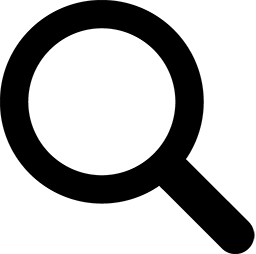
\includegraphics[scale=.02]{images/strm/magnify} 
     ~ ``Hurricane Sandy''};
    %\draw[orange!20,fill=orange!20] (0,7.5) rectangle (1.7,4);
    %\draw[orange!20,fill=orange!20] (0,3.95) rectangle (1.7,.45);
 
    \draw[white,top color=orange,bottom color=orange!20,shading=axis,
          shading angle=16] (0,2) -- (0,0) -- (1.7,0) -- 
            (1.7,2) -- (0,2) -- cycle; 
    \draw[white,top color=orange,bottom color=orange!20,shading=axis,
          shading angle=165] (0,5) -- (0,2) -- (.85,1) -- (1.7,2) -- 
            (1.7,5) -- (0,5) -- cycle; 

    \draw[white,top color=orange,bottom color=orange!20,shading=axis,
          shading angle=25] (0,8) -- (0,5) -- (0.85,4) -- (1.7,5) -- 
            (1.7,8) -- (0,8) -- cycle;
    \draw[white,top color=orange!90,bottom color=orange!20,shading=axis,
          shading angle=25] (0,8) -- (0.85,7) -- (1.7,8) -- (0,8) -- cycle;

    \node[rotate=90,text=white] at (.85,5.8) {\Huge 2:00};
    \node[rotate=90,text=white] at (.85,2.8) {\Huge 3:00};

  \node (f) at (2,6.55) {
  \begin{tikzpicture}[transform canvas={scale=0.2}]
    \tikzstyle{sent}=[align=left]
    \tikzstyle{doc}=[rectangle,rounded corners,draw=black, very thick]

    \draw (-.02,4.75) node  [
    very thick,
    weird fill=blue!10,
    text width=0.15cm,align=center,text height=1.8cm] {};
    \draw[doc] (-.25,5.80) rectangle (9.5, 3.70); 
    \node[sent,left] at (9.5, 5.5) {\fontsize{7}{11}\selectfont ... two bombs went off at the 
        finish line of the Boston  Marathon.};
    \node[sent,left] at (9.5, 5) {\fontsize{7}{11}\selectfont Many of the injured were 
        reportedly bystanders.};
    \node[sent,left] at (9.5, 4.5) {\fontsize{7}{11}\selectfont The blasts reportedly happened 
        across the street from the Lenox Hotel.};
    \node[sent,left] at (9.5, 4) {\fontsize{7}{11}\selectfont We will update you on any 
        breaking news we hear about this.};
    \node[rotate=90] at (0,4.75) {\tiny 3:05 pm} ;

    \draw (-.02,2.5) node  [
    very thick,
    weird fill=blue!10,
    text width=0.15cm,align=center,text height=1.3cm] {};
    \draw[doc] (-.25,3.30) rectangle (9.5, 1.70); 
    \node[sent,left] at (9.5, 3) {\fontsize{7}{11}\selectfont ... two bombs were detonated at 
        the race's finish line, killing and injuring many.};
    \node[sent,left] at (9.5, 2.5) {\fontsize{7}{11}\selectfont ... two more explosive devices
         have been found.};
    \node[sent,left] at (9.5, 2.0) {\fontsize{7}{11}\selectfont The White House says President 
        Obama has been notified about the explosions.};
    \node[rotate=90] at (0,2.5) {\tiny 3:45 pm} ;

    \draw (-.02,0.75) node  [
    very thick,
    weird fill=blue!10,
    text width=0.15cm,align=center,text height=0.8cm] {};
    \node[rotate=90] at (0,0.75) {\tiny 3:55 pm} ;
    \draw[doc] (-.25,1.30) rectangle (9.5,.2); 
    \node[sent,left] at (9.5, 1.0) {\fontsize{7}{11}\selectfont NBC news reports that 
        ``multiple explosive devices'' have been found in Boston.};
    \node[sent,left] at (9.5, 0.5) {\fontsize{7}{11}\selectfont Boston police report
        that two people were killed and at least 22 injured.};


  \end{tikzpicture}
  };
 \node (c) at (2,5.05) {
  \begin{tikzpicture}[transform canvas={scale=0.2}]
    \tikzstyle{sent}=[align=left]
    \tikzstyle{doc}=[rectangle,rounded corners,draw=black, very thick]


    \draw (-.02,6.75) node  [
    very thick,
    weird fill=blue!10,
    text width=0.15cm,align=center,text height=0.8cm] {};
    \draw[doc] (-.25,7.30) rectangle (9.5, 6.20); 
    \node[sent,left] at (9.5, 7) {\fontsize{7}{11}\selectfont Moments ago there were 
        explosions near the finish line of the Boston Marathon.}; 
    \node[sent,left] at (9.5, 6.5) {\fontsize{7}{11}\selectfont It has not been confirmed, 
        but its quite likely these were bombings.};
    \node[rotate=90] at (0,6.75) {\tiny 3:00 pm} ;
    
    \draw (-.02,4.75) node  [
    very thick,
    weird fill=blue!10,
    text width=0.15cm,align=center,text height=1.8cm] {};
    \draw[doc] (-.25,5.80) rectangle (9.5, 3.70); 
    \node[sent,left] at (9.5, 5.5) {\fontsize{7}{11}\selectfont ... two bombs went off at the 
        finish line of the Boston  Marathon.};
    \node[sent,left] at (9.5, 5) {\fontsize{7}{11}\selectfont Many of the injured were 
        reportedly bystanders.};
    \node[sent,left] at (9.5, 4.5) {\fontsize{7}{11}\selectfont The blasts reportedly happened 
        across the street from the Lenox Hotel.};
    \node[sent,left] at (9.5, 4) {\fontsize{7}{11}\selectfont We will update you on any 
        breaking news we hear about this.};
    \node[rotate=90] at (0,4.75) {\tiny 3:05 pm} ;

    \draw (-.02,2.5) node  [
    very thick,
    weird fill=blue!10,
    text width=0.15cm,align=center,text height=1.3cm] {};
    \draw[doc] (-.25,3.30) rectangle (9.5, 1.70); 
    \node[sent,left] at (9.5, 3) {\fontsize{7}{11}\selectfont ... two bombs were detonated at 
        the race's finish line, killing and injuring many.};
    \node[sent,left] at (9.5, 2.5) {\fontsize{7}{11}\selectfont ... two more explosive devices
         have been found.};
    \node[sent,left] at (9.5, 2.0) {\fontsize{7}{11}\selectfont The White House says President 
        Obama has been notified about the explosions.};
    \node[rotate=90] at (0,2.5) {\tiny 3:45 pm} ;

    \draw (-.02,0.75) node  [
    very thick,
    weird fill=blue!10,
    text width=0.15cm,align=center,text height=0.8cm] {};
    \node[rotate=90] at (0,0.75) {\tiny 3:55 pm} ;
    \draw[doc] (-.25,1.30) rectangle (9.5,.2); 
    \node[sent,left] at (9.5, 1.0) {\fontsize{7}{11}\selectfont NBC news reports that 
        ``multiple explosive devices'' have been found in Boston.};
    \node[sent,left] at (9.5, 0.5) {\fontsize{7}{11}\selectfont Boston police report
        that two people were killed and at least 22 injured.};


  \end{tikzpicture}
  };

  \node (a) at (2,3.5) {
  \begin{tikzpicture}[transform canvas={scale=0.2}]
    \tikzstyle{sent}=[align=left]
    \tikzstyle{doc}=[rectangle,rounded corners,draw=black, very thick]

    \draw[black,rounded corners,very thick,dotted] (-0.5,7.5) rectangle (9.75,0);

    \draw (-.02,6.75) node  [
    very thick,
    weird fill=blue!10,
    text width=0.15cm,align=center,text height=0.8cm] {};
    \draw[doc] (-.25,7.30) rectangle (9.5, 6.20); 
    \node[sent,left] at (9.5, 7) {\fontsize{7}{11}\selectfont Moments ago there were 
        explosions near the finish line of the Boston Marathon.}; 
    \node[sent,left] at (9.5, 6.5) {\fontsize{7}{11}\selectfont It has not been confirmed, 
        but its quite likely these were bombings.};
    \node[rotate=90] at (0,6.75) {\tiny 3:00 pm} ;
    
    \draw (-.02,4.75) node  [
    very thick,
    weird fill=blue!10,
    text width=0.15cm,align=center,text height=1.8cm] {};
    \draw[doc] (-.25,5.80) rectangle (9.5, 3.70); 
    \node[sent,left] at (9.5, 5.5) {\fontsize{7}{11}\selectfont ... two bombs went off at the 
        finish line of the Boston  Marathon.};
    \node[sent,left] at (9.5, 5) {\fontsize{7}{11}\selectfont Many of the injured were 
        reportedly bystanders.};
    \node[sent,left] at (9.5, 4.5) {\fontsize{7}{11}\selectfont The blasts reportedly happened 
        across the street from the Lenox Hotel.};
    \node[sent,left] at (9.5, 4) {\fontsize{7}{11}\selectfont We will update you on any 
        breaking news we hear about this.};
    \node[rotate=90] at (0,4.75) {\tiny 3:05 pm} ;

    \draw (-.02,2.5) node  [
    very thick,
    weird fill=blue!10,
    text width=0.15cm,align=center,text height=1.3cm] {};
    \draw[doc] (-.25,3.30) rectangle (9.5, 1.70); 
    \node[sent,left] at (9.5, 3) {\fontsize{7}{11}\selectfont ... two bombs were detonated at 
        the race's finish line, killing and injuring many.};
    \node[sent,left] at (9.5, 2.5) {\fontsize{7}{11}\selectfont ... two more explosive devices
         have been found.};
    \node[sent,left] at (9.5, 2.0) {\fontsize{7}{11}\selectfont The White House says President 
        Obama has been notified about the explosions.};
    \node[rotate=90] at (0,2.5) {\tiny 3:45 pm} ;

    \draw (-.02,0.75) node  [
    very thick,
    weird fill=blue!10,
    text width=0.15cm,align=center,text height=0.8cm] {};
    \node[rotate=90] at (0,0.75) {\tiny 3:55 pm} ;
    \draw[doc] (-.25,1.30) rectangle (9.5,.2); 
    \node[sent,left] at (9.5, 1.0) {\fontsize{7}{11}\selectfont NBC news reports that 
        ``multiple explosive devices'' have been found in Boston.};
    \node[sent,left] at (9.5, 0.5) {\fontsize{7}{11}\selectfont Boston police report
        that two people were killed and at least 22 injured.};


  \end{tikzpicture}
  };

 \node (d) at (2,2.00) {
  \begin{tikzpicture}[transform canvas={scale=0.2}]
    \tikzstyle{sent}=[align=left]
    \tikzstyle{doc}=[rectangle,rounded corners,draw=black, very thick]


    \draw (-.02,6.75) node  [
    very thick,
    weird fill=blue!10,
    text width=0.15cm,align=center,text height=0.8cm] {};
    \draw[doc] (-.25,7.30) rectangle (9.5, 6.20); 
    \node[sent,left] at (9.5, 7) {\fontsize{7}{11}\selectfont Moments ago there were 
        explosions near the finish line of the Boston Marathon.}; 
    \node[sent,left] at (9.5, 6.5) {\fontsize{7}{11}\selectfont It has not been confirmed, 
        but its quite likely these were bombings.};
    \node[rotate=90] at (0,6.75) {\tiny 3:00 pm} ;
    
    \draw (-.02,4.75) node  [
    very thick,
    weird fill=blue!10,
    text width=0.15cm,align=center,text height=1.8cm] {};
    \draw[doc] (-.25,5.80) rectangle (9.5, 3.70); 
    \node[sent,left] at (9.5, 5.5) {\fontsize{7}{11}\selectfont ... two bombs went off at the 
        finish line of the Boston  Marathon.};
    \node[sent,left] at (9.5, 5) {\fontsize{7}{11}\selectfont Many of the injured were 
        reportedly bystanders.};
    \node[sent,left] at (9.5, 4.5) {\fontsize{7}{11}\selectfont The blasts reportedly happened 
        across the street from the Lenox Hotel.};
    \node[sent,left] at (9.5, 4) {\fontsize{7}{11}\selectfont We will update you on any 
        breaking news we hear about this.};
    \node[rotate=90] at (0,4.75) {\tiny 3:05 pm} ;

    \draw (-.02,2.5) node  [
    very thick,
    weird fill=blue!10,
    text width=0.15cm,align=center,text height=1.3cm] {};
    \draw[doc] (-.25,3.30) rectangle (9.5, 1.70); 
    \node[sent,left] at (9.5, 3) {\fontsize{7}{11}\selectfont ... two bombs were detonated at 
        the race's finish line, killing and injuring many.};
    \node[sent,left] at (9.5, 2.5) {\fontsize{7}{11}\selectfont ... two more explosive devices
         have been found.};
    \node[sent,left] at (9.5, 2.0) {\fontsize{7}{11}\selectfont The White House says President 
        Obama has been notified about the explosions.};
    \node[rotate=90] at (0,2.5) {\tiny 3:45 pm} ;

    \draw (-.02,0.75) node  [
    very thick,
    weird fill=blue!10,
    text width=0.15cm,align=center,text height=0.8cm] {};
    \node[rotate=90] at (0,0.75) {\tiny 3:55 pm} ;
    \draw[doc] (-.25,1.30) rectangle (9.5,.2); 
    \node[sent,left] at (9.5, 1.0) {\fontsize{7}{11}\selectfont NBC news reports that 
        ``multiple explosive devices'' have been found in Boston.};
    \node[sent,left] at (9.5, 0.5) {\fontsize{7}{11}\selectfont Boston police report
        that two people were killed and at least 22 injured.};


  \end{tikzpicture}
  };




\node (e) at (2,0.2) {
  \begin{tikzpicture}[transform canvas={scale=0.2}]
    \tikzstyle{sent}=[align=left]
    \tikzstyle{doc}=[rectangle,rounded corners,draw=black, very thick]

    \draw (-.02,8.25) node  [
    very thick,
    weird fill=blue!10,
    text width=0.15cm,align=center,text height=0.8cm] {};
    \draw[doc] (-.25,8.8) rectangle (9.5, 7.70); 
    \node[sent,left] at (9.5, 8.5) {\fontsize{7}{11}\selectfont Moments ago there were 
        explosions near the finish line of the Boston Marathon.}; 
    \node[sent,left] at (9.5, 8) {\fontsize{7}{11}\selectfont It has not been confirmed, 
        but its quite likely these were bombings.};
    \node[rotate=90] at (0,8.25) {\tiny 3:00 pm} ;
 
    \draw (-.02,6.75) node  [
    very thick,
    weird fill=blue!10,
    text width=0.15cm,align=center,text height=0.8cm] {};
    \draw[doc] (-.25,7.30) rectangle (9.5, 6.20); 
    \node[sent,left] at (9.5, 7) {\fontsize{7}{11}\selectfont Moments ago there were 
        explosions near the finish line of the Boston Marathon.}; 
    \node[sent,left] at (9.5, 6.5) {\fontsize{7}{11}\selectfont It has not been confirmed, 
        but its quite likely these were bombings.};
    \node[rotate=90] at (0,6.75) {\tiny 3:00 pm} ;
    
    \draw (-.02,4.75) node  [
    very thick,
    weird fill=blue!10,
    text width=0.15cm,align=center,text height=1.8cm] {};
    \draw[doc] (-.25,5.80) rectangle (9.5, 3.70); 
    \node[sent,left] at (9.5, 5.5) {\fontsize{7}{11}\selectfont ... two bombs went off at the 
        finish line of the Boston  Marathon.};
    \node[sent,left] at (9.5, 5) {\fontsize{7}{11}\selectfont Many of the injured were 
        reportedly bystanders.};
    \node[sent,left] at (9.5, 4.5) {\fontsize{7}{11}\selectfont The blasts reportedly happened 
        across the street from the Lenox Hotel.};
    \node[sent,left] at (9.5, 4) {\fontsize{7}{11}\selectfont We will update you on any 
        breaking news we hear about this.};
    \node[rotate=90] at (0,4.75) {\tiny 3:05 pm} ;

    \draw (-.02,2.5) node  [
    very thick,
    weird fill=blue!10,
    text width=0.15cm,align=center,text height=1.3cm] {};
    \draw[doc] (-.25,3.30) rectangle (9.5, 1.70); 
    \node[sent,left] at (9.5, 3) {\fontsize{7}{11}\selectfont ... two bombs were detonated at 
        the race's finish line, killing and injuring many.};
    \node[sent,left] at (9.5, 2.5) {\fontsize{7}{11}\selectfont ... two more explosive devices
         have been found.};
    \node[sent,left] at (9.5, 2.0) {\fontsize{7}{11}\selectfont The White House says President 
        Obama has been notified about the explosions.};
    \node[rotate=90] at (0,2.5) {\tiny 3:45 pm} ;

    \draw (-.02,0.75) node  [
    very thick,
    weird fill=blue!10,
    text width=0.15cm,align=center,text height=0.8cm] {};
    \node[rotate=90] at (0,0.75) {\tiny 3:55 pm} ;
    \draw[doc] (-.25,1.30) rectangle (9.5,.2); 
    \node[sent,left] at (9.5, 1.0) {\fontsize{7}{11}\selectfont NBC news reports that 
        ``multiple explosive devices'' have been found in Boston.};
    \node[sent,left] at (9.5, 0.5) {\fontsize{7}{11}\selectfont Boston police report
        that two people were killed and at least 22 injured.};


  \end{tikzpicture}
  };






\only<1>{
    \draw[dashed] (1.90,5) -- (4.8,7.5);
    \draw[dashed] (3.95,5) -- (8.9,7.5);
    \draw[dashed] (1.90,3.5) -- (4.8,4.5);
    \draw[dashed] (3.95,3.5) -- (8.9,4.5);

   \node (b) at (5,4.5) {
  \begin{tikzpicture}[transform canvas={scale=0.4}]
    \tikzstyle{sent}=[align=left]
    \tikzstyle{doc}=[rectangle,rounded corners,draw=black, very thick]

    \draw[black,rounded corners,very thick,fill=white] (-0.5,7.5) rectangle (9.75,0);

    \draw (-.02,6.75) node  [
    very thick,
    weird fill=blue!10,
    text width=0.15cm,align=center,text height=0.8cm] {};
    \draw[doc] (-.25,7.30) rectangle (9.5, 6.20); 
    \node[sent,left] at (9.5, 7) {\fontsize{7}{11}\selectfont Moments ago there were 
        explosions near the finish line of the Boston Marathon.}; 
    \node[sent,left] at (9.5, 6.5) {\fontsize{7}{11}\selectfont It has not been confirmed, 
        but its quite likely these were bombings.};
    \node[rotate=90] at (0,6.75) {\tiny 3:00 pm} ;
    
    \draw (-.02,4.75) node  [
    very thick,
    weird fill=blue!10,
    text width=0.15cm,align=center,text height=1.8cm] {};
    \draw[doc] (-.25,5.80) rectangle (9.5, 3.70); 
    \node[sent,left] at (9.5, 5.5) {\fontsize{7}{11}\selectfont ... two bombs went off at the 
        finish line of the Boston  Marathon.};
    \node[sent,left] at (9.5, 5) {\fontsize{7}{11}\selectfont Many of the injured were 
        reportedly bystanders.};
    \node[sent,left] at (9.5, 4.5) {\fontsize{7}{11}\selectfont The blasts reportedly happened 
        across the street from the Lenox Hotel.};
    \node[sent,left] at (9.5, 4) {\fontsize{7}{11}\selectfont We will update you on any 
        breaking news we hear about this.};
    \node[rotate=90] at (0,4.75) {\tiny 3:05 pm} ;

    \draw (-.02,2.5) node  [
    very thick,
    weird fill=blue!10,
    text width=0.15cm,align=center,text height=1.3cm] {};
    \draw[doc] (-.25,3.30) rectangle (9.5, 1.70); 
    \node[sent,left] at (9.5, 3) {\fontsize{7}{11}\selectfont ... two bombs were detonated at 
        the race's finish line, killing and injuring many.};
    \node[sent,left] at (9.5, 2.5) {\fontsize{7}{11}\selectfont ... two more explosive devices
         have been found.};
    \node[sent,left] at (9.5, 2.0) {\fontsize{7}{11}\selectfont The White House says President 
        Obama has been notified about the explosions.};
    \node[rotate=90] at (0,2.5) {\tiny 3:45 pm} ;

    \draw (-.02,0.75) node  [
    very thick,
    weird fill=blue!10,
    text width=0.15cm,align=center,text height=0.8cm] {};
    \node[rotate=90] at (0,0.75) {\tiny 3:55 pm} ;
    \draw[doc] (-.25,1.30) rectangle (9.5,.2); 
    \node[sent,left] at (9.5, 1.0) {\fontsize{7}{11}\selectfont NBC news reports that 
        ``multiple explosive devices'' have been found in Boston.};
    \node[sent,left] at (9.5, 0.5) {\fontsize{7}{11}\selectfont Boston police report
        that two people were killed and at least 22 injured.};


  \end{tikzpicture}
  };
}


\uncover<2>{
\node[anchor=north west,text width=12cm] at (5,7) {
\begin{itemize}
\item Summarization system must monitor a continuously updating stream of news documents, and extract updates related to the query.
    \vspace{10pt}
\item Update Summary --- a continuously updated collection of extracted 
    sentences that summarize the event.
    \vspace{10pt}

\item Updates --- an extracted sentence from the stream; updates should contain
    novel and timely informtation.
    \vspace{10pt}

\item Salience --- decreases over time
\end{itemize}
};
}

\uncover<3,4>{
\node[anchor=north west,text width=12cm] at (5,8) {
    \begin{itemize}
        \item Nuggets --- atomic facts, essential to the query
        \vspace{5pt}
        \begin{itemize}
            \item A good update summary contains mostly ``nugget'' information
            \vspace{5pt}
            \item Nuggets are manually extracted from Wikipedia
        \end{itemize}
        \vspace{10pt}
        \item Example Nuggets for query "Hurricane Sandy"
        \vspace{5pt}
        %\begin{itemize}
            \colorbox{red!20}{\small [A] At least 80 homes were completely destroyed by fire in the Breezy Point, Queens} \\
            \colorbox{green!20}{\small [B] Seven subway tunnels under the East River flooded} \\
            \colorbox{blue!20}{\small [C] Sandy left power outages} \\
       % \vspace{5pt}
       %     \item Example A
       % \vspace{5pt}
       %     \item Example A
        %\end{itemize}

        \vspace{10pt}
        \item Extracted updates should ``contain'' novel nuggets \\
      \textit{\small New York City officials spent the day grappling with the damage from Sandy, the Atlantic superstorm that killed 10 people, \colorbox{red!20}{sparked a fire that destroyed 111 homes in Queens,} \colorbox{green!20}{flooded tunnels of the biggest U.S. transit system} and \colorbox{blue!20}{left more than 750,000 customers without power.}}


    \end{itemize}
};
            }
            \uncover<4->{
            \node[inner sep=1pt,fill=yellow,text=red,draw=red,font=\tiny] at (4.1,7.1) {A};
            \node[inner sep=1pt,fill=yellow,text=red,draw=red,font=\tiny] at (4.5,7.1) {B};
            \node[inner sep=1pt,fill=yellow,text=red,draw=red,font=\tiny] at (4.1,6.7) {C};

            \node[inner sep=1pt,fill=yellow,text=red,draw=red,font=\tiny] at (4.1,6.1) {A};
            \node[inner sep=1pt,fill=yellow,text=red,draw=red,font=\tiny] at (4.1,5.7) {B};
            \node[inner sep=1pt,fill=yellow,text=red,draw=red,font=\tiny] at (4.1,4.1) {A};
            \node[inner sep=1pt,fill=yellow,text=red,draw=red,font=\tiny] at (4.5,4.1) {C};
            \node[inner sep=1pt,fill=yellow,text=red,draw=red,font=\tiny] at (4.1,3.1) {B};
            \node[inner sep=1pt,fill=yellow,text=red,draw=red,font=\tiny] at (4.1,2.1) {A};
            \node[inner sep=1pt,fill=yellow,text=red,draw=red,font=\tiny] at (4.1,0.5) {A};
            }


            \uncover<5-12>{
\node[anchor=north west,text width=12cm] at (5,7) {
    \begin{itemize}
        \item System Time --- the position in the news stream.
                    \vspace{5pt}
            \begin{itemize}
                \item The summarization system  can extract any sentence from the stream earlier than the system time.
                    \vspace{5pt}
                \item System time can be incremented in arbitrary positive amounts.
%                
            \end{itemize}
    \end{itemize}
};
}

\uncover<6>{

    \draw[opacity=0.75,fill=white,draw=white]  ($(c.south east)+(2.75,0.1)$) rectangle ($(c.south east)+(-0.3,-4.9)$);
    \node (T1) at ($(c.south east)+(3,0)$) {$\quad\tau_i$};
    \draw[-,line width=0.5mm] ($(c.south east)+(2.75,0.1)$) -- ($(c.south east)+(-0.2,0.1)$);


}
\uncover<7>{

    \draw[opacity=0.75,fill=white,draw=white]  ($(c.south east)+(2.75,-0.25)$) rectangle ($(c.south east)+(-0.3,-4.9)$);
    \node (T1) at ($(c.south east)+(3,-0.25)$) {$\quad\tau_{i+1}$};
    \draw[-,line width=0.5mm] ($(c.south east)+(2.75,-0.25)$) -- ($(c.south east)+(-0.2,-0.25)$);
}

\uncover<8>{

    \draw[opacity=0.75,fill=white,draw=white]  ($(c.south east)+(2.75,-0.75)$) rectangle ($(c.south east)+(-0.3,-4.9)$);
    \node (T1) at ($(c.south east)+(3,-0.75)$) {$\quad\tau_{i+2}$};
    \draw[-,line width=0.5mm] ($(c.south east)+(2.75,-0.75)$) -- ($(c.south east)+(-0.2,-0.75)$);


}
\uncover<9>{

    \draw[opacity=0.75,fill=white,draw=white]  ($(c.south east)+(2.75,-1.0)$) rectangle ($(c.south east)+(-0.3,-4.9)$);
    \node (T1) at ($(c.south east)+(3,-1.0)$) {$\quad\tau_{i+3}$};
    \draw[-,line width=0.5mm] ($(c.south east)+(2.75,-1.0)$) -- ($(c.south east)+(-0.2,-1.0)$);
}

\uncover<10>{
    \draw[opacity=0.75,fill=white,draw=white]  ($(c.south east)+(2.75,-2.25)$) rectangle ($(c.south east)+(-0.3,-4.9)$);
    \node (T1) at ($(c.south east)+(3,-2.25)$) {$\quad\tau_{i+4}$};
    \draw[-,line width=0.5mm] ($(c.south east)+(2.75,-2.25)$) -- ($(c.south east)+(-0.2,-2.25)$);
}

\uncover<11>{
    \draw[opacity=0.75,fill=white,draw=white]  ($(c.south east)+(2.75,-3.25)$) rectangle ($(c.south east)+(-0.3,-4.9)$);
    \node (T1) at ($(c.south east)+(3,-3.25)$) {$\quad\tau_{i+5}$};
    \draw[-,line width=0.5mm] ($(c.south east)+(2.75,-3.25)$) -- ($(c.south east)+(-0.2,-3.25)$);
}
\uncover<12>{
    \draw[opacity=0.75,fill=white,draw=white]  ($(c.south east)+(2.75,-4.25)$) rectangle ($(c.south east)+(-0.3,-4.9)$);
    \node (T1) at ($(c.south east)+(3,-4.25)$) {$\quad\tau_{i+6}$};
    \draw[-,line width=0.5mm] ($(c.south east)+(2.75,-4.25)$) -- ($(c.south east)+(-0.2,-4.25)$);
}

    \end{tikzpicture}}
\end{frame}



\subsection{Models}

\begin{frame}{Stream Summarization Models}
\resizebox{1.00\textwidth}{!}{
  \begin{tikzpicture}
    \tikzstyle{sent}=[align=left]
    \draw[white] (0,8.5) rectangle (18,0);
 
    %\draw[orange!20,fill=orange!20] (0,7.5) rectangle (1.7,4);
    %\draw[orange!20,fill=orange!20] (0,3.95) rectangle (1.7,.45);
    \node at (7.45,8.1) [draw,rounded corners,very thick] 
    {\tiny ~ 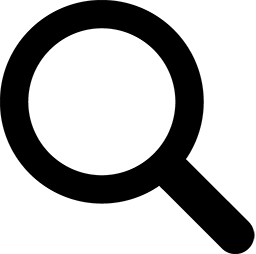
\includegraphics[scale=.02]{images/strm/magnify} 
    ~ ``Hurricane Sandy''};






\uncover<1>{
\node[anchor=north west,text width=12cm] at (5,7) {
\begin{itemize}
\item \large  Questions for designing a stream summarization model:
    \begin{itemize}
    \vspace{10pt}
\item \large How to increment system time?
    \vspace{10pt}
\item \large How to identify salience sentences?
    \vspace{10pt}
\item \large How to select updates?
    \end{itemize}

\end{itemize}
};
}

\uncover<2>{
\node[anchor=north west,text width=12cm] at (5,7) {

    We propose two models:

    \begin{itemize}
        \item Salience-biased Affinity Propagation (SAP) Summarizer
        \item Learning-to-Search (L2S) Summarizer
    \end{itemize}

\begin{tabular}{p{3.5cm}ll}
        \toprule
   & SAP Summarizer & L2S Summarizer \\
        \midrule
        How to increment system time? & Hourly increments & Fully-Online\\
        How to identify salience sentences? & Regression Model & \cellcolor[gray]{.95}\\
        How to select updates? & Clustering + Thresh.  &  \multirow{-2}{*}{\cellcolor[gray]{.95} Learned Policy} \\
        \bottomrule
    \end{tabular}

};
}
%\uncover<3->{
%\node[anchor=north west,text width=12cm] at (10,8) {
%    \textbf{SAP Summarizer}
%
%};
%
%}
 
   \node (b) at (5,5.25) {
       \begin{tikzpicture}[transform canvas={scale=0.4}]
           \tikzstyle{sent}=[align=left]
           \tikzstyle{doc}=[rectangle,rounded corners,draw=black, very thick]


%%% SUMMARIES

%           \visible<5->{  
%           \draw (-.02,5.5-1) node  [
%               very thick,weird fill=blue!10,
%               text width=0.15cm,align=center,text height=0.2cm
%            ] {};
%            \draw[doc] (-.25,5.75-1) rectangle (9.5, 5.25-1); 
%            \node[sent,left] at (9.5, 5.5-1) {\fontsize{7}{11}\selectfont 
%                \textbf{... two bombs went off at the finish line of the 
%                        Boston  Marathon.}};
% 
%            \draw (-.02,4.5-1) node  [
%                very thick,weird fill=blue!10,
%                text width=0.15cm,align=center,text height=0.2cm
%            ] {};
%            \draw[doc] (-.25,4.75-1) rectangle (9.5, 4.25-1); 
%            \node[sent,left] at (9.5, 4.5-1) {\fontsize{7}{11}\selectfont 
%                \textbf{Many of the injured were 
%                        reportedly bystanders.}};
%
%            \draw (-.02,3.5-1) node  [
%                very thick,weird fill=blue!10,
%                text width=0.15cm,align=center,text height=0.2cm
%            ] {};
%            \draw[doc] (-.25,3.75-1) rectangle (9.5, 3.25-1); 
%            \node[sent,left] at (9.5, 3.5-1) {\fontsize{7}{11}\selectfont 
%                \textbf{... two more explosive devices
%                        have been found.}};
%            \path[-,draw,very thick,orange,rounded corners] (2.3,3-1) -- 
%                (9.7,3-1) -- 
%                (9.7,6-1) -- (-.5,6-1)
%                -- (-.5,3-1) -- (2.3,3-1);
%            \node at (4,6.5-1) [] {\Huge Update Summary: 2pm -- 3pm};
%            }
%
%            \visible<6->{  
%            \draw ($(-.02,1.5)+(0,-4-1)$) node  [
%               very thick,weird fill=blue!10,
%               text width=0.15cm,align=center,text height=0.2cm
%            ] {};
%            \draw[doc] ($(-.25,1.75)+(0,-4-1)$) rectangle 
%                ($(9.5, 1.25)+(0,-4-1)$); 
%            \node[sent,left] at ($(9.5, 1.5)+(0,-4-1)$) {
%                \fontsize{7}{11}\selectfont 
%                \textbf{... two bombs went off at the finish line of the 
%                        Boston  Marathon.}};
% 
%            \draw ($(-.02,0.5)+(0,-4-1)$) node  [
%                very thick,weird fill=blue!10,
%                text width=0.15cm,align=center,text height=0.2cm
%            ] {};
%            \draw[doc] ($(-.25,0.75)+(0,-4-1)$) rectangle 
%                ($(9.5, 0.25)+(0,-4-1)$); 
%            \node[sent,left] at ($(9.5, 0.5)+(0,-4-1)$) {
%                \fontsize{7}{11}\selectfont 
%                \textbf{Many of the injured were 
%                        reportedly bystanders.}};
%
%            \draw ($(-.02,-0.5)+(0,-4-1)$) node  [
%                very thick,weird fill=blue!10,
%                text width=0.15cm,align=center,text height=0.2cm
%            ] {};
%            \draw[doc] ($(-.25,-0.25)+(0,-4-1)$) rectangle 
%                ($(9.5,-0.75)+(0,-4-1)$); 
%            \node[sent,left] at ($(9.5, -0.5)+(0,-4-1)$) {
%                \fontsize{7}{11}\selectfont 
%                \textbf{... two more explosive devices
%                        have been found.}};
%
%            \path[-,draw,orange,very thick,rounded corners] ($(2.3,3)+(0,-8-1)$) -- 
%                ($(9.7,3)+(0,-8-1)$) -- ($(9.7,6)+(0,-8-1)$) -- 
%                ($(-.5,6)+(0,-8-1)$) -- ($(-.5,3)+(0,-8-1)$) -- 
%                ($(2.3,3)+(0,-8-1)$);
%            \node at ($(4,6.5)+(0,-8-1)$) [] {\Huge Update Summary: 3pm -- 4pm};
%            }
%
%            \visible<7->{  
%            \draw ($(-.02,1.5)+(0,-11-1)$) node  [
%               very thick,weird fill=blue!10,
%               text width=0.15cm,align=center,text height=0.2cm
%            ] {};
%            \draw[doc] ($(-.25,1.75)+(0,-11-1)$) rectangle 
%                ($(9.5, 1.25)+(0,-11-1)$); 
%            \node[sent,left] at ($(9.5, 1.5)+(0,-11-1)$) {
%                \fontsize{7}{11}\selectfont 
%                \textbf{... two bombs went off at the finish line of the 
%                        Boston  Marathon.}};
% 
%            \draw ($(-.02,0.5)+(0,-11-1)$) node  [
%                very thick,weird fill=blue!10,
%                text width=0.15cm,align=center,text height=0.2cm
%            ] {};
%            \draw[doc] ($(-.25,0.75)+(0,-11-1)$) rectangle 
%                ($(9.5, 0.25)+(0,-11-1)$); 
%            \node[sent,left] at ($(9.5, 0.5)+(0,-11-1)$) {
%                \fontsize{7}{11}\selectfont 
%                \textbf{Many of the injured were 
%                        reportedly bystanders.}};
%
%            \draw ($(-.02,-0.5)+(0,-11-1)$) node  [
%                very thick,weird fill=blue!10,
%                text width=0.15cm,align=center,text height=0.2cm
%            ] {};
%            \draw[doc] ($(-.25,-0.25)+(0,-11-1)$) rectangle 
%                ($(9.5,-0.75)+(0,-11-1)$); 
%            \node[sent,left] at ($(9.5, -0.5)+(0,-11-1)$) {
%                \fontsize{7}{11}\selectfont 
%                \textbf{... two more explosive devices
%                        have been found.}};
%            \path[-,draw,orange,rounded corners,very thick] ($(2.3,3)+(0,-15-1)$) -- 
%                ($(9.7,3)+(0,-15-1)$) -- ($(9.7,6)+(0,-15-1)$) -- 
%                ($(-.5,6)+(0,-15-1)$) -- ($(-.5,3)+(0,-15-1)$) -- 
%                ($(2.3,3)+(0,-15-1)$);
%            \node at ($(4,6.5)+(0,-15-1)$) [] {\Huge Update Summary: 4pm -- 5pm};
%            }


  \end{tikzpicture}
  };


 
    \draw[white,top color=orange,bottom color=orange!20,shading=axis,
          shading angle=16] (0,2) -- (0,0) -- (1.7,0) -- 
            (1.7,2) -- (0,2) -- cycle; 
    \draw[white,top color=orange,bottom color=orange!20,shading=axis,
          shading angle=165] (0,5) -- (0,2) -- (.85,1) -- (1.7,2) -- 
            (1.7,5) -- (0,5) -- cycle; 

    \draw[white,top color=orange,bottom color=orange!20,shading=axis,
          shading angle=25] (0,8) -- (0,5) -- (0.85,4) -- (1.7,5) -- 
            (1.7,8) -- (0,8) -- cycle;
    \draw[white,top color=orange!90,bottom color=orange!20,shading=axis,
          shading angle=25] (0,8) -- (0.85,7) -- (1.7,8) -- (0,8) -- cycle;

    \node[rotate=90,text=white] at (.85,5.8) {\Huge 2:00};
    \node[rotate=90,text=white] at (.85,2.8) {\Huge 3:00};

  \node (f) at (2,6.55) {
  \begin{tikzpicture}[transform canvas={scale=0.2}]
    \tikzstyle{sent}=[align=left]
    \tikzstyle{doc}=[rectangle,rounded corners,draw=black, very thick]

    \draw (-.02,4.75) node  [
    very thick,
    weird fill=blue!10,
    text width=0.15cm,align=center,text height=1.8cm] {};
    \draw[doc] (-.25,5.80) rectangle (9.5, 3.70); 
    \node[sent,left] at (9.5, 5.5) {\fontsize{7}{11}\selectfont ... two bombs went off at the 
        finish line of the Boston  Marathon.};
    \node[sent,left] at (9.5, 5) {\fontsize{7}{11}\selectfont Many of the injured were 
        reportedly bystanders.};
    \node[sent,left] at (9.5, 4.5) {\fontsize{7}{11}\selectfont The blasts reportedly happened 
        across the street from the Lenox Hotel.};
    \node[sent,left] at (9.5, 4) {\fontsize{7}{11}\selectfont We will update you on any 
        breaking news we hear about this.};
    \node[rotate=90] at (0,4.75) {\tiny 3:05 pm} ;

    \draw (-.02,2.5) node  [
    very thick,
    weird fill=blue!10,
    text width=0.15cm,align=center,text height=1.3cm] {};
    \draw[doc] (-.25,3.30) rectangle (9.5, 1.70); 
    \node[sent,left] at (9.5, 3) {\fontsize{7}{11}\selectfont ... two bombs were detonated at 
        the race's finish line, killing and injuring many.};
    \node[sent,left] at (9.5, 2.5) {\fontsize{7}{11}\selectfont ... two more explosive devices
         have been found.};
    \node[sent,left] at (9.5, 2.0) {\fontsize{7}{11}\selectfont The White House says President 
        Obama has been notified about the explosions.};
    \node[rotate=90] at (0,2.5) {\tiny 3:45 pm} ;

    \draw (-.02,0.75) node  [
    very thick,
    weird fill=blue!10,
    text width=0.15cm,align=center,text height=0.8cm] {};
    \node[rotate=90] at (0,0.75) {\tiny 3:55 pm} ;
    \draw[doc] (-.25,1.30) rectangle (9.5,.2); 
    \node[sent,left] at (9.5, 1.0) {\fontsize{7}{11}\selectfont NBC news reports that 
        ``multiple explosive devices'' have been found in Boston.};
    \node[sent,left] at (9.5, 0.5) {\fontsize{7}{11}\selectfont Boston police report
        that two people were killed and at least 22 injured.};


  \end{tikzpicture}
  };
 \node (c) at (2,5.05) {
  \begin{tikzpicture}[transform canvas={scale=0.2}]
    \tikzstyle{sent}=[align=left]
    \tikzstyle{doc}=[rectangle,rounded corners,draw=black, very thick]


    \draw (-.02,6.75) node  [
    very thick,
    weird fill=blue!10,
    text width=0.15cm,align=center,text height=0.8cm] {};
    \draw[doc] (-.25,7.30) rectangle (9.5, 6.20); 
    \node[sent,left] at (9.5, 7) {\fontsize{7}{11}\selectfont Moments ago there were 
        explosions near the finish line of the Boston Marathon.}; 
    \node[sent,left] at (9.5, 6.5) {\fontsize{7}{11}\selectfont It has not been confirmed, 
        but its quite likely these were bombings.};
    \node[rotate=90] at (0,6.75) {\tiny 3:00 pm} ;
    
    \draw (-.02,4.75) node  [
    very thick,
    weird fill=blue!10,
    text width=0.15cm,align=center,text height=1.8cm] {};
    \draw[doc] (-.25,5.80) rectangle (9.5, 3.70); 
    \node[sent,left] at (9.5, 5.5) {\fontsize{7}{11}\selectfont ... two bombs went off at the 
        finish line of the Boston  Marathon.};
    \node[sent,left] at (9.5, 5) {\fontsize{7}{11}\selectfont Many of the injured were 
        reportedly bystanders.};
    \node[sent,left] at (9.5, 4.5) {\fontsize{7}{11}\selectfont The blasts reportedly happened 
        across the street from the Lenox Hotel.};
    \node[sent,left] at (9.5, 4) {\fontsize{7}{11}\selectfont We will update you on any 
        breaking news we hear about this.};
    \node[rotate=90] at (0,4.75) {\tiny 3:05 pm} ;

    \draw (-.02,2.5) node  [
    very thick,
    weird fill=blue!10,
    text width=0.15cm,align=center,text height=1.3cm] {};
    \draw[doc] (-.25,3.30) rectangle (9.5, 1.70); 
    \node[sent,left] at (9.5, 3) {\fontsize{7}{11}\selectfont ... two bombs were detonated at 
        the race's finish line, killing and injuring many.};
    \node[sent,left] at (9.5, 2.5) {\fontsize{7}{11}\selectfont ... two more explosive devices
         have been found.};
    \node[sent,left] at (9.5, 2.0) {\fontsize{7}{11}\selectfont The White House says President 
        Obama has been notified about the explosions.};
    \node[rotate=90] at (0,2.5) {\tiny 3:45 pm} ;

    \draw (-.02,0.75) node  [
    very thick,
    weird fill=blue!10,
    text width=0.15cm,align=center,text height=0.8cm] {};
    \node[rotate=90] at (0,0.75) {\tiny 3:55 pm} ;
    \draw[doc] (-.25,1.30) rectangle (9.5,.2); 
    \node[sent,left] at (9.5, 1.0) {\fontsize{7}{11}\selectfont NBC news reports that 
        ``multiple explosive devices'' have been found in Boston.};
    \node[sent,left] at (9.5, 0.5) {\fontsize{7}{11}\selectfont Boston police report
        that two people were killed and at least 22 injured.};


  \end{tikzpicture}
  };

  \node (a) at (2,3.5) {
  \begin{tikzpicture}[transform canvas={scale=0.2}]
    \tikzstyle{sent}=[align=left]
    \tikzstyle{doc}=[rectangle,rounded corners,draw=black, very thick]

    \draw[black,rounded corners,very thick,dotted] (-0.5,7.5) rectangle (9.75,0);

    \draw (-.02,6.75) node  [
    very thick,
    weird fill=blue!10,
    text width=0.15cm,align=center,text height=0.8cm] {};
    \draw[doc] (-.25,7.30) rectangle (9.5, 6.20); 
    \node[sent,left] at (9.5, 7) {\fontsize{7}{11}\selectfont Moments ago there were 
        explosions near the finish line of the Boston Marathon.}; 
    \node[sent,left] at (9.5, 6.5) {\fontsize{7}{11}\selectfont It has not been confirmed, 
        but its quite likely these were bombings.};
    \node[rotate=90] at (0,6.75) {\tiny 3:00 pm} ;
    
    \draw (-.02,4.75) node  [
    very thick,
    weird fill=blue!10,
    text width=0.15cm,align=center,text height=1.8cm] {};
    \draw[doc] (-.25,5.80) rectangle (9.5, 3.70); 
    \node[sent,left] at (9.5, 5.5) {\fontsize{7}{11}\selectfont ... two bombs went off at the 
        finish line of the Boston  Marathon.};
    \node[sent,left] at (9.5, 5) {\fontsize{7}{11}\selectfont Many of the injured were 
        reportedly bystanders.};
    \node[sent,left] at (9.5, 4.5) {\fontsize{7}{11}\selectfont The blasts reportedly happened 
        across the street from the Lenox Hotel.};
    \node[sent,left] at (9.5, 4) {\fontsize{7}{11}\selectfont We will update you on any 
        breaking news we hear about this.};
    \node[rotate=90] at (0,4.75) {\tiny 3:05 pm} ;

    \draw (-.02,2.5) node  [
    very thick,
    weird fill=blue!10,
    text width=0.15cm,align=center,text height=1.3cm] {};
    \draw[doc] (-.25,3.30) rectangle (9.5, 1.70); 
    \node[sent,left] at (9.5, 3) {\fontsize{7}{11}\selectfont ... two bombs were detonated at 
        the race's finish line, killing and injuring many.};
    \node[sent,left] at (9.5, 2.5) {\fontsize{7}{11}\selectfont ... two more explosive devices
         have been found.};
    \node[sent,left] at (9.5, 2.0) {\fontsize{7}{11}\selectfont The White House says President 
        Obama has been notified about the explosions.};
    \node[rotate=90] at (0,2.5) {\tiny 3:45 pm} ;

    \draw (-.02,0.75) node  [
    very thick,
    weird fill=blue!10,
    text width=0.15cm,align=center,text height=0.8cm] {};
    \node[rotate=90] at (0,0.75) {\tiny 3:55 pm} ;
    \draw[doc] (-.25,1.30) rectangle (9.5,.2); 
    \node[sent,left] at (9.5, 1.0) {\fontsize{7}{11}\selectfont NBC news reports that 
        ``multiple explosive devices'' have been found in Boston.};
    \node[sent,left] at (9.5, 0.5) {\fontsize{7}{11}\selectfont Boston police report
        that two people were killed and at least 22 injured.};


  \end{tikzpicture}
  };

 \node (d) at (2,2.00) {
  \begin{tikzpicture}[transform canvas={scale=0.2}]
    \tikzstyle{sent}=[align=left]
    \tikzstyle{doc}=[rectangle,rounded corners,draw=black, very thick]


    \draw (-.02,6.75) node  [
    very thick,
    weird fill=blue!10,
    text width=0.15cm,align=center,text height=0.8cm] {};
    \draw[doc] (-.25,7.30) rectangle (9.5, 6.20); 
    \node[sent,left] at (9.5, 7) {\fontsize{7}{11}\selectfont Moments ago there were 
        explosions near the finish line of the Boston Marathon.}; 
    \node[sent,left] at (9.5, 6.5) {\fontsize{7}{11}\selectfont It has not been confirmed, 
        but its quite likely these were bombings.};
    \node[rotate=90] at (0,6.75) {\tiny 3:00 pm} ;
    
    \draw (-.02,4.75) node  [
    very thick,
    weird fill=blue!10,
    text width=0.15cm,align=center,text height=1.8cm] {};
    \draw[doc] (-.25,5.80) rectangle (9.5, 3.70); 
    \node[sent,left] at (9.5, 5.5) {\fontsize{7}{11}\selectfont ... two bombs went off at the 
        finish line of the Boston  Marathon.};
    \node[sent,left] at (9.5, 5) {\fontsize{7}{11}\selectfont Many of the injured were 
        reportedly bystanders.};
    \node[sent,left] at (9.5, 4.5) {\fontsize{7}{11}\selectfont The blasts reportedly happened 
        across the street from the Lenox Hotel.};
    \node[sent,left] at (9.5, 4) {\fontsize{7}{11}\selectfont We will update you on any 
        breaking news we hear about this.};
    \node[rotate=90] at (0,4.75) {\tiny 3:05 pm} ;

    \draw (-.02,2.5) node  [
    very thick,
    weird fill=blue!10,
    text width=0.15cm,align=center,text height=1.3cm] {};
    \draw[doc] (-.25,3.30) rectangle (9.5, 1.70); 
    \node[sent,left] at (9.5, 3) {\fontsize{7}{11}\selectfont ... two bombs were detonated at 
        the race's finish line, killing and injuring many.};
    \node[sent,left] at (9.5, 2.5) {\fontsize{7}{11}\selectfont ... two more explosive devices
         have been found.};
    \node[sent,left] at (9.5, 2.0) {\fontsize{7}{11}\selectfont The White House says President 
        Obama has been notified about the explosions.};
    \node[rotate=90] at (0,2.5) {\tiny 3:45 pm} ;

    \draw (-.02,0.75) node  [
    very thick,
    weird fill=blue!10,
    text width=0.15cm,align=center,text height=0.8cm] {};
    \node[rotate=90] at (0,0.75) {\tiny 3:55 pm} ;
    \draw[doc] (-.25,1.30) rectangle (9.5,.2); 
    \node[sent,left] at (9.5, 1.0) {\fontsize{7}{11}\selectfont NBC news reports that 
        ``multiple explosive devices'' have been found in Boston.};
    \node[sent,left] at (9.5, 0.5) {\fontsize{7}{11}\selectfont Boston police report
        that two people were killed and at least 22 injured.};


  \end{tikzpicture}
  };

\node (e) at (2,0.2) {
  \begin{tikzpicture}[transform canvas={scale=0.2}]
    \tikzstyle{sent}=[align=left]
    \tikzstyle{doc}=[rectangle,rounded corners,draw=black, very thick]

    \draw (-.02,8.25) node  [
    very thick,
    weird fill=blue!10,
    text width=0.15cm,align=center,text height=0.8cm] {};
    \draw[doc] (-.25,8.8) rectangle (9.5, 7.70); 
    \node[sent,left] at (9.5, 8.5) {\fontsize{7}{11}\selectfont Moments ago there were 
        explosions near the finish line of the Boston Marathon.}; 
    \node[sent,left] at (9.5, 8) {\fontsize{7}{11}\selectfont It has not been confirmed, 
        but its quite likely these were bombings.};
    \node[rotate=90] at (0,8.25) {\tiny 3:00 pm} ;
 
    \draw (-.02,6.75) node  [
    very thick,
    weird fill=blue!10,
    text width=0.15cm,align=center,text height=0.8cm] {};
    \draw[doc] (-.25,7.30) rectangle (9.5, 6.20); 
    \node[sent,left] at (9.5, 7) {\fontsize{7}{11}\selectfont Moments ago there were 
        explosions near the finish line of the Boston Marathon.}; 
    \node[sent,left] at (9.5, 6.5) {\fontsize{7}{11}\selectfont It has not been confirmed, 
        but its quite likely these were bombings.};
    \node[rotate=90] at (0,6.75) {\tiny 3:00 pm} ;
    
    \draw (-.02,4.75) node  [
    very thick,
    weird fill=blue!10,
    text width=0.15cm,align=center,text height=1.8cm] {};
    \draw[doc] (-.25,5.80) rectangle (9.5, 3.70); 
    \node[sent,left] at (9.5, 5.5) {\fontsize{7}{11}\selectfont ... two bombs went off at the 
        finish line of the Boston  Marathon.};
    \node[sent,left] at (9.5, 5) {\fontsize{7}{11}\selectfont Many of the injured were 
        reportedly bystanders.};
    \node[sent,left] at (9.5, 4.5) {\fontsize{7}{11}\selectfont The blasts reportedly happened 
        across the street from the Lenox Hotel.};
    \node[sent,left] at (9.5, 4) {\fontsize{7}{11}\selectfont We will update you on any 
        breaking news we hear about this.};
    \node[rotate=90] at (0,4.75) {\tiny 3:05 pm} ;

    \draw (-.02,2.5) node  [
    very thick,
    weird fill=blue!10,
    text width=0.15cm,align=center,text height=1.3cm] {};
    \draw[doc] (-.25,3.30) rectangle (9.5, 1.70); 
    \node[sent,left] at (9.5, 3) {\fontsize{7}{11}\selectfont ... two bombs were detonated at 
        the race's finish line, killing and injuring many.};
    \node[sent,left] at (9.5, 2.5) {\fontsize{7}{11}\selectfont ... two more explosive devices
         have been found.};
    \node[sent,left] at (9.5, 2.0) {\fontsize{7}{11}\selectfont The White House says President 
        Obama has been notified about the explosions.};
    \node[rotate=90] at (0,2.5) {\tiny 3:45 pm} ;

    \draw (-.02,0.75) node  [
    very thick,
    weird fill=blue!10,
    text width=0.15cm,align=center,text height=0.8cm] {};
    \node[rotate=90] at (0,0.75) {\tiny 3:55 pm} ;
    \draw[doc] (-.25,1.30) rectangle (9.5,.2); 
    \node[sent,left] at (9.5, 1.0) {\fontsize{7}{11}\selectfont NBC news reports that 
        ``multiple explosive devices'' have been found in Boston.};
    \node[sent,left] at (9.5, 0.5) {\fontsize{7}{11}\selectfont Boston police report
        that two people were killed and at least 22 injured.};


  \end{tikzpicture}
  };

%    \visible<5>{
%        \node (BOX) at (2.95,6.45) [
%            draw,rectangle,minimum width=2.2cm,
%            minimum height=2.8cm,very thick,orange,
%            rounded corners] {};
%
%    \node (T1) at ($(BOX.south east)+(0.25,0)$) {$\quad\tau_i$};
%    \draw[-,line width=0.5mm] ($(BOX.south east)+(0.25,-0.1)$) -- ($(BOX.south west)+(-0.2,-0.1)$);
%    }
%    \visible<6>{
%        \node (BOX) at (2.95,3.5) [
%            draw,rectangle,minimum width=2.2cm,
%            minimum height=3cm,very thick,orange,
%            rounded corners] {};
%            \node (T1) at ($(BOX.south east)+(0.25,0)$) {$\quad\tau_{i+1}$};
%    \draw[-,line width=0.5mm] ($(BOX.south east)+(0.25,-0.1)$) -- ($(BOX.south west)+(-0.2,-0.1)$);
%    }
%    \visible<7>{
%        \node (BOX) at (2.95,1.1) [
%            draw,rectangle,minimum width=2.2cm,
%            minimum height=1.8cm,very thick,orange,
%            rounded corners] {};
%            \node (T1) at ($(BOX.south east)+(0.25,0)$) {$\quad\tau_{i+2}$};
%    \draw[-,line width=0.5mm] ($(BOX.south east)+(0.25,-0.1)$) -- ($(BOX.south west)+(-0.2,-0.1)$);
%    }
%    \visible<6>{
%        \node at (2.95,6.45) [
%            draw,rectangle,minimum width=2.2cm,
%            minimum height=2.8cm,very thick,white,fill=white,
%            rounded corners,opacity=.8] {};
%
%        \node at (2.95,1.1) [
%            draw,rectangle,minimum width=2.2cm,
%            minimum height=1.8cm,very thick,white,fill=white,
%            rounded corners,opacity=.8] {};
%
%        \node at (2.95,4.85) [
%            draw,rectangle,minimum width=2.2cm,
%            minimum height=.25cm,very thick,orange,
%            rounded corners] {};
%    }

 
    \end{tikzpicture}}
%%% ANCHOR
\end{frame}

\begin{frame}{SAP}

    \begin{itemize}
        \item Salience Model 
    \begin{itemize}
        \item regression model $f(\phi(s))$
        \item trained to predict the maximum semantic similarity of 
            a sentence $s$ to the query nuggets $\mathcal{N}$,
        $\max_{n \in \mathcal{N}} \operatorname{sim}(n, s) = f(\phi(s))$.

%    \item $\phi(s)$ -- feature function of $s$ 
%    \item $\operatorname{sim}(n,s)= \operatorname{cos-sim}(\psi(n),\psi(s))$ -- cosine similarity between dense, low-dimensional projection $\psi$ of the 
%        tf-idf weighted bag-of-words represenatation of $n$ and $s$. (Srebro \& Jaakkola, 2003; Guo \& Diab, 2012)


    \end{itemize}
    \vspace{10pt}
\item Update Selection
    \begin{itemize}
        \item Salience estimates used to bias cluster formation in 
            Affinity Propogation algorithm.
        \item Salience-biased Affinity Propogation identifies candidate updates.
        \item Candidates added to the update summary if their similarity to
            previous updates is below a threshold.
    \end{itemize}

    \end{itemize}

\end{frame}

\begin{frame}{L2S}

    \begin{itemize}
        \item SAP model must wait to cache enough documents to perform clustering.
            \vspace{10pt}
        \item With the L2S model, we learn a greedy policy for making extraction decisions immediately as new documents come in.
            \vspace{10pt}
        \item The policy, $\pi(\phi(s))$, learns to make extraction decisions using Locally-Optimal Learning-to-Search (LOLS) paradigm (Chang et al., 2015)

    \end{itemize}

\end{frame}

\begin{frame}{Sentence Features $\phi(s)$ }

\begin{columns}
\begin{column}{0.5\textwidth}
\begin{itemize}

    \item Non-Content Features (e.g., position/length)
\item Query Relevance Features
\item Language Model Scores 
\item Geographic Features
\item Temporal Features
\end{itemize}
\end{column}
\begin{column}{0.5\textwidth}
    \textbf{L2S additional features}
\begin{itemize}
\item Update Similarity
\item Single Document Summarization Rankings
\item Nugget Probability
\item Stream Language Models
\item Stream Document Frequency
\item Feature Interactions 

\end{itemize}
\end{column}
\end{columns}

\end{frame}

\begin{frame}{Metrics}
\begin{itemize}
\item Expected Gain  --- (Nugget Precision) 
 average number of novel nuggets matched to each update

\vspace{10pt}
\item Comprehensiveness --- (Nugget Recall) percent of unique nuggets matched
by update summary
\vspace{10pt}
\item F1 --- Harmonic Mean of Expected Gain and Comprehensiveness

\vspace{10pt}
\item Latency Weighted variants of the above metrics
\begin{itemize}
\item Value of each nugget match decreases to 0 if it is extracted after its reference time.
\item Value of each nugget match increases to as much as 2 if it is 
extracted before its reference time.
\end{itemize}

\end{itemize}


\end{frame}


\begin{frame}{Evaluations}

\begin{itemize}
\item Temporal Summarization Shared-Tasks at TREC 2014 
\begin{itemize}
\item Submitted SAP.
\end{itemize}
\item Temporal Summarization Shared-Tasks at TREC 2015
\begin{itemize}
\item Submitted L2S, and SAP.
\end{itemize}
\vspace{10pt}
\item Performed our own automatic $k$-fold evaluations of SAP and L2S summarizers. 
\end{itemize}
\end{frame}

\begin{frame}{TREC 2014 Evaluation}
\begin{columns}
\begin{column}{0.5\textwidth}
\begin{itemize}
\item SAP was \textbf{first} in overall metric, latency weighted F1 
\vspace{10pt}
\item SAP increases Expected Gain over AP-Clustering only baseline.
\vspace{10pt}
\item SAP had \begin{itemize}
\item above average Expected Gain, 
\item slightly below average Comprehensiveness, 
\item better latency than the top 3 highest Expected Gain runs, 
\end{itemize}
\end{itemize}
\end{column}
\begin{column}{0.5\textwidth}
\begin{tikzpicture}
\node at (0,0) {\resizebox{0.70\textwidth}{!}{
\begin{tabular}{cccccc}
\toprule
TeamID & RunID &Exp. Gain & Comp. & Comp. (Latency) & F1 (Latency) \\
\midrule
\textbf{cunlp} & \textbf{2SAP} & 0.0631 & 0.3220 & 1.2068 & \textbf{0.1162} \\
BJUT & Q1 & \textbf{0.0657} & 0.4088 & 1.1491 & 0.1110\\
BJUT & Q2 & 0.0632 & 0.3979 & 1.1669 & 0.1091\\
BJUT & Q0 & 0.0632 & 0.3979 & 1.1669 & 0.1091\\
uogTr & uogTr2A & 0.0467 & 0.4453 & 1.2322 & 0.0986\\
uogTr & uogTr4AC & 0.0347 & 0.4539 & 1.2751 & 0.0793\\
uogTr & uogTr4ARas & 0.0387 & 0.3691 & 1.2328 & 0.0772\\
IRIT & KW30H5NW3600 & 0.0383 & 0.3521 & 1.2221 & 0.0723\\
IRIT & KW30H5NW300 & 0.0378 & 0.3538 & 1.2208 & 0.0714\\
uogTr & uogTr4A & 0.0281 & \textbf{0.4733} & 1.2522 & 0.0677\\
\midrule
\multicolumn{2}{c}{\textit{average}} & 0.0327 & 0.3615 & 1.2943 & 0.0620\\
\midrule
IRIT & KW80H5NW3600 & 0.0289 & 0.3764 & 1.2191 & 0.0604\\
IRIT & KW30H10NW300 & 0.0298 & 0.3780 & 1.2617 & 0.0602\\
cunlp & 1APSalRed & 0.0325 & 0.3058 & 1.1507 & 0.0602\\
IRIT & KW80H5NW300 & 0.0285 & 0.3806 & 1.2164 & 0.0596\\
ICTNET & run3 & 0.0531 & 0.1081 & 0.7004 & 0.0530\\
BUPT\_PRIS & Cluster4 & 0.0155 & 0.2692 & 1.9140 & 0.0508\\
IRIT & KW80H10NW300 & 0.0225 & 0.4012 & 1.2621 & 0.0503\\
BUPT\_PRIS & Cluster3 & 0.0115 & 0.3380 & 1.9165 & 0.0407\\
\textbf{cunlp} & \textbf{3AP} & 0.0174 & 0.4265 & 1.3689 & 0.0403\\
ICTNET & run2 & 0.0418 & 0.0934 & 0.6266 & 0.0311\\
BUPT\_PRIS & Cluster2 & 0.0059 & 0.3728 & 1.9170 & 0.0222\\
ICTNET & run4 & 0.0079 & 0.4070 & 1.2364 & 0.0178\\
ICTNET & run1 & 0.0070 & 0.4090 & 1.2314 & 0.0160\\
BUPT\_PRIS & Cluster1 & 0.0033 & 0.4369 & \textbf{1.9175} & 0.0127\\
\bottomrule
\end{tabular}}};
\node (e2) at (-2.25,2.05) {};
\node (s2) at (-3,2.05) {};
\node (e1) at (-2.25,-1.4) {};
\node (s1) at (-3,-1.4) {};
\draw[line width=0.7mm,->] (s1) -- (e1);
\draw[line width=0.7mm,->] (s2) -- (e2);
\node  at ($(s1.north)!0.5!(e1.north)+(0,0.15)$) {\large \textbf{AP}};
\node  at ($(s2.north)!0.5!(e2.north)+(0,0.15)$) {\large \textbf{SAP}};
\end{tikzpicture}
\end{column}
\end{columns}

\end{frame}

\begin{frame}{Automatic \textsc{Rouge} Evaluation}
\begin{columns}
\begin{column}{0.5\textwidth}
    \begin{tikzpicture}
        \node at (0,0) {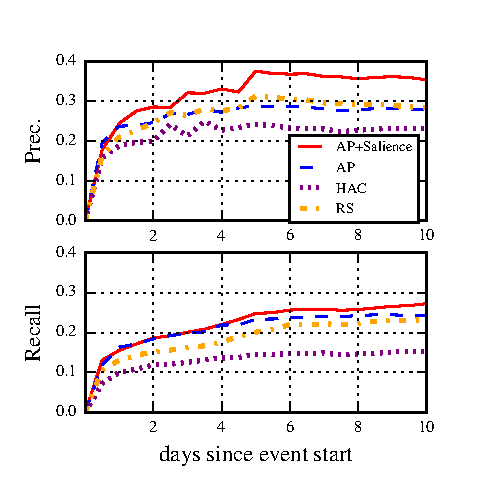
\includegraphics[]{images/strm/rouge-time.eps}};
        \node[draw=white,fill=white,text width=1.05cm] at (2.20,1.55) {};
        \node[draw=white,fill=white,inner sep=0pt,text width=1.05cm] at (2.20,1.60) {\tiny SAP};
        \node[draw=white,fill=white,text width=1.05cm] at (2.20,1.30) {};
        \node[draw=white,fill=white,text width=1.05cm] at (2.20,0.95) {};
        \node[draw=white,fill=white,text width=1.05cm] at (2.20,0.55) {};

        \node[draw=white,fill=white,inner sep=0pt,text width=1.05cm] at (2.20,1.25) {\tiny AP};
        \node[draw=white,fill=white,inner sep=0pt,text width=1.05cm] at (2.20,0.90) {\tiny HAC};
        \node[draw=white,fill=white,inner sep=0pt,text width=1.05cm] at (2.20,0.55) {\tiny RS};
    \end{tikzpicture}
\end{column}
\begin{column}{0.5\textwidth}
\begin{itemize}
\item SAP achieves higher \textsc{Rouge}-1 precision faster than baselines
\vspace{10pt}

\end{itemize}
\end{column}
\end{columns}

\end{frame}


\begin{frame}{Automatic Rouge Evaluation}
    \begin{columns}
        \begin{column}{0.5\textwidth}
            \begin{center}
    \begin{tabular}{l c c }
            \toprule
        Model & \multicolumn{2}{c}{\textsc{Rouge}-1 F1} \\
                \midrule
        Full System & 0.306 \\
                \midrule
                No Simple  &  0.294 & \small (-.012)\\ 
                No Query &  0.280 & \alert<1>{\small (-.026)}\\ 
                No Geo   &  0.265 &\alert<1>{\small (-.041)}\\ 
                No LM     &  0.254 &\alert<1,2>{\small (-.052)}\\
                \midrule
                AP only  &  0.263 & \alert<2>{\small (-.043)} \\
                \bottomrule
            \end{tabular}
            \end{center}
        \end{column}
        \begin{column}{0.5\textwidth}
            
            \begin{itemize}
                \item Content features are more important than heuristics like position.

                \item<2-> Removing LM is worse than having no salience estimation.

            \end{itemize}

        \end{column}
    \end{columns}

\end{frame}


\begin{frame}{TREC 2015 Evaluation}
\begin{columns}
\begin{column}{0.5\textwidth}
\begin{itemize}
    \item L2S was \textbf{4th and 5th}, SAP was \textbf{7th} in overall metric, latency weighted F1 
\vspace{10pt}
\item L2S and SAP runs above average
\vspace{10pt}
\item L2S improves over SAP on all metrics
\end{itemize}
\end{column}
\begin{column}{0.5\textwidth}
\begin{tikzpicture}
\node at (0,0) {\resizebox{0.90\textwidth}{!}{
\begin{tabular}{cccccc}
\toprule
Team ID & Run ID & Expected Gain & Comp. & Comp. (Latency) & F1 (Latency) \\
\midrule
WaterlooClarke & UWCTSRun1 & 0.2350 & 0.3520 & 0.6612 & \textbf{0.1762}\\
WaterlooClarke & UWCTSRun3 & 0.2252 & 0.3421 & \textbf{0.6643} & 0.1718\\
WaterlooClarke & UWCTSRun2 & \textbf{0.2872} & 0.2584 & 0.6551 & 0.1710\\
\textbf{cunlp} & \textbf{3LtoSfltr5} & 0.1371 & 0.4870 & 0.6392 & 0.1282\\
\textbf{cunlp} & \textbf{1LtoSfltr20} & 0.1203 & 0.5372 & 0.6287 & 0.1100\\
IRIT & FS1A & 0.0849 & 0.4959 & 0.6051 & 0.0719\\
\textbf{cunlp} & \textbf{4SAP} & 0.1011 & 0.4584 & 0.5108 & 0.0674\\
\midrule
\multicolumn{2}{c}{\textit{average}} & 0.0666 & 0.4342 & 0.4697 & 0.0499\\
\midrule
IRIT & FS2A & 0.0518 & 0.5899 & 0.6285 & 0.0476\\
BJUT & DMSL1NMF2 & 0.0445 & 0.6123 & 0.4539 & 0.0354\\
BJUT & DMSL1AP1 & 0.0413 & \textbf{0.6155} & 0.4701 & 0.0338\\
l3sattrec15 & l3sattrec15run1 & 0.0408 & 0.3612 & 0.3743 & 0.0268\\
l3sattrec15 & l3sattrec15run3 & 0.0400 & 0.3669 & 0.3712 & 0.0262\\
IRIT & FS1B & 0.0422 & 0.2939 & 0.3913 & 0.0259\\
IRIT & FS2B & 0.0306 & 0.3391 & 0.4491 & 0.0239\\
USI & InL2DecrQE1ID1 & 0.0182 & 0.5713 & 0.5806 & 0.0196\\
USI & InL2DecrQE2ID2 & 0.0169 & 0.5758 & 0.5836 & 0.0184\\
udel\_fang & WikiOnlyFS2 & 0.0206 & 0.5819 & 0.4600 & 0.0176\\
udel\_fang & ProfOnlyFS3 & 0.0258 & 0.5294 & 0.4122 & 0.0174\\
USI & InL2StabQE2ID3 & 0.0171 & 0.6133 & 0.5238 & 0.0170\\
udel\_fang & WikiProfMixFS1 & 0.0189 & 0.5965 & 0.4660 & 0.0166\\
l3sattrec15 & l3sattrec15run2 & 0.0283 & 0.2276 & 0.2560 & 0.0164\\
USI & InL2IncrQE2ID4 & 0.0179 & 0.5837 & 0.2888 & 0.0108\\
\bottomrule
\end{tabular}}
};
\node (e2) at (-3.0,1.65) {};
\node (s2) at (-3.75,1.65) {};
\node (e1) at (-3.00,0.95) {};
\node (s1) at (-3.75,0.95) {};
\draw[line width=0.7mm,->] (s1) -- (e1);
\draw[line width=0.7mm,->] (s2) -- (e2);
\node  at ($(s1.north)!0.5!(e1.north)+(0,0.15)$) {\large \textbf{SAP}};
\node  at ($(s2.north)!0.5!(e2.north)+(0,0.15)$) {\large \textbf{L2S}};
\end{tikzpicture}
\end{column}
\end{columns}

\end{frame}


\begin{frame}{Automatic Evaluation}
    \begin{center}
\resizebox{0.5\textwidth}{!}{
\begin{tabular}{ l   c  c }
\toprule
%   &\multicolumn{3}{c}{unpenalized}&\multicolumn{3}{c}{latency-penalized}&\\
% \cmidrule(lr){2-4} \cmidrule(lr){5-7}
%   &
Model  & Nugget  F1 & Nugget F1 (latency) \\ % & Num. Updates \\
    \midrule
%\textsc{AP}         
%    & $0.083$            & $0.09$                     & $0.078$ 
%    & $0.079$            & $0.095$                    & $0.077$ 
%    & ~~$20.846$ \\
\textsc{SAP}      
& $0.094$ & \alert<2>{$0.088$} \\
   % & ~~~~$8.333$ \\
%\textsc{Cos}     
 %   & $0.075$            & $0.176$              & $0.099$ 
 %   & $0.095$            & $0.236$              & $0.128$ 
 %   & $145.615$ \\
\textsc{L2S}    &  ${\bf0.112}$  & \alert<3>{${\bf0.162}$} \\
   % & ~~$89.872$ \\
%\textsc{L2S-Cos}
%    & $0.115$        & $0.189$ & ${\bf0.127}$
%    & ${\bf0.162}$ & $0.276$ & ${\bf0.184}$
% & ~~$29.231$ \\
\bottomrule
\end{tabular}}
\end{center}

%\resizebox{\textwidth}{!}{
%\begin{tabular}{ l   c c c   c c c  c }
%\toprule
%   &\multicolumn{3}{c}{unpenalized}&\multicolumn{3}{c}{latency-penalized}&\\
% \cmidrule(lr){2-4} \cmidrule(lr){5-7}
%   & Exp. Gain     & Comp. 
%        & F1 & Exp. Gain     & Comp& F1 \\ % & Num. Updates \\
%    \bottomrule
%%\textsc{AP}         
%%    & $0.083$            & $0.09$                     & $0.078$ 
%%    & $0.079$            & $0.095$                    & $0.077$ 
%%    & ~~$20.846$ \\
%\textsc{SAP}      
%    & \alert<2>{$\mathbf{0.119}$} & $0.09$                     & $0.094$ 
%    & $0.105$            & $0.088$                    & $0.088$ \\
%   % & ~~~~$8.333$ \\
%%\textsc{Cos}     
% %   & $0.075$            & $0.176$              & $0.099$ 
% %   & $0.095$            & $0.236$              & $0.128$ 
% %   & $145.615$ \\
%\textsc{L2S}       
%    & $0.097$            & \alert<3>{$\mathbf{0.207}$}   & \alert<3>{${\bf0.112}$ }
%    & \alert<4>{${\bf0.136}$}      & \alert<4>{$\mathbf{0.306}$} & \alert<4>{${\bf0.162}$} \\
%   % & ~~$89.872$ \\
%%\textsc{L2S-Cos}
%%    & $0.115$        & $0.189$ & ${\bf0.127}$
%%    & ${\bf0.162}$ & $0.276$ & ${\bf0.184}$
%% & ~~$29.231$ \\
%\bottomrule
%\end{tabular}}}

\begin{itemize}
\item<2-> SAP was retrieving nuggets after the reference time, getting a latency penalty.
\item<3-> L2S beat reference times, getting a latency reward!

\end{itemize}
\end{frame}

\begin{frame}{L2S and Position Heuristics}

\begin{center}
  \begin{tabular}{ l   c c c  }
\toprule
    &\multicolumn{3}{c}{latency-penalized}\\
\cmidrule(lr){2-4}
    & Exp. Gain    & Comp. & F1 \\
    \midrule
  %  \textsc{Cos}  & $0.095$ & $\mathbf{0.236}$ & $0.128$ \\
     \textsc{L2S}  & $0.136$ & \alert{$0.306$} & $0.162$ \\
     \textsc{L2S-FS}  & $0.164$ & \alert{$0.220$} & $0.157$ \\
%    \textsc{L2S-Cos-FS} &
 %     $\mathbf{0.207}$ & $0.18~~$ & $\mathbf{0.163}$ \\
\bottomrule
  \end{tabular}
\end{center}

\begin{itemize}
\item L2S-FS (limited to first sentences) misses out on information in the body
\item<2> A good content model of salience is neccessary to find information in the body.
\end{itemize}


\end{frame}

\begin{frame}{Takeaways}

 We proposed two summarization models for query focused, news-stream summarization.
\begin{itemize}
                    \item SAP model -- Combines salience estimation + AP clustering.
\vspace{5pt}

                    \item L2S model -- greedy online summarizer, identifies salient information more quicly than SAP/baselines.

\vspace{5pt}
                    \item We denomstrate the importance of content features 
when modeling salience in this environment.
                \end{itemize}




\end{frame}




%%% 
%%% 
%%% \section{Faithful and Controllable Generation}
%%% 
%%% 
%\begin{frame}{Faithfulness Generation}
%
%
%    \begin{itemize}
%
%        \item<1-> \textbf{Faithfulness} \\ Output should respect the semantics of the input.
%
%~\\
%
%        \item<2->  \textbf{Control} \\
%            Surface realization/discourse planning are explicit parts of the
%            model.
%
%    \end{itemize}
%\end{frame}

\begin{frame}{Faithful Generation}

\begin{itemize}

        \item \textbf{Faithfulness} Output should respect the semantics of the input. 
\vspace{20pt}
\item Studying faithfulness in  end-to-end abstractive summarization models
is difficult, hard to attribute errors to decoder language model vs world knowledge
\vspace{20pt}
\item We use the meaning representation to text generation task
as an idealized setting to study these issues.
\end{itemize}

\end{frame}

\subsection{Task}

\begin{frame}{Meaning Representation-to-Text Generation}
  \begin{center}\begin{tikzpicture}

    %%% MR Display %%%
    \node[anchor=north west] at (0,1.0)
        {\large \textbf{Input: Meaning Representation (MR)}};    
    \only<1-5>{
        \node[anchor=north west] (mr) at (0,0) 
            {$\left[\!\!\!\left[ \begin{array}{l} 
                \textscorig{Inform} \\ 
                \textrm{name=Aromi} \\ 
                \textrm{eat\_type=coffee shop} \\ 
                \textrm{area=city centre} \\ 
            \end{array}\right]\!\!\!\right]$  };        
    }
    \only<6>{
        \node[anchor=north west] (mr) at (0,0) 
            {$\left[\!\!\!\left[ \begin{array}{l} 
                \textsc{Inform} \\ 
                \textbf{\color{Red}name=Aromi} \\ 
                \textbf{\color{Green}eat\_type=coffee shop} \\ 
                \textbf{\color{Blue}area=city centre} \\ 
            \end{array}\right]\!\!\!\right]$  };        
    }

    %%% Utterance Display %%%
    \uncover<2>{
        \draw[line width=0.75mm,->] (2.4,-2.5) -- (2.4,-3.5);

        \node[anchor=north west,align=left,draw=black,dotted] 
                (out) at (0,-4.0) 
            {   
                \large  
                \textbf{Output: Natural Language Utterance}\\~\\
                \Large\textit{For coffee in the city centre, try Aromi.}
            };  
    }
    \uncover<6>{
        \draw[line width=0.75mm,->] (2.4,-2.5) -- (2.4,-3.5);

        \node[anchor=north west,align=left,draw=black,dotted] 
                (out) at (0,-4.0) 
            {
                \large  
                \textbf{Output: Natural Language Utterance}\\~\\
                \Large\textit{{\color{Green}\uline{For coffee}} 
                    {\color{Blue}\uline{in the city centre,}} 
                    {\color{Red}\uline{try Aromi.}}
                }
            };
    }

    \uncover<3-5>{

        \node[anchor=north west,draw=mLightBrown,line width=0.5mm] (inform) at (0.43+0.05,-0.103) {\phantom{\textsc{Inform}}};
        \setbeamercolor{block title}{bg=mLightBrown,fg=white}
        \node[anchor=north west,text width=5cm,inner sep=0,outer sep=0] (da) at (5.0, -0.103) 
        {\vspace{-7.3pt}\begin{block}{Dialogue Act} 
                Goal/intent of the utterance
            \end{block}};
        \node[anchor=north west] (dafake) at (5.0,-0.103) {\phantom{\textsc{Inform}}};
        \draw[mLightBrown,thick] (inform.east) -- (dafake.west);
    }

            \uncover<4-5>{
                \node[anchor=north west,draw=Green,
                      line width=0.5mm,inner sep=0.8mm] (et) at (0.49,-1.248) 
                    {\phantom{\textrm{eat\_type}}};

                    \node[anchor=north west,line width=0.5mm,inner sep=0.8mm] 
                        (etfake1) at (-0.25,-1.248)  
                        {\phantom{\textrm{eat\_type}}};

                    \node[anchor=north west,line width=0.5mm,inner sep=0.8mm] 
                        (etfake2) at (-0.25,-3.25)  
                        {\phantom{\textrm{eat\_type}}};

                    \node[anchor=north west,line width=0.5mm,inner sep=0.8mm] 
                        (etfake3) at (0.25,-3.25)  
                        {\phantom{\textrm{eat\_type}}};

                \draw[Green,thick] (et.west) -- (etfake1.west) 
                    -- (etfake2.west) -- (etfake3.west);

                \setbeamercolor{block title}{bg=Green,fg=white}
        \node[anchor=north west,text width=4.2cm,inner sep=0,outer sep=0] (attr) at (0.0, -3.0) 
            {\begin{block}{Attributes} unordered, determines the semantics 
                of the MR\end{block}};
            }
            \uncover<5-5>{
                \node[anchor=north west,draw=VioletRed,line width=0.5mm]
                    (cc) at (1.50,-1.772) {\phantom{\textrm{city centre}}};
                \setbeamercolor{block title}{bg=VioletRed,fg=white}
                \node[anchor=north west,text width=4.0cm,inner sep=0,
                      outer sep=0] 
                    (val) at (5.0, -3.0) 
                    {\begin{block}{Attribute Values} 
                        \begin{itemize}
                            \item categorical \\ 
                            \item list-valued \\ 
                            \item free-text 
                        \end{itemize}\end{block}};

                \node[anchor=north west] (ccfake1) at (9.5, -1.772) 
                    {\phantom{\textrm{city centre}}};
                \node[anchor=north west] (ccfake2) at (9.5, -3.25) 
                    {\phantom{\textrm{city centre}}};
                \node[anchor=north west] (ccfake3) at (8.5, -3.25) 
                    {\phantom{\textrm{city centre}}};

                \draw[VioletRed,thick] (cc.east) -- (ccfake1.west) 
                    -- (ccfake2.west) -- (ccfake3.west);
            }
        \end{tikzpicture}
    \end{center}
\end{frame}


\begin{frame}{Meaning Representation to Text Generation}

\begin{itemize}
\item Meaning Representations -- idealized content extraction stage outputs.

\vspace{10pt}
        \item    Great testbed for faithful and controllable generation:

            \begin{itemize}
                    \item explicit representation of communicative goal and 
                        content to be realized
                    \item relatively simple semantics
                    \item minimal ambiguity 
            %\item Faithful Generation
            %\item Controllable Generation
        \end{itemize}
        \end{itemize}


\end{frame}



%%% \subsection{Method: Noise Injection Sampling and Self-Training}


%\begin{frame}{Why does the model fail?}
%
%    Idiosyncratic MRs not well modeled.\\
%    Some attribute values never in the beam?! \uncover<2->{\textbf{Beam size=256!?}}
%
%\vspace{-1em}
%
%\begin{center}
%\includegraphics[scale=0.8]{images/nlg/idiomr.pdf}
%\end{center}
%
%\vspace{-1em}
%\footnotesize
%\textbf{Beam Output}
%\begin{enumerate}
%\item Alimentum is located in the city centre near the {\color{Red}Express by Holiday Inn}. It is not family-friendly.             
%\item Alimentum is located in the city centre near the {\color{Red}Yippee Noodle Bar}. It is not family-friendly.
%\item Alimentum is located in the city centre near the {\color{Red}Raja Indian Cuisine}. It is not family-friendly.
%\item[$\vdots$] ~
%%Alimentum is not family-friendly. It is located in the city centre near the Yippee Noodle Bar.\\\vspace{-1em}\\
%%The Alimentum is located in the city centre near the express by holiday inn. It is not family-friendly.\\\vspace{-1em}\\
%%Alimentum is not family-friendly. It is located in the city centre near the Raja Indian Cuisine.\\\vspace{-1em}\\
%%Alimentum is located in the city centre near the Clare Hall. It is not family-friendly.\\\vspace{-1em}\\
%%Alimentum is located in the city centre near the crowne plaza hotel. It is not family-friendly.\\\vspace{-1em}\\
%%Alimentum is not family-friendly. It is located in the city centre near the express by holiday inn.\\\vspace{-1em}\\
%%The Alimentum is located in the city centre near the Yippee Noodle Bar. It is not family-friendly.\\\vspace{-1em}\\
%%Alimentum is not family-friendly. It is located in the city centre near the Clare Hall.\\\vspace{-1em}\\
%%T
%\end{enumerate}
%\end{frame}
%
%%\begin{frame}{RNNs have limited systematicity.}
%%
%%\begin{center}
%%\includegraphics[scale=0.8]{images/nlg/idiomr.pdf}
%%
%%\[ \begin{array}{l}   \end{array}  \]
%%\end{center}
%%
%%\textbf{Training Example}
%%Alimentum is \only<1>{low-priced and provides breakfast}\only<2->{\sout{low-priced and provides breakfast} family-friendly}. It is located near Yippee Noodle Bar.
%%
%%\begin{tikzpicture}
%%
%%%\node[] (X) at (7.0+0.6,1-0.5) {PP};
%%%\node[] (Y1) at (7.0+0.6,0-0.5) {PRP};
%%%\node[] (Y2) at (9.75+0.6,0-0.5) {NP};
%%%\draw (X.south) -- (Y1.north) -- (Y2.north) -- (X.south);
%%
%%%\node[] (X) at (7.0-4.2,-5.7-0.5) {PP};
%%%\node[] (Y1) at (7.0-4.2,-4.7-0.5) {PRP};
%%%\node[] (Y2) at (11.0-4.2,-4.7-0.5) {NP};
%%%\draw (X.north) -- (Y1.south) -- (Y2.south) -- (X.north);
%%\node[text width=11cm,align=justify,anchor=north west] at (0,0) {
%%Training set examples of Burger King:
%%
%%\begin{itemize}
%%
%%\item The Eagle is a low rated coffee shop \textbf{near Burger King} and the riverside that is family friendly and is less than \pounds20 for Japanese food.
%%
%%
%%%\item There is a coffee shop called the Eagle \textbf{near Burger King} in riverside which has cheap fast food, an average customer rating but is not family-friendly.
%%
%%\end{itemize}
%%%
%%%
%%
%%~
%%
%%Training set example of Alimentum:
%%%
%%\begin{itemize}
%%\item Alimentum is low-priced and provides breakfast. It is located \textbf{near Yippee Noodle Bar}.
%%\end{itemize}
%%};
%%%
%%\end{tikzpicture}
%%%cite some lit
%%
%
%%\end{frame}
%%
%%%\begin{frame}{RNNs have limited systematicity.}
%%%
%%%gen w/o system
%%%
%%%fodor
%%%\end{frame}
%%
%%
%\begin{frame}{Why does the model fail?}
%
%\centering
%\includegraphics[width=0.65\textwidth]{{"images/nlg/near=Burger King.tronly"}.png}%\includegraphics[width=0.48\textwidth]{{"data/plots/name=Alimentum.tronly"}.png}
%
%%?\only<3>{
%%?Training set PMI between ``near=Burger King'' and $X$ 
%%?
%%?\begin{center}
%%?\includegraphics[width=0.75\textwidth]{{"data/plots/pwpmi"}.png}
%%?\end{center}
%%?}
%
%\end{frame}

\begin{frame}{Data Augmentation: Noise-Injection Sampling and Self-Training}
 \resizebox{0.99\textwidth}{!}{ \begin{tikzpicture}
    
    %%% Block A %%%

    \node[text width=0.9\textwidth,align=left] (a) at (0,0) 
    {(a) An example meaning representation/utterance pair, $(\mu, \mathbf{y})$,
        exhibiting a 
        spurious correlation from the training set: 
         \colorbox{green}{high priced} restaurants tend to be \colorbox{red}{highly rated.}};
    \node[anchor=west] (a1) at ($(a.west)+(0,2.5)$) {\small
            $\left[\!\!\!\left[\begin{array}{l} \textsc{Inform} \\
                        \textrm{name=Aromi} \\
                        \textrm{customer\_rating=}\colorbox{red}{\textrm{high}} \\
            \textrm{price\_range=}\colorbox{green}{\textrm{more than \pounds 30}} 
\end{array} \right]\!\!\!\right]$ };

     \node[draw,dotted,text width=4.5cm,anchor=east] (a2) at ($(a.east)+(0,2.5)$) 
         {\textit{The Aromi is in the \colorbox{green}{over \pounds 30 price range}, but it's 
         worth it as it has a \colorbox{red}{high customer rating.}}};
 

\end{tikzpicture}}


\end{frame}

\begin{frame}{Data Augmentation: Noise-Injection Sampling and Self-Training}
 \resizebox{0.99\textwidth}{!}{ \begin{tikzpicture}
    
%%     %%% Block B %%%
%% 
     \node[text width=0.9\textwidth,align=left] (b) at (0,-6) 
         {(b) An NLG model trained on this data may struggle to generalize correctly at test time.  Here, the model failed to realize the \colorbox{red}{customer rating} correctly.};
 
    \node[anchor=west] (b1) at ($(b.west)+(0,2.5)$) {\small
        $\left[\!\!\!\left[\begin{array}{l} \textsc{Inform} \\
            \textrm{name=Loch Fyne} \\
            \textrm{customer\_rating=}\colorbox{red}{\textrm{low}} \\
            \textrm{price\_range=}\colorbox{green}{\textrm{more than \pounds 30}} 
            \end{array} \right]\!\!\!\right]$};
 
     \node[draw,dotted,text width=4cm,anchor=east] (b2) at ($(b.east)+(0,2.5)$) 
         {\textit{The Loch Fyne  \colorbox{green}{starts at \pounds 30} and has a 
     \colorbox{red}{ high customer rating.}}}; 
   \node at (2.25,-4.45) {\includegraphics[scale=0.50]{images/nlg/emoji.pdf}  };
 
     \node[draw] (b3) at ($(b1.east)!0.5!(b2.west) $) {NLG Model};
 
     \draw[line width=0.5mm,->] (b1.east) -- (b3.west);
     \draw[line width=0.5mm,->] (b3.east) -- (b2.west);
        
     
 

\end{tikzpicture}}


\end{frame}

%\begin{frame}{Data Augmentation: Noise-Injection Sampling and Self-Training}
%\begin{center}
%\[PMI( \textrm{customer\_rating=$v_i$, \textrm{price\_range=$v_j$}}) \]\includegraphics[width=0.5\textwidth]{images/nlg/heatmap_train_only.pdf}
%\end{center}
%\end{frame}


\begin{frame}{Data Augmentation: Noise-Injection Sampling and Self-Training}
 \resizebox{\textwidth}{!}{ \begin{tikzpicture}
    
        
    %%% Block C %%%
    
    \node[text width=1.0\textwidth,align=left] (c) at (15,0) 
        {(c) Noise-injection sampling can produce semantically divergent 
            outputs that break correlations \textbf{but are not faithful to the input 
        meaning representation.}};

     \node[anchor=west] (c1) at ($(c.west)+(0,2.5)$) {\small
         $\left[\!\!\!\left[\begin{array}{l} \textsc{Inform} \\ 
             \textrm{name=Loch Fyne} \\ 
             \textrm{customer\_rating=}\colorbox{red}{\textrm{low}} \\ 
             \textrm{price\_range=}\colorbox{green}{\textrm{more than \pounds 30}} 
             \end{array} \right]\!\!\!\right]$};
 
     \node[draw,dotted,text width=4cm,anchor=east] (c2) at ($(c.east)+(0,2.5)$) 
         {\textit{The Eagle has a \colorbox{red}{low customer rating} but with 
         \colorbox{green}{prices over \pounds 30.} It serves Japanese cuisine.}};
 
     \node[draw,align=center] (c3) at ($(c1.east)!0.5!(c2.west)$) 
         {NLG Model};

     \node[draw,align=center] (noise) at ($(c3)+(0,1.5)$) {Gaussian Noise}; 
     \draw[line width=0.5mm,->] (noise) -- (c3);
     
     \draw[line width=0.5mm,->] (c1.east) -- (c3.west);
     \draw[line width=0.5mm,->] (c3.east) -- (c2.west);
  
     %%% Block D %%%
\uncover<2->{     
     \node[text width=0.6\textwidth,align=left] (d) at (18,-3.5) 
         {(d) The correct meaning representation, $\hat{\mu}$, can be recovered
             from $\boldsymbol{\hat{\mathbf{y}}}$, with a parser model. };
             %Adding $(\hat{\mu},\boldsymbol{\hat{\mathbf{y}}})$ 
           % to the 
         % dataset can help break the 
        %  correlation between price and rating.};
 
            
     \node[anchor=west] (d1) at ($(c.west)+(0,-2.5)$) {\small
         $\left[\!\!\!\left[\begin{array}{l} \textsc{Inform} \\ 
             \textrm{name=The Eagle} \\ 
             \textrm{customer\_rating=}\colorbox{red}{\textrm{low}} \\ 
             \textrm{price\_range=}\colorbox{green}{\textrm{more than \pounds 30}}\\ 
             \textrm{food=Japanese} \end{array} \right]\!\!\!\right]$};
     
     \node[anchor=north east] at ($(d1.north east)-(0.25,0.05)$) {$(\hat{\mu})$};
     
 
     \node[draw,align=center] (d3) at ($(d1.east)+(3,0)$) {MR Parser};
 
     \node (z1) at ($(d3.east)+(4.9,5)$) {};
     \node (z2) at ($(d3.east)+(4.9,0)$) {};
 
     \draw[line width=0.5mm,->] (c2.east) -- (z1.center) -- (z2.center) -- (d3.east);
     \draw[line width=0.5mm,->] (d3.west) -- (d1.east);
 
     \node (h1) at ($(c1.west)+(-0.2,0)$) {};
     \draw[line width=0.5mm,white,-] (c1.west) -- (h1.center);
%
%
%
}

     \node[anchor=north east] at ($(c2.north east)+(0.10,0)$) 
         {$(\boldsymbol{\hat{\mathbf{y}}})$};
\end{tikzpicture}}


\end{frame}

\begin{frame}{Data Augmentation: Noise-Injection Sampling and Self-Training}
 \resizebox{\textwidth}{!}{ \begin{tikzpicture}
    
        
    %%% Block C %%%
    
    \node[text width=1.0\textwidth,align=left] (c) at (15,0) 
        {(e) Adding $(\hat{\mu},\boldsymbol{\hat{\mathbf{y}}})$ 
            to the original training dataset $\mathcal{D}$ 
          can help break the 
          correlation between price and rating.};
 


     \node[anchor=west] (c1) at ($(c.west)+(0,2.5)$) {\small
         $\left[\!\!\!\left[\begin{array}{l} \textsc{Inform} \\ 
             \textrm{name=The Eagle} \\ 
             \textrm{customer\_rating=}\colorbox{red}{\textrm{low}} \\ 
             \textrm{price\_range=}\colorbox{green}{\textrm{more than \pounds 30}} \\
             \textrm{food=Japanese}
             \end{array} \right]\!\!\!\right]$};

     \node[draw,dotted,text width=4cm,anchor=east] (c2) at ($(c.east)+(0,2.5)$) 
         {\textit{The Eagle has a \colorbox{red}{low customer rating} but with 
         \colorbox{green}{prices over \pounds 30.} It serves Japanese cuisine.}};
 

     \node[anchor=north east] at ($(c1.north east)-(0.25,0.05)$) {$(\hat{\mu})$};
     \node[anchor=north east] at ($(c2.north east)-(0.00,0.05)$) {$(\boldsymbol{\hat{\mathbf{y}}})$};
\end{tikzpicture}} 
\end{frame}

\begin{frame}{Data Augmentation: Noise-Injection Sampling and Self-Training}
\begin{enumerate}
    \item Train a base generator $p_0$ and parser $q$ using $\mathcal{D}$.
    \vspace{10pt}
    \item Generate synthetic data $\mathcal{A}$ using noise-injection sampling with $p_0$ and $q$.
    \vspace{10pt}
    \item Train augmented generator $p_*$ on $\mathcal{D}\cup\mathcal{A}$.
\end{enumerate}

\uncover<2>{
We find that augmented generator $p_*$ is significantly more faithful than the base generator $p_0$!
}
\end{frame}




\begin{frame}[t]{Why Noise-Injection Sampling?}
\begin{columns}[t]
\begin{column}{0.5\textwidth}
\setcounter{algorithm}{0}
\begin{algorithm}[H]
\begin{algorithmic}[1]
%\STATE \vphantom{ $\boldsymbol{\epsilon}_{i} \sim \mathcal{N}\left(\mathbf{0}, \frac{\sigma}{i}\right)$} 
\STATE $y_{i+1} \sim p(\cdot|\mathbf{h}_i)$
\end{algorithmic}
\caption{Ancestral Sampling}
\label{alg:seq}
\end{algorithm}
\end{column}
\begin{column}{0.5\textwidth}
\begin{algorithm}[H]
\begin{algorithmic}[1]
\STATE \colorbox{green!20}{$\boldsymbol{\epsilon}_{i} \sim \mathcal{N}\left(\mathbf{0}, \frac{\sigma}{i}\right)$}
\STATE $y_{i+1} \gets$ \colorbox{red!20}{$\argmax_{y\in\mathcal{Y}}$} $p(y|\mathbf{h}_i + \boldsymbol{\epsilon}_i)$
\end{algorithmic}
\caption{Noise-Injection Sampling}
\label{alg:seq}
\end{algorithm}

\end{column}
\end{columns}

    \begin{itemize}

        \item<2-> Randomness is moved from softmax distribution to \colorbox{green!20}{perturbation of hidden states.}

            ~\\

        \item<3-> Decoding works like greedy decoding, \colorbox{red!20}{selecting the most likely next word.}

            ~\\

        \item<4-> Reduces the risk of drawing a disfluent word.

~\\


        \item<5-> Easier to obtain a topically diverse but syntactically
            well-formed output.

    \end{itemize}



\end{frame}





\begin{frame}{Data Augmentation: Noise-Injection Sampling and Self-Training}
\[PMI( \textrm{customer\_rating=$v_i$, \textrm{price\_range=$v_j$}}) \]
\begin{center}
\includegraphics[width=0.8\textwidth]{images/nlg/heatmap.pdf}
\end{center}
\end{frame}





%\setcounter{algorithm}{0}
%\begin{frame}
%\setcounter{algorithm}{0}
%\begin{algorithm}[H]
%\caption{\footnotesize Self-Training Synthetic Data Collection}
%\begin{algorithmic}[1]
%    \footnotesize
%\Statex
%%\Require Training data $\mathcal{D} = \{(x_i,y_i) \}|_{i=1}^n$, \only<1>{MR Parser $q$}\only<2->{{\color{mLightBrown}MR Parser $q$}}
%\Require Base Speaker $p$, Listener $q$
%\Statex
%%\State Train base generator $p_0$ using $\mathcal{D}$ 
%\State Initialize empty dataset $\mathcal{A} \leftarrow \{\}$
%%\Statex
%\Repeat 
%\State \textcolor<2,8>{mLightBrown}{Sample a novel MR:} {\color{Green}$\tilde{x} \sim \mathcal{D}$} %\textcolor<2,8>{mLightBrown}{\Comment{Sample a novel MR.}}
%\State \textcolor<3>{mLightBrown}{Sample an utterance:} {\color{Red}$\hat{y} \sim p(\cdot|\tilde{x}, \epsilon)$} \Comment{Noise Injection Sampling}
%\State \textcolor<4>{mLightBrown}{Predict corrected MR:} {\color{Blue}$\hat{x} \leftarrow q(\hat{y})$} %\textcolor<4>{mLightBrown}{\Comment{Predict MR from $\hat{y}$}}
%\If{\textcolor<5>{mLightBrown}{\textbf{not} $\operatorname{filter}(\hat{x}, \hat{y})$}} 
%\State \textcolor<6>{mLightBrown}{$\mathcal{A} \leftarrow \mathcal{A} \cup \left\{(\hat{x}, \hat{y})\right\}$ \Comment{Update synthetic data}}
%\EndIf
%\Until{$N$ samples are obtained} \\
%\Return $\mathcal{A}$
%\end{algorithmic}
%\end{algorithm}
%
%\end{frame}
%
%\begin{frame}{Sampling an Utterance, $\hat{y} \sim p(\cdot|\tilde{x})$}
%
%    \begin{columns}
%        \begin{column}{0.43\textwidth}  %%<--- here
%
%\setcounter{algorithm}{1}
%    \begin{algorithm}[H]
%    \caption{\footnotesize Ancestral Sampling}
%    \begin{algorithmic}[1]
%        \footnotesize
%        \State \textcolor<2>{mLightBrown}{$\hat{y}_0 \leftarrow \textrm{``\textless START\textgreater''}$}
%        \State \textcolor<2>{mLightBrown}{$i\leftarrow 0$}
%        \While{$\hat{y}_{i} \ne \textrm{``\textless STOP\textgreater''}$ }
%        \State \textcolor<3>{mLightBrown}{$\hat{y}_{i+1} \sim p(\cdot |\hat{y}_{\leq i}, \tilde{x})$}
%        \State \textcolor<4>{mLightBrown}{$i \leftarrow i + 1$}
%        \EndWhile \\
%        \Return $\hat{y}_1,\ldots,\hat{y}_{i}$
%    \end{algorithmic}
%    \end{algorithm}
%
%        \vfill 
%        \end{column}
%
%        \begin{column}{0.52\textwidth}
%            \uncover<5->{
%    \begin{algorithm}[H]
%    \caption{\footnotesize Noise Injection Sampling}
%    \begin{algorithmic}[1]
%            \footnotesize
%            \State \textcolor<6>{mLightBrown}{$\hat{y}_0 \leftarrow \textrm{``\textless START\textgreater''}$}
%            \State \textcolor<6>{mLightBrown}{$i\leftarrow 0$}
%        \While{$\hat{y}_{i} \ne \textrm{``\textless STOP\textgreater''}$ }
%        \State \textcolor<7>{mLightBrown}{$\epsilon_i \sim \mathcal{N}(0, \frac{\sigma}{i+1})$}
%        \State \textcolor<8>{mLightBrown}{$\hat{y}_{i+1} \gets \operatorname{arg\;max} {\color{Red}p(\cdot |\hat{y}_{\leq i}, \epsilon_i, \tilde{x})}$}
%        \State \textcolor<9>{mLightBrown}{$i \leftarrow i + 1$}
%        \EndWhile \\
%        \Return $\hat{y}_1,\ldots,\hat{y}_{i}$
%
%    \end{algorithmic}
%    \end{algorithm}
%}
%        \end{column}
%
%    \end{columns}
%%
%
%
%
%\begin{center}
%    \uncover<3->{
%    
%        \footnotesize 
%
%        $\begin{array}{rcl}
%            h_i & \triangleq & i^{\textrm{th}} \textrm{ hidden state of decoder}\\
%            p(\cdot |\hat{y}_{\leq i-1}, \tilde{x}) &=&  \operatorname{softmax}(W^Th_i + b)\\
%            \uncover<8->{{\color{Red}p(\cdot |\hat{y}_{\leq i-1}, \epsilon_i, \tilde{x})}  &=& \operatorname{softmax}\left(W^T(h_i + \epsilon_i) + b\right) }
%        \end{array}$
%        }
%
%
%\end{center}
%
%\uncover<5->{
%    \footnotesize
%Noisy Parallel Approximate Decoding for Conditional Recurrent Language Model
%(Cho, 2016) \nocite{cho2016noisy}
%}
%
%\end{frame}
%
%\subsection{Experiments}
%\begin{frame}{Datasets}
%    
%    \begin{center}
%    \begin{tabular}{lll}
%        \toprule
%        & E2E Gen. Chal. \\
%        \midrule
%        Domain & Restaurants\\
%        Dialog Acts & 1 \\
%        Attributes & 8 \\
%        Value Types & categorical  \\
%        Size & 33,5k/1.4k/0.6k \\
%        \bottomrule
%    \end{tabular}
%\end{center}
%%?    \textbf{dataset}: E2E Generation Challenge\\
%%?    \textbf{domain:} Restaurants\\
%%?    \textbf{dialog acts:} 1\\
%%?    \textbf{attributes:} 8\\
%%?    \textbf{attribute values:} categorical\\
%%?
%%?
%%?    ~\\
%%?
%%?    \textbf{dataset}: ViGGO\\
%%?    \textbf{domain:} Video Games\\
%%?    \textbf{dialog acts:} 9\\
%%?    \textbf{attributes:} 14\\
%%?    \textbf{attribute values:} categorical, lists, free-text\\
%%?    \textbf{size:} 5.1k/.2k/.4k
%
%
%\end{frame}

\begin{frame}[t]{E2E Challenge Results: Semantic Error Rate}
    %\includegraphics[scale=.75]{tables/e2eautosem/e2eautosem.pdf} 
        \begin{center}
    \footnotesize
    \begin{tabular}{rrrrr}
        \toprule
        & & & \multicolumn{2}{c}{Semantic Errors} \\
        \cmidrule(lr){4-5}
        \multicolumn{3}{c}{Model} & Count & Percent (\%)\\

        \midrule 
        \multicolumn{3}{c}{Seq2Seq Ensemble w/ reranking} & 67& \alert<2>{1.5} \\ 
        \multicolumn{3}{c}{Learned Rules/Templates} & 76& \alert<2>{1.7} \\ 
        \multicolumn{3}{c}{Manual Templates} & \textbf{0.0}& \textbf{0.0} \\
        \midrule 
        Base Generator $p_0$ & & greedy & 115&2.6 \\ 
        &  & beam     & 83& 1.9 \\ 
        Augmented Generator $p_*$  &  & greedy & 19& \alert<2>{0.4}\\
                   &             & beam      & 3&\textbf{0.1}\\
    %    \uncover<3->{  & Rule MR Parser $q$ & greedy  & \textbf{0}& \textbf{0.0}} \\ 
    %    \uncover<3->{                      &  & beam          & \textbf{0}&\textbf{0.0}}\\
        \bottomrule
    \end{tabular}
\end{center}


    \uncover<2->{Augmented models more semantically correct than \alert<2>{ensemble Seq2Seq and rule-learning baselines,} even when using greedy decoding.}

\end{frame}

\begin{frame}[t]{E2E Challenge Results: Automatic Quality Measures}
   \footnotesize
\begin{center}
\resizebox{\textwidth}{!}{
\begin{tabular}{rrcccc}
\toprule
\multicolumn{2}{c}{Model}   & \textsc{Bleu} & \textsc{Rouge-L} & \textsc{Meteor} \\ \midrule
%\only<1>{
\multicolumn{2}{c}{Seq2Seq Ensemble w/ reranking}   & 66.19 ~~~~~~~~~~ & 67.72 ~~~~~~~~~~~ & \alert<5>{44.54} ~~~~~~~~~~~ \\  
\multicolumn{2}{c}{Learned Rules/Templates} & \alert<3>{59.90} ~~~~~~~~~~ & \alert<4>{66.34} ~~~~~~~~~~~  & \alert<5>{43.46} ~~~~~~~~~~~ \\
\multicolumn{2}{c}{Manual Templates}   & \alert<3>{56.57}~~~~~~~~~~~ & \alert<4>{66.14} ~~~~~~~~~~~ & 45.29 ~~~~~~~~~~~ \\
        \midrule
%} 
%\only<2->{
%Best Baseline   & 66.19 ~~~~~~~~~~ & 67.72 ~~~~~~~~~~~ & 45.29 ~~~~~~~~~~~ \\  
%        \midrule
%}
%\uncover<3->{
        \uncover<1->{Base Generator $p_0$ & & \alert<6->{\textbf{66.91}} ~~~~~~~~~~ & \alert<6->{\textbf{68.27}} ~~~~~~~~~~~~& 44.95~~~~~~~~~~~~} \\
%                      beam & \textbf{67.13} &  \textbf{68.91} &  45.15  \\
        \uncover<1->{Augmented Generator $p_*$ & & \alert<3>{63.76} \alert<2>{(-3.15)}~~&  \alert<4>{67.31} \alert<2>{(-0.96)}~~ &  \alert<5>{44.94} \alert<2>{(-0.01)}~~ } \\
%        \uncover<1->{ & Rule MR Parser $q$   &  65.57 (-1.34)~ & 67.71 (-0.56)~~ & \textbf{45.56} (+0.61)  } \\
    %                         beam & 66.28 &  68.08 &  \textbf{45.78}  \\
    %\uncover<9->{     
   %beam   & 
% 64.23 &  67.54 &  45.17  \\
%\midrule 

%
%?\uncover<6->{
%?%
%?   lex. $p_0$~~~~~~ & 60.35 ~~~~~~~~~~ &  64.51 ~~~~~~~~~~ & 41.82 ~~~~~~~~~~  \\
%?%%                      beam   & 61.81 &  65.83 & 42.69  \\
%?    $p_1$~$q_{\tiny \mathfrak{R}}$~ & 64.74 (+4.39) &  68.21 (+3.70) & 44.46 (+2.64) \\
%?% %      beam & 64.81 &  67.83 &    44.39  
%?%
\bottomrule
%} 
\end{tabular}}
\end{center}

\begin{itemize}
\item<2->{Self-training degrades automatic quality measures slightly compared to base model \uncover<3->{--
Augmented generator still competitive with baselines.}}

\item<6->{Base generator looks very competitive -- results here obtained with greedy decoding!} 
\item<7->{\alert{But this is the most erroneous model!} Be wary of making decisions using only \textsc{Bleu} or \textsc{Rouge} in
generation.
}
\end{itemize}
%\only<7-8>{Lexicalized $p_0$ much weaker (expected). \\~\\}
%\only<8>{Self-training yields larger improvements -- $p_1$ is competitive 
%with baselines and delexicalized $p_0, p_1$!} 
%
%\only<10>{Performance also degrades under noisy MR parser condition ($q_\phi$).}
%
%\only<11>{Overall takeaway on automatic quality metrics: 
%
%\begin{itemize}
%\item self training improves lexicalized model, 
%\item modestly degrades performance on delexicalized models.
%\end{itemize}} 
\end{frame}

\begin{frame}[t]{E2E Challenge Results: Human Evaluation}
 %   \input{tables/e2ehuman.tex} 
    Annotators compared 100 test set model ouputs against a human
    reference w.r.t. \textbf{correctness} and \textbf{linguistic quality}.

    ~\\
    Model output is as good as or better than a human reference?\\

    ~\\

    \uncover<2->{

    \begin{center}
    \begin{tabular}{rll}
        \toprule
        & \textbf{Correctness} & \textbf{Linguistic Quality}\\
        \midrule
        Base Generator $p_0$ &     \uncover<3->{96\% of the time} & \uncover<5->{97\% of the time} \\
        Augmented Generator $p_*$ & \uncover<4->{\textbf{100\% of time}}& \uncover<6->{\textbf{100\% of time}}\\
        \bottomrule
    \end{tabular}
\end{center}
    }

%?    ~\\
%?
%?    \uncover<5->{
%?    \begin{center}
%?    \begin{tabular}{rl}
%?        \toprule
%?                &\textbf{Linguistic Quality}\\
%?        \midrule
%?        Base &     \uncover<6->{97\% of the time}\\
%?        Faithful & \uncover<7->{\textbf{100\% of time}}\\
%?        \bottomrule
%?    \end{tabular}
%?\end{center}
%?    }
%?



    
\end{frame}


%%  
%%  
%%  
%%  \begin{frame}{E2E Challenge Dataset Experiments}
%%  
%%      \only<1>{
%%      \textbf{Metrics:}
%%          \begin{itemize}
%%              \item \textsc{Bleu, Rouge-L, Meteor}
%%              \item \textsc{Semantic Error Rate (SER)} $= \frac{\# missing + \# incorrect + \# added}{\# attributes}$
%%          \end{itemize}
%%      }
%%      
%%  
%%  %%      \only<2>{
%%  %%      \textbf{Baselines} 
%%  %%      \begin{itemize}
%%  %%          \item Slug: ensemble of seq2seq models, overgenerate+reranking (Juraska et al., 2018)
%%  %%          \item DANGNT: rule-based model (Nguyen and Tran, 2018) \nocite{nguyen2018structure}
%%  %%          \item TUDA: template-based model (Puzikov and Gurevych, 2018) \nocite{puzikov2018e2e}
%%  %%      \end{itemize}
%%  %%  }
%%  %%      
%%  %%      
%%  %%      \only<3>{
%%  %%      \textbf{Model/Training Settings:}
%%  %%      \begin{itemize}
%%  %%          \item Base speaker  
%%  %%          \item Faithful speaker  with rule-based MR 
%%  %%              parser% $q_{\mathfrak{R}}$
%%  %%          \item Faithful speaker with CNN classifier-based MR parser 
%%  %%            %  $q_{\phi}$
%%  %%      \end{itemize}
%%  %%  %%    \begin{itemize}
%%  %%  %%        \item With and without delexicalizing \textit{name} and \textit{near} 
%%  %%  %%            fields. \\
%%  %%  %%            \only<1-5>{
%%  %%  %%            \begin{indentquote2}
%%  %%  %%                \only<3>{Alimentum}\only<4>{\textbf{Alimentum}}\only<5>{\textbf{NAME}} 
%%  %%  %%                    is a highly rated pub
%%  %%  %%                    near
%%  %%  %%                    \only<3>{Burger King}\only<4>{\textbf{Burger King}}
%%  %%  %%                \only<5>{\textbf{NEAR}} 
%%  %%  %%                \end{indentquote2}
%%  %%  %%            }
%%  %%  %%            \uncover<6->{
%%  %%  %%            \begin{itemize}
%%  %%  %%        \item Base model $p_0$ 
%%  %%  %%        \item Augmented model $p_1$ with rule-based MR 
%%  %%  %%            parser $q_{\mathfrak{R}}$
%%  %%  %%%        \item Augmented model $p_1$ with CNN classifier-based MR parser 
%%  %%  %%%            $q_{\phi}$
%%  %%  %%            \end{itemize}
%%  %%  %%        }
%%  %%  %%%?        \uncover<7->{   
%%  %%  %%%?        \item Delexicalized only:
%%  %%  %%%?            \begin{itemize}
%%  %%  %%%?        \item Augmented model $p_1$ with CNN-based MR 
%%  %%  %%%?            parser $q_{\phi}$
%%  %%  %%%?            \end{itemize}
%%  %%  %%%?        }
%%  %%  %%    \end{itemize}
%%  %%  %
%%  %%  }
%%  \end{frame}
%%  
%%  \subsection{Results}
%%  
%%  \begin{frame}{Synthetic data has fewer spurious correlations.}
%%  
%%  
%%  \includegraphics[width=\textwidth]{{"images/nlg/near=Burger King"}.png}
%%  %\includegraphics[width=0.48\textwidth]{{"data/plots/name=Alimentum"}.png}
%%  
%%  %?\only<3>{
%%  %?Training set PMI between ``near=Burger King'' and $X$ 
%%  %?
%%  %?\begin{center}
%%  %?\includegraphics[width=0.75\textwidth]{{"data/plots/pwpmi"}.png}
%%  %?\end{center}
%%  %?}
%%  
%%  \end{frame}
%%  
%%  \begin{frame}{Synthetic data has fewer spurious correlations.}
%%  \includegraphics[width=0.35\textwidth]{images/nlg/synthpmis.pdf}
%%  \end{frame}
%%  \begin{frame}{Synthetic data has fewer spurious correlations.}
%%  \includegraphics[width=\textwidth]{images/nlg/heatmap_train.pdf}
%%  \end{frame}

\begin{frame}{Contributions}

We introduce a data-augmentation method called
Noise-Injection Sampling and Self-Training 
\begin{itemize}
\item We find that seq2seq models trained with this method are more faithful
than baseline models, and
\vspace{10pt}
\item  the synthetic data does not  hurt model fluency/naturalness. 
\vspace{10pt}
\item  Closes gap between greedy and beam decoding+reranking.
\end{itemize}

\end{frame}

%%% \section{Controllable Generation}

%\begin{frame}
%\subsectionpage
%\end{frame}

\begin{frame}{Controllable Generation}
\begin{center}
\resizebox{0.7\textwidth}{!}{
\begin{tikzpicture}

    \node[anchor=west] (mr) at (0.5,-2.8) 
       {\resizebox{5.5cm}{!}{$\pi\left( \left[\!\!\!\left[ \begin{array}{l}
        \textsc{Inform}\\
        \textrm{\color{Red}name=Aromi}\\
        \textrm{\color{Green}eat\_type=coffee shop}\\
        \textrm{\color{Blue}area=city centre}\\
    \end{array}\right]\!\!\!\right]\right)$ }};

\node[draw] (gen) at ($(mr.east)+(2,0)$) {NLG Model};

\node[draw,anchor=west,text width=5cm] (u2) at ($(gen.east)+(2,0)$) {\textit{{\color{Red}Aromi} is located in the {\color{Blue}city centre} and serves {\color{Green}coffee}.}};

\node[draw,anchor=south west,text width=5cm] (u1) at ($(u2.north west)+(0,1)$) {\textit{For {\color{Green}coffee} in the {\color{Blue}city centre}, try {\color{Red}Aromi}.}};
\node[draw,anchor=north west,text width=5cm] (u3) at ($(u2.south west)+(0,-1)$) {\textit{If you are in the {\color{Blue}city centre}, try {\color{Red}Aromi} for {\color{Green}coffee}.}};


\draw[line width=0.5mm,->] (mr) -- (gen.west);
\draw[line width=0.5mm,->] (gen.east) -- (u1.west);
\draw[line width=0.5mm,->] (gen.east) -- (u2.west);
\draw[line width=0.5mm,->] (gen.east) -- (u3.west);

\node[text=black,fill=white,draw=white] at ($(gen.east)!0.5!(u1.west)$) {\large ?};
\node[text=black,fill=white,draw=white] at ($(gen.east)!0.5!(u2.west)$) {\large ?};
\node[text=black,fill=white,draw=white] at ($(gen.east)!0.5!(u3.west)$) {\large ?};




\end{tikzpicture}}
\end{center}

\begin{itemize}
\item Realization order of neural NLG models is determined implicitly by the decoder
language model. 
\item Not possible to specifiy an ordering of the attribute-values
\textit{a priori} when generating.

\item Control is desirable for summarization, especially if we want to be able
to add more organization to longer summaries or implement discourse ordering
strategies.

\end{itemize}

\end{frame}



\begin{frame}{Alignment Training Yields Controllable Generation}

\begin{itemize}
    \item Alignment Training, an input transformation for Seq2Seq to models,
    makes a model controllable at the level of
    realization ordering.

\end{itemize}
\end{frame}

%\subsection{Alignment Training}
%
%\begin{frame}
%\subsectionpage
%\end{frame}

\begin{frame}{Alignment Training}
   
    \begin{center}
    \resizebox{0.65\textwidth}{!}{
    \begin{tikzpicture}
   \draw[mLightBrown!30] (6.2,0) -- (6.2,-8.15);
%   \uncover<4-5>{
%   \draw[mLightBrown!30] (6.2,0) -- (6.2,-9.21);
%   }
   \draw[mLightBrown!30] (0,0) -- (0,-4.85);

   \uncover<1-3>{
       \node[align=left,text width=10cm,anchor=north west] at (0,0) {\texttt{{\color{mLightBrown}\# Input}\\x = [\\~\\~\\~\\~\\~\\~\\]}};
   }
   \uncover<1-2>{
       \node[anchor=west] at (0.5,-2.8) 
       {\resizebox{5.5cm}{!}{$\pi\left( \left[\!\!\!\left[ \begin{array}{l}
        \textsc{Inform}\\
        \textrm{\only<2>{\color{Red}}name=Aromi}\\
        \textrm{\only<2>{\color{Green}}eat\_type=coffee shop}\\
        \textrm{\only<2>{\color{Blue}}area=city centre}\\
    \end{array}\right]\!\!\!\right]\right)$ }};


   }
\uncover<2>{
    \draw[line width=1.5mm,draw=Green,<->] (5.4,-3.1) to [out=0,in=270] (6.15,-2.8) to [out=90,in=180] (6.8,-2.5);
\node at (4.25,-2.55) {};
    \draw[line width=1.5mm,draw=Red,<->] (4.20,-2.55) to [out=0,in=90] (6.15,-3.10) to [out=270,in=180] (6.70,-6.36);
    \draw[line width=1.5mm,draw=Blue,<->] (4.70,-3.56) to [out=0,in=180] (6.70,-4.36);
}
\uncover<3>{
    \draw[line width=1.5mm,draw=Green,<->] (5.2,-2.5) to [out=0,in=180] (6.8,-2.5);
\node at (4.25,-2.55) {};
    \draw[line width=1.5mm,draw=Red,<->] (3.20,-3.55) to [out=0,in=180] (6.70,-6.36);
    \draw[line width=1.5mm,draw=Blue,<->] (4.40,-3.0) to [out=0,in=180] (6.70,-4.36);
}
%%\uncover<5>{
%    \draw[line width=1.5mm,draw=Green,<->] (5.2,-2.5) to [out=0,in=180] (6.8,-3.7);
%\node at (4.25,-2.55) {};
%    \draw[line width=1.5mm,draw=Red,<->] (3.20,-3.00) to [out=0,in=90] (5.85,-4.08) to [out=270,in=180] (6.70,-5.16);
%    \draw[line width=1.5mm,draw=Blue,<->] (4.40,-3.55) to [out=0,in=180] (6.70,-7.06);
%}

   \uncover<3>{
       \node[align=left,text width=10cm,anchor=north west] at (0,0) {\texttt{{\color{mLightBrown}\# Input}\\x = [\\
                    ~~~~"<<s>>",\\
                ~~~~"inform",\\
                ~~~~{\color{Green}"eat\_type=coffee shop",}\\
                ~~~~{\color{Blue}"area=city centre",}\\
                ~~~~{\color{Red}"name=Aromi",}\\
                ~~~~"<<e>>"\\
            ]\\~
   }};
}
%   \uncover<5>{
%       \node[align=left,text width=10cm,anchor=north west] at (0,0) {\texttt{{\color{mLightBrown}\# Input}\\x = [\\
%                    ~~~~"<<s>>",\\
%                ~~~~"inform",\\
%                ~~~~{\color{Green}"eat\_type=coffee shop",}\\
%                ~~~~{\color{Red}"name=Aromi",}\\
%                ~~~~{\color{Blue}"area=city centre",}\\
%                ~~~~"<<e>>"\\
%            ]\\~
%   }};
%}
   \uncover<1-3>{
         \node[align=left,text width=3cm,anchor=north west] at (6.2,0) {\texttt{{\color{mLightBrown}\# Output}\\y = [\\ 
                    ~~~~"<<s>>",\\ 
                    ~~~~"for",\\
                    ~~~~\only<1>{"coffee",}\only<2->{{\color{Green}"coffee",}}\\
                    ~~~~"in",\\
                    ~~~~"the",\\
                ~~~~{\only<2->{\color{Blue}}"city",}\\
            ~~~~{\only<2->{\color{Blue}}"centre",}\\
                    ~~~~",",\\
                    ~~~~"try",\\
                ~~~~{\only<2->{\color{Red}}"aromi",}\\
                    ~~~~".",\\
                    ~~~~"<<e>>"\\
                ] \\ ~
   }};
   }

%   \uncover<4-5>{
%         \node[align=left,text width=5.75cm,anchor=north west] at (6.2,0) {\texttt{{\color{mLightBrown}\# Output}\\y = [\\ 
%                    ~~~~"<<s>>",\\ 
%                    ~~~~"there",\\
%                    ~~~~"is",\\
%                    ~~~~"a",\\
%                    ~~~~{{\color{Green}"coffee",}}\\
%                    ~~~~{{\color{Green}"shop",}}\\
%                    ~~~~"called",\\
%                ~~~~{\color{Red}"aromi",}\\
%                    ~~~~"in",\\
%                    ~~~~"the",\\
%                ~~~~{\color{Blue}"city",}\\
%            ~~~~{\color{Blue}"centre",}\\
%                    ~~~~".",\\
%                    ~~~~"<<e>>"\\
%                ] \\ ~
%   }};
%   }


   \uncover<2->{
   \node[text width=5cm,anchor=north west] at (0,-5) {\begin{enumerate} \item Align utterance \texttt{y} to attribute-values. \item<3-> Order \texttt{x} according to the order the attribute-values are realized in \texttt{y}.\end{enumerate}};
   }
    \end{tikzpicture}
}
\end{center}
\end{frame}

\begin{frame}{Alignment Training Yields Controllable Generation}
  \begin{center}
    \resizebox{0.70\textwidth}{!}{
    \begin{tikzpicture}[
        plan/.style = {draw,anchor=north west,minimum height=0.75cm,
                       font=\small,text height=0.2cm,text depth=0.05cm},
        plan.name/.style = {plan,text=Blue},
        plan.eat/.style = {plan,text=Green},
        plan.area/.style = {plan,text=Red},
        input/.style = {anchor=north west}]

      \def\plY{3.25};
      \def\plOffset{0.85};
      
      \node[anchor=north west] at (0,3*\plY+0.5) {\textbf{Input}};
      \node[anchor=north west] at (6.75,3*\plY+0.5) {\textbf{Output}};
      \uncover<1>{
        \node[plan.name] at (0.5, 3.0*\plY-\plOffset) {\textbf{1. name=Aromi}};
        \node[plan.eat]  at (0.5, 3.0*\plY-\plOffset-1) {\textbf{2. eat\_type=coffee shop}};
        \node[plan.area] at (0.5, 3.0*\plY-\plOffset-2) {\textbf{3. area=city centre}};
      }

      \draw[dotted] (0,1.5*\plY + 0.25) -- (12.25,1.5*\plY + 0.25);

      \uncover<4>{
        \node[plan.eat]  at (0.5,1.5*\plY-\plOffset) {\textbf{1. eat\_type=coffee shop}};
        \node[plan.area] at (0.5,1.5*\plY-\plOffset-1) {\textbf{2. area=city centre}};
        \node[plan.name] at (0.5,1.5*\plY-\plOffset-2) {\textbf{3. name=Aromi}};
      }


      \uncover<1>{
        \node[input,align=left] at (0.0, 3*\plY) 
        {\texttt{x = [}\\
                \phantom{\texttt{~~~~~"<<s>>",}} \\
                    \phantom{\texttt{~~~~~"inform",}}\\
             \phantom{\texttt{~~~~~"name=Aromi",}}\\
             \phantom{\texttt{~~~~~"eat\_type=coffee shop",}}\\
             \phantom{\texttt{~~~~~"area=city centre",}}\\
             \phantom{\texttt{~~~~~"<<e>>"}}\\
    \texttt{]}};
      }
      \uncover<2->{
        \node[input,align=left] at (0.0, 3*\plY) 
        {\texttt{x = [}\\
         \texttt{~~~~~"<<s>>",} \\
         \texttt{~~~~~"inform",}\\
         \texttt{~~~~~\color{Blue}"name=Aromi",}\\
         \texttt{~~~~~\color{Green}"eat\_type=coffee shop",}\\
         \texttt{~~~~~\color{Red}"area=city centre",}\\
         \texttt{~~~~~"<<e>>"}\\
    \texttt{]}};
      }

      \uncover<4>{
        \node[input,align=left] at (0.0, 1.5*\plY) 
        {\texttt{x = [}\\
                \phantom{\texttt{~~~~~"<<s>>",}} \\
                    \phantom{\texttt{~~~~~"inform",}}\\
             \phantom{\texttt{~~~~~"eat\_type=coffee shop",}}\\
             \phantom{\texttt{~~~~~"area=city centre",}}\\
             \phantom{\texttt{~~~~~"name=Aromi",}}\\
             \phantom{\texttt{~~~~~"<<e>>"}}\\
    \texttt{]}};
      }
      \uncover<5->{
        \node[input,align=left] at (0.0, 1.5*\plY) 
        {\texttt{x = [}\\
         \texttt{~~~~~"<<s>>",} \\
         \texttt{~~~~~"inform",}\\
         \texttt{~~~~~\color{Green}"eat\_type=coffee shop",}\\
         \texttt{~~~~~\color{Red}"area=city centre",}\\
         \texttt{~~~~~\color{Blue}"name=Aromi",}\\
         \texttt{~~~~~"<<e>>"}\\
    \texttt{]}};
      }



      \uncover<3->{
      \node[anchor=north west,text width=5.5cm,align=left] at (6.75,3*\plY-1.25) {\Large {\color{Blue}\uline{\textbf{Aromi}}}\\ is a {\color{Green}\uline{\textbf{coffee shop}}}\\ in the {\color{Red}\uline{\textbf{city centre}}}.};
  }

  \uncover<6>{
  \node[anchor=north west,text width=5.5cm,align=left] at (6.75,1.5*\plY-1.25) {\Large For {\color{Green}\uline{\textbf{coffee}}}\\ in the {\color{Red}\uline{\textbf{centre of the city}}},\\ try {\color{Blue}\uline{\textbf{Aromi}}}.} ;

}

    \end{tikzpicture}
}
        \end{center}

\end{frame}


\begin{frame}{Alignment Training Yields Controllable Generation}

\begin{itemize}
    \item Alignment Training, an input transformation for Seq2Seq to models,
    makes a model controllable at the level of 
    realization ordering.

      \begin{itemize}
        \item<2-> biGRU       follows model-based plans $>89\%$--$100\%$ of the time
        \item<3->  Transformer follows model-based plans $>79\%$--$100\%$ of the time.
        \item<4-> BART (fine-tuned) follows model-based plans $>98\%$--$100\%$ of the time.
       
\end{itemize}

\vspace{10pt}

    \item<5-> We also show that Alignment Training also improves faithfulness
    compared to other linearization strategies. E.g., on E2E challenge test set,
        \begin{itemize}
            \item Transformer with arbitrary linearization gets $0.66\%$--$3.10\%$ Semantic Error Rate
            \item with alignment training gets $0\%$ Semantic Error Rate
        \end{itemize}
      \end{itemize}

\end{frame}

%\begin{frame}{Contributions}
%
%\begin{itemize}
%\item We demonstrate some model limitations as well.
%\begin{itemize}
%\item We perform a random permutation stress test to see how well models 
%perform on difficult plans.
%\end{itemize}
%\end{itemize}
%
%\end{frame}

\pgfplotstableread[row sep=\\,col sep=&]{
    interval        & NUP & Rand & DA \\
    biGRU           & 98.72 & 94.44 & 97.34  \\
    Trans.     & 99.64  & 95.20 & 98.10 \\
    BART            & 96.52 & 97.78 & 98.78 \\
    }\EtoEPermOA

\pgfplotstableread[row sep=\\,col sep=&]{
    interval        & NUP & Rand & DA\\
    biGRU           & 62.04 & 46.72 &  49.26 \\
    Trans.     & 31.34 & 18.70 & 18.10  \\
    BART            & 91.40 & 82.00 & 87.98 \\
    }\ViggoPermOA


\begin{frame}{Random Permutation Stress Test}
\begin{tikzpicture}
    \begin{axis}[
            ybar,
            bar width=.15cm,
            width=0.5\textwidth,
            height=.35\textwidth,
            symbolic x coords={biGRU,Trans.,BART},
            ymajorgrids={true},
            xtick=data,
            %nodes near coords,
            nodes near coords align={vertical},
            enlarge x limits=0.25,
            ymin=90,ymax=100,
            ylabel={Order Acc. (\%)},
            title={E2E},
        ]
        \addplot[fill=Red,color=Red!40,postaction={pattern=dots}] table[x=interval,y=NUP]{\EtoEPermOA};
        \addplot[fill=Blue!20,draw=Blue] table[x=interval,y=Rand]{\EtoEPermOA};
      %\only<2->{  \addplot[fill=Green!20,draw=Green,postaction={
      %  pattern=north east lines,pattern color=Green
    %}] table[x=interval,y=DA]{\EtoEPermOA};}

\only<1>{
\node[xshift=3.0] (a1) at (axis cs:biGRU,98.72) {};
\node[xshift=3.0] (a2) at (axis cs:biGRU,94.44) {};
\node[xshift=3.0] (b1) at (axis cs:Trans.,99.64) {};
\node[xshift=3.0] (b2) at (axis cs:Trans.,95.20) {};
\draw[->,draw=Red,line width=0.5mm] (a1.center) -- (a2.center); 
\draw[->,draw=Red,line width=0.5mm] (b1.center) -- (b2.center); 
}

%\only<2->{
%\node[xshift=0.0] (a1) at (axis cs:biGRU,98.72) {};
%\node[xshift=0.0] (a2) at (axis cs:biGRU,94.44) {};
%\node[xshift=0.0] (b1) at (axis cs:Trans.,99.64) {};
%\node[xshift=0.0] (b2) at (axis cs:Trans.,95.20) {};
%\draw[->,draw=Red,line width=0.5mm] (a1.center) -- (a2.center); 
%\draw[->,draw=Red,line width=0.5mm] (b1.center) -- (b2.center); 
%}


    \end{axis}

    \begin{axis}[
            ybar,
            xshift=6.5cm,
            bar width=.15cm,
            width=0.5\textwidth,
            height=.35\textwidth,
            legend style={at={(0.0,1)}, nodes={scale=0.6, transform shape},
                anchor=north west,legend columns=1},
            symbolic x coords={biGRU,Trans.,BART},
            xtick=data,
            ymajorgrids={true},
            %nodes near coords,
            nodes near coords align={vertical},
            ymin=15,ymax=100,
            enlarge x limits=0.25,
            %ylabel={Order Acc. (\%) },
            title={ViGGO},
        ]
        \addplot[fill=Red,color=Red!40,postaction={pattern=dots}] table[x=interval,y=NUP]{\ViggoPermOA};
        \addplot[fill=Blue!20,draw=Blue] table[x=interval,y=Rand]{\ViggoPermOA};
%       \only<2->{ \addplot[fill=Green!20,draw=Green,postaction={
 %       pattern=north east lines,pattern color=Green
 %   }] table[x=interval,y=DA]{\ViggoPermOA};}
        \legend{NeuralUP,Random,Random+DataAug}

\only<1>{
\node[xshift=3.0] (a1) at (axis cs:biGRU,62.04) {};
\node[xshift=3.0] (a2) at (axis cs:biGRU,46.72) {};
\node[xshift=3.0] (b1) at (axis cs:Trans.,31.64) {};
\node[xshift=3.0] (b2) at (axis cs:Trans.,18.70) {};

\node[xshift=3.0] (c1) at (axis cs:BART,91.40) {};
\node[xshift=3.0] (c2) at (axis cs:BART,82.00) {};
\draw[->,draw=Red,line width=0.5mm] (a1.center) -- (a2.center); 
\draw[->,draw=Red,line width=0.5mm] (b1.center) -- (b2.center); 
\draw[->,draw=Red,line width=0.5mm] (c1.center) -- (c2.center); 
}
%\only<2>{
%\node[xshift=0.0] (a1) at (axis cs:biGRU,62.04) {};
%\node[xshift=0.0] (a2) at (axis cs:biGRU,46.72) {};
%\node[xshift=0.0] (b1) at (axis cs:Trans.,31.64) {};
%\node[xshift=0.0] (b2) at (axis cs:Trans.,18.70) {};
%
%\node[xshift=0.0] (c1) at (axis cs:BART,91.40) {};
%\node[xshift=0.0] (c2) at (axis cs:BART,82.00) {};
%\draw[->,draw=Red,line width=0.5mm] (a1.center) -- (a2.center); 
%\draw[->,draw=Red,line width=0.5mm] (b1.center) -- (b2.center); 
%\draw[->,draw=Red,line width=0.5mm] (c1.center) -- (c2.center); 
%}


    \end{axis}


\uncover<1>{
%\node[draw,fill=white,text width=8.5cm] (a)  at (4.5,-1.5) {\textbf{Alignment Training} Yields Consistent Reductions 
%in Semantic Error over other linearization strategies. };
%
%\draw[line width=0.5mm,->] (a) -- (4.80,0);
%\draw[line width=0.5mm,->] (a) -- (8.65,0);
%\draw[line width=0.5mm,->] (a) -- (1.0,0);
%\draw[line width=0.5mm,->] (a) -- (1.0,-4.8);
%\draw[line width=0.5mm,->] (a) -- (8.65,-4.9);
%\draw[line width=0.5mm,->] (a) -- (4.80,-4.6);
}
\end{tikzpicture}
\begin{itemize} 
\item We demonstrate some model limitations as well.
\begin{itemize}
\item We perform a random permutation stress test to see how well models perform on difficult plans.
    \item Models struggle to realize the same content when it is randomly ordered compared to a plan produced by an Utterance Planner model.
%\item<2-> A phrase-based data augmentation improves the ability to follow difficult plans.
\end{itemize}
\end{itemize}


\end{frame}

\begin{frame}{Phrase-based Data Augmentation}
    \resizebox{\textwidth}{!}{
        \begin{tikzpicture}

            \def\th{5mm};
            \def\td{2mm};
    \node[text height=\th,text depth=\td] (aromi) at (-5,-4) {Aromi};
            \node[text height=\th,text depth=\td] (is) at (-1.5,-4) {is};
            \node[text height=\th,text depth=\td] (not) at (0.0,-4) {not};

            \node[text height=\th,text depth=\td] (a) at (1.5,-4) {a};
            \node[text height=\th,text depth=\td] (ff) at (4,-4) {family-friendly};
            \node[text height=\th,text depth=\td] (est) at (6.5,-4) {establishment};


            \uncover<2->{
            \node (root) at (-2.5,0) {S};
            \node (rootNP) at (-5,-1) {NP};
            \node (rootNPNNP) at (-5,-2) {NNP};
            \only<1-3>{
            \node (r1c2) at (0.0,-1) {VP};
        }
            \only<4->{
                \node[color=mLightBrown] (r1c2) at (0.0,-1) {VP};

            }
            \only<1-2>{
                \node (r2c3) at (4,-2) {NP};
                \node (det) at (1.5,-3) {DET};
                \node (jj) at (4,-3) {JJ};
                \node (nn) at (6.5,-3) {NN};
            }
            \only<3->{
                \node[color=mLightBrown] (r2c3) at (4,-2) {NP};
                \node[color=mLightBrown] (det) at (1.5,-3) {DET};
                \node[color=mLightBrown] (jj) at (4,-3) {JJ};
                \node[color=mLightBrown] (nn) at (6.5,-3) {NN};
            }
            \only<1-3>{
                \node (r2c1) at (-1.5,-2) {VB};
                \node (r2c2) at (0.0,-2) {RB};
                \draw[-] (r1c2) -- (r2c1);
                \draw[-] (r1c2) -- (r2c2);
                \draw[-] (r1c2) -- (r2c3);
            }
            \only<4->{
                \node[color=mLightBrown] (r2c1) at (-1.5,-2) {VB};
                \node[color=mLightBrown] (r2c2) at (0.0,-2) {RB};
                \draw[mLightBrown,-] (r1c2) -- (r2c1);
                \draw[mLightBrown,-] (r1c2) -- (r2c2);
                \draw[mLightBrown,-] (r1c2) -- (r2c3);
            }


            \only<1-3>{
                \draw[-] (r2c1) -- (is);
            }
            \only<4->{
                \draw[color=mLightBrown,-] (r2c1) -- (is);

            }
            \draw[-] (rootNPNNP) -- (aromi);
            \draw[-] (root.south west) -- (rootNP.north east);
            \draw[-] (rootNP) -- (rootNPNNP);
            \draw[-] (root.south east) -- (r1c2.north west);
            \only<1-2>{
                \draw[-] (r2c3) -- (det);
                \draw[-] (r2c3) -- (jj);
                \draw[-] (r2c3) -- (nn);
                \draw[-] (det) -- (a);
                \draw[-] (jj) -- (ff);
                \draw[-] (nn) -- (est);
            }
            \only<3->{
                \draw[mLightBrown,-] (r2c3) -- (det);
                \draw[mLightBrown,-,color=mLightBrown] (r2c3) -- (jj);
                \draw[mLightBrown,-,color=mLightBrown] (r2c3) -- (nn);
                \draw[mLightBrown,-] (det) -- (a);
                \draw[mLightBrown,-] (jj) -- (ff);
                \draw[mLightBrown,-] (nn) -- (est);
            }
            \only<1-3>{
                \draw[-] (r2c2) -- (not);
            }
            \only<4>{
                \draw[color=mLightBrown,-] (r2c2) -- (not);
            }
        }
        

            \node[anchor=north west,align=left,inner sep=0,outer sep=0,text height=0mm,text width=11cm] at (0.7,0.5) {
                    \begin{enumerate}
                        \item<2-> Parse training examples.
                \item<3-> Create additional training examples from constituent phrases.
                \end{enumerate}};

        \end{tikzpicture}
    }

    \uncover<3->{
    \resizebox{\textwidth}{!}{
        {  \begin{minipage}{1.45\textwidth}
$\left[\!\!\!\left[\begin{array}{l} \textsc{Inform} \\ \textrm{family\_friendly=yes} \end{array} \right]\!\!\!\right]$ \texttt{["a", "family-friendly", "establishment"]}
\end{minipage}}}
}
\uncover<4>{
    \resizebox{\textwidth}{!}{
        {  \begin{minipage}{1.45\textwidth}
$\left[\!\!\!\left[\begin{array}{l} \textsc{Inform} \\  \textrm{family\_friendly=no} \end{array} \right]\!\!\!\right]$ \texttt{["is", "not", "a", "family-friendly", "establishment"]}
\end{minipage}}}}


\end{frame}

\begin{frame}{Random Permutation Stress Test}
\begin{tikzpicture}
    \begin{axis}[
            ybar,
            bar width=.15cm,
            width=0.5\textwidth,
            height=.35\textwidth,
            symbolic x coords={biGRU,Trans.,BART},
            ymajorgrids={true},
            xtick=data,
            %nodes near coords,
            nodes near coords align={vertical},
            enlarge x limits=0.25,
            ymin=90,ymax=100,
            ylabel={Order Acc. (\%)},
            title={E2E},
        ]
        \addplot[fill=Red,color=Red!40,postaction={pattern=dots}] table[x=interval,y=NUP]{\EtoEPermOA};
        \addplot[fill=Blue!20,draw=Blue] table[x=interval,y=Rand]{\EtoEPermOA};
      \only<2->{  \addplot[fill=Green!20,draw=Green,postaction={
        pattern=north east lines,pattern color=Green
    }] table[x=interval,y=DA]{\EtoEPermOA};}

\only<1>{
\node[xshift=3.0] (a1) at (axis cs:biGRU,98.72) {};
\node[xshift=3.0] (a2) at (axis cs:biGRU,94.44) {};
\node[xshift=3.0] (b1) at (axis cs:Trans.,99.64) {};
\node[xshift=3.0] (b2) at (axis cs:Trans.,95.20) {};
\draw[->,draw=Red,line width=0.5mm] (a1.center) -- (a2.center); 
\draw[->,draw=Red,line width=0.5mm] (b1.center) -- (b2.center); 
}

\only<2->{
\node[xshift=0.0] (a1) at (axis cs:biGRU,98.72) {};
\node[xshift=0.0] (a2) at (axis cs:biGRU,94.44) {};
\node[xshift=0.0] (b1) at (axis cs:Trans.,99.64) {};
\node[xshift=0.0] (b2) at (axis cs:Trans.,95.20) {};
\draw[->,draw=Red,line width=0.5mm] (a1.center) -- (a2.center); 
\draw[->,draw=Red,line width=0.5mm] (b1.center) -- (b2.center); 
}


    \end{axis}

    \begin{axis}[
            ybar,
            xshift=6.5cm,
            bar width=.15cm,
            width=0.5\textwidth,
            height=.35\textwidth,
            legend style={at={(0.0,1)}, nodes={scale=0.6, transform shape},
                anchor=north west,legend columns=1},
            symbolic x coords={biGRU,Trans.,BART},
            xtick=data,
            ymajorgrids={true},
            %nodes near coords,
            nodes near coords align={vertical},
            ymin=15,ymax=100,
            enlarge x limits=0.25,
            %ylabel={Order Acc. (\%) },
            title={ViGGO},
        ]
        \addplot[fill=Red,color=Red!40,postaction={pattern=dots}] table[x=interval,y=NUP]{\ViggoPermOA};
        \addplot[fill=Blue!20,draw=Blue] table[x=interval,y=Rand]{\ViggoPermOA};
       \only<2->{ \addplot[fill=Green!20,draw=Green,postaction={
        pattern=north east lines,pattern color=Green
    }] table[x=interval,y=DA]{\ViggoPermOA};}
        \legend{NeuralUP,Random,Random+DataAug}

\only<1>{
\node[xshift=3.0] (a1) at (axis cs:biGRU,62.04) {};
\node[xshift=3.0] (a2) at (axis cs:biGRU,46.72) {};
\node[xshift=3.0] (b1) at (axis cs:Trans.,31.64) {};
\node[xshift=3.0] (b2) at (axis cs:Trans.,18.70) {};

\node[xshift=3.0] (c1) at (axis cs:BART,91.40) {};
\node[xshift=3.0] (c2) at (axis cs:BART,82.00) {};
\draw[->,draw=Red,line width=0.5mm] (a1.center) -- (a2.center); 
\draw[->,draw=Red,line width=0.5mm] (b1.center) -- (b2.center); 
\draw[->,draw=Red,line width=0.5mm] (c1.center) -- (c2.center); 
}
\only<2>{
\node[xshift=0.0] (a1) at (axis cs:biGRU,62.04) {};
\node[xshift=0.0] (a2) at (axis cs:biGRU,46.72) {};
\node[xshift=0.0] (b1) at (axis cs:Trans.,31.64) {};
\node[xshift=0.0] (b2) at (axis cs:Trans.,18.70) {};

\node[xshift=0.0] (c1) at (axis cs:BART,91.40) {};
\node[xshift=0.0] (c2) at (axis cs:BART,82.00) {};
\draw[->,draw=Red,line width=0.5mm] (a1.center) -- (a2.center); 
\draw[->,draw=Red,line width=0.5mm] (b1.center) -- (b2.center); 
\draw[->,draw=Red,line width=0.5mm] (c1.center) -- (c2.center); 
}


    \end{axis}


\end{tikzpicture}
\begin{itemize} 
\item We demonstrate some model limitations as well.
\begin{itemize}
\item We perform a random permutation stress test to see how well models perform on difficult plans.
    \item Models struggle to realize the same content when it is randomly ordered compared to a plan produced by an Utterance Planner model.
%\item<2-> A phrase-based data augmentation improves the ability to follow difficult plans.
\end{itemize}
\end{itemize}


\end{frame}


\begin{frame}{Contributions}


\begin{itemize}



    \item We introduce an input transformation for Seq2Seq to models
    called Alignment Training that makes a model controllable at the level
    realization ordering.

\vspace{10pt}

    \item We  show that Alignment Training also improves faithfulness
    compared to other linearization strategies. 

\vspace{10pt}
\item We perform a random permutation stress test to see how well models perform on difficult plans, and show that performance degrades in this setting.

\vspace{10pt}
\item We propose a phrase based data augmentation method which improves 
performance in this more difficult setting.

\end{itemize}

\end{frame}



%%% \subsection{Experiments}


\begin{frame}{Baseline Linearization Strategies $\pi$}

    \textbf{Random (\textsc{Rnd})}
    \begin{itemize}
        \item Attribute-values are randomly ordered.
    \end{itemize}~\\
\end{frame}
\begin{frame}{Baseline Linearization Strategies $\pi$}
    \textbf{Increasing Frequency (\textsc{IncFreq})}
    \begin{itemize}
        \item Attribute-values are ordered in increasing frequency of 
            their occurrence in the training data.\[\operatorname{count}(x_i) \le \operatorname{count}(x_{i+1})\]
    \end{itemize}~\\

\end{frame}

\begin{frame}{Baseline Linearization Strategies $\pi$}
\begin{itemize}\item Random and Increasing Frequency linearization strategies 
            \alert{\textbf{DO NOT}} lead to controllable generation!\\~\\~\\
        
        \item Utterance realization order is determined implicitly by decoder language model.
    \end{itemize}
\end{frame}

%\begin{frame}{Evaluation Measures}
%    \textbf{Automatic Quality Measures}
%    \begin{itemize}
%        \item \textsc{Bleu} 
%        \item see paper for \textsc{Rouge} and others
%     \end{itemize}
%\end{frame}
%
%\begin{frame}{Evaluation Measures}
%    \textbf{Semantic Measures}
%    \begin{itemize}
%        \item \textsc{Semantic Error Rate (SER)} \[\textsc{SER} \triangleq \frac{\textrm{\#missing} + \textrm{\#wrong} + \textrm{\#added}   }{\textrm{\#attributes}}\]
%            Attribute-values automatically tagged + manual correction.\\~\\~\\
%    \end{itemize}
%\end{frame}
%\begin{frame}{Evaluation Measures}
%
%    \textbf{Control Measures}
%    \begin{itemize}
%        \item Order Accuracy (OA) \[\textsc{OA} \triangleq \frac{\sum_{\mathbf{x} \in \mathcal{D}}\mathds{1}\left\{\textrm{generated utterance }\boldsymbol{\hat{\mathbf{y}}} \textrm{ follows plan } \mathbf{x}  \right\}  }{\vert\mathcal{D}\vert }\]
%    \end{itemize}
%\end{frame}
%
%
%
%\begin{frame}
%\Huge 
%\textbf{And now some results...}
%
%\end{frame}

\usetikzlibrary{patterns}
\pgfplotstableread[row sep=\\,col sep=&]{
    interval        & Rnd   & If    & BgUP & NUP \\
    biGRU           & 2.64 & 12.64 & 0.26 & 0.26  \\
    Trans.     & 1.06  & 0.66  & 0.1 & 0.1 \\
    BART            & 0.1  & 0.18  & 0.20 & 0.20\\
    }\EtoEdata

\pgfplotstableread[row sep=\\,col sep=&]{
    interval        & Rnd   & If    & BgUP & NUP \\
    biGRU           & 12.56 & 19.20 & 3.40 & 1.58  \\
    Trans.     & 9.62  & 7.50  & 4.68 & 2.70 \\
    BART            & 1.50  & 1.86  & 0.52 & 0.54\\
    }\mydata


    \begin{frame}{Linearization Strategy Comparison}
        \begin{center}
\begin{tikzpicture}
    \begin{axis}[
            ybar,
            bar width=.15cm,
            width=0.5\textwidth,
            height=.35\textwidth,
         %   legend style={at={(1,1)},
         %       anchor=north east,legend columns=1},
            symbolic x coords={biGRU,Trans.,BART},
            ymajorgrids={true},
            xtick=data,
            %nodes near coords,
            nodes near coords align={vertical},
            enlarge x limits=0.25,
            ymin=0,ymax=15,
            ylabel={Semantic Error Rate \%},
            title={E2E Challenge},
        ]
        \addplot[fill=Red,color=Red!40,postaction={pattern=dots}] table[x=interval,y=If]{\EtoEdata};
        \addplot[fill=Blue!20,draw=Blue] table[x=interval,y=Rnd]{\EtoEdata};
%        \addplot[fill=Green!5,draw=Green,postaction={
%        pattern=north west lines,pattern color=Green
%    }] table[x=interval,y=BgUP]{\EtoEdata};
        \addplot[fill=Green!20,draw=Green,postaction={
        pattern=north east lines,pattern color=Green
    }] table[x=interval,y=NUP]{\EtoEdata};
     %   \legend{IncFreq, Rnd, AlignTrain+NUP}
    \only<2->{

        \node[xshift=6] (a1) at (axis cs:biGRU,5) {};
        \node[xshift=6] (a2) at (axis cs:biGRU,0.5) {};
        \draw[green,line width=0.6mm,->] (a1.center) -- (a2.center);

        \node[xshift=6] (b1) at (axis cs:Trans.,5) {};
        \node[xshift=6] (b2) at (axis cs:Trans.,0.5) {};
        \draw[green,line width=0.6mm,->] (b1.center) -- (b2.center);

        \node[xshift=6] (c1) at (axis cs:BART,5) {};
        \node[xshift=6] (c2) at (axis cs:BART,0.5) {};
        \draw[green,line width=0.6mm,->] (c1.center) -- (c2.center);
    }

    \end{axis}

    \begin{axis}[
            ybar,
            xshift=6.5cm,
            bar width=.15cm,
            width=0.5\textwidth,
            height=.35\textwidth,
            ymajorgrids={true},
            legend style={at={(1,1)}, nodes={scale=0.6, transform shape},
                anchor=north east,legend columns=-1},
            symbolic x coords={biGRU,Trans.,BART},
            xtick=data,
            %nodes near coords,
            nodes near coords align={vertical},
            ymin=0,ymax=20,
            enlarge x limits=0.25,
            %ylabel={Semantic Error Rate \%},
            title={ViGGO},
        ]
        \addplot[fill=Red,color=Red!40,postaction={pattern=dots}] table[x=interval,y=If]{\mydata};
        \addplot[fill=Blue!20,draw=Blue] table[x=interval,y=Rnd]{\mydata};
%        \addplot[fill=Green!5,draw=Green,postaction={
%        pattern=north west lines,pattern color=Green
%    }] table[x=interval,y=BgUP]{\mydata};
        \addplot[fill=Green!20,draw=Green,postaction={
        pattern=north east lines,pattern color=Green
    }] table[x=interval,y=NUP]{\mydata};
        \legend{IncFreq,Rnd,AlignTrain+NUP}
        \only<2->{
        \node[xshift=6] (a1) at (axis cs:biGRU,10) {};
        \node[xshift=6] (a2) at (axis cs:biGRU,2) {};
        \draw[green,line width=0.6mm,->] (a1.center) -- (a2.center);

        \node[xshift=6] (b1) at (axis cs:Trans.,10) {};
        \node[xshift=6] (b2) at (axis cs:Trans.,4) {};
        \draw[green,line width=0.6mm,->] (b1.center) -- (b2.center);

        \node[xshift=6] (c1) at (axis cs:BART,10) {};
        \node[xshift=6] (c2) at (axis cs:BART,2) {};
        \draw[green,line width=0.6mm,->] (c1.center) -- (c2.center);
    }
    \end{axis}
    \node[anchor=north west,align=left,text width=14cm] at (-2,-1) { 
        \small
        \begin{itemize} 
\item<2-> \textbf{Alignment Training reduces semantic error} compared to
other linearization strategies.
\item<3> Approaching \textbf{0 semantic errors} in large data (E2E Chal.) setting.
        \end{itemize}};

\end{tikzpicture}
\end{center}

\end{frame}

\pgfplotstableread[row sep=\\,col sep=&]{
    interval        & Rnd   & If    & BgUP & NUP \\
    biGRU           & 66.8 & 59.2 &66.4 & 66.3  \\
    Trans.     & 67.4  & 67.1 & 66.8 & 67.0 \\
    BART            & 66.5  & 65.6  & 66.2 & 66.6\\
    }\EtoEBleu

\pgfplotstableread[row sep=\\,col sep=&]{
    interval        & Rnd   & If    & BgUP & NUP \\
    biGRU           & 50.2 & 50.2 & 48.5 & 51.8  \\
    Trans.     & 52.0  & 52.3  & 48.7 & 51.6 \\
    BART            & 43.7  & 43.1  & 43.8 & 45.5\\
    }\ViggoBleu


    \begin{frame}{Linearization Strategy Comparison}
        \begin{center}
\begin{tikzpicture}
    \begin{axis}[
            ybar,
            bar width=.15cm,
            width=0.5\textwidth,
            height=.35\textwidth,
         %   legend style={at={(1,1)},
         %       anchor=north east,legend columns=1},
            symbolic x coords={biGRU,Trans.,BART},
            ymajorgrids={true},
            xtick=data,
            %nodes near coords,
            nodes near coords align={vertical},
            enlarge x limits=0.25,
            ymin=55,ymax=70,
            ylabel={BLEU},
            title={E2E Challenge},
        ]
        \addplot[fill=Red,color=Red!40,postaction={pattern=dots}] table[x=interval,y=If]{\EtoEBleu};
        \addplot[fill=Blue!20,draw=Blue] table[x=interval,y=Rnd]{\EtoEBleu};
%        \addplot[fill=Green!5,draw=Green,postaction={
%        pattern=north west lines,pattern color=Green
%    }] table[x=interval,y=BgUP]{\EtoEdata};
        \addplot[fill=Green!20,draw=Green,postaction={
        pattern=north east lines,pattern color=Green
    }] table[x=interval,y=NUP]{\EtoEBleu};
     %   \legend{IncFreq, Rnd, AlignTrain+NUP}
%    \only<2->{
%
%        \node[xshift=6] (a1) at (axis cs:biGRU,5) {};
%        \node[xshift=6] (a2) at (axis cs:biGRU,0.5) {};
%        \draw[green,line width=0.6mm,->] (a1.center) -- (a2.center);
%
%        \node[xshift=6] (b1) at (axis cs:Trans.,5) {};
%        \node[xshift=6] (b2) at (axis cs:Trans.,0.5) {};
%        \draw[green,line width=0.6mm,->] (b1.center) -- (b2.center);
%
%        \node[xshift=6] (c1) at (axis cs:BART,5) {};
%        \node[xshift=6] (c2) at (axis cs:BART,0.5) {};
%        \draw[green,line width=0.6mm,->] (c1.center) -- (c2.center);
%    }

    \end{axis}

    \begin{axis}[
            ybar,
            xshift=6.5cm,
            bar width=.15cm,
            width=0.5\textwidth,
            height=.35\textwidth,
            ymajorgrids={true},
            legend style={at={(0,1)}, nodes={scale=0.6, transform shape},
                anchor=north west,legend columns=-1},
            symbolic x coords={biGRU,Trans.,BART},
            xtick=data,
            %nodes near coords,
            nodes near coords align={vertical},
            ymin=40,ymax=55,
            enlarge x limits=0.25,
            %ylabel={Semantic Error Rate \%},
            title={ViGGO},
        ]
        \addplot[fill=Red,color=Red!40,postaction={pattern=dots}] table[x=interval,y=If]{\ViggoBleu};
        \addplot[fill=Blue!20,draw=Blue] table[x=interval,y=Rnd]{\ViggoBleu};
%        \addplot[fill=Green!5,draw=Green,postaction={
%        pattern=north west lines,pattern color=Green
%    }] table[x=interval,y=BgUP]{\mydata};
        \addplot[fill=Green!20,draw=Green,postaction={
        pattern=north east lines,pattern color=Green
    }] table[x=interval,y=NUP]{\ViggoBleu};
        \legend{IncFreq,Rnd,AlignTrain+NUP}
        \only<2->{
%        \node[xshift=6] (a1) at (axis cs:biGRU,10) {};
%        \node[xshift=6] (a2) at (axis cs:biGRU,2) {};
%        \draw[green,line width=0.6mm,->] (a1.center) -- (a2.center);
%
%        \node[xshift=6] (b1) at (axis cs:Trans.,10) {};
%        \node[xshift=6] (b2) at (axis cs:Trans.,4) {};
%        \draw[green,line width=0.6mm,->] (b1.center) -- (b2.center);
%
%        \node[xshift=6] (c1) at (axis cs:BART,10) {};
%        \node[xshift=6] (c2) at (axis cs:BART,2) {};
%        \draw[green,line width=0.6mm,->] (c1.center) -- (c2.center);
    }

    \end{axis}
    \node[anchor=north west,align=left,text width=14cm] at (-2,-1) { 
        \small
        \begin{itemize} 
            \item<2-> BART in small data setting (ViGGO) has lower \textsc{Bleu} 
    than trained from scratch models.
\item<3> But BART has lower Semantic Error! Be careful making judgements from \textsc{Bleu} alone!

        \end{itemize}};
    \uncover<2->{
            \node[draw=Violet,minimum height=2.3cm,minimum width=1.4cm,line width=0.5mm] at (11.0,0.3){};
        }
\end{tikzpicture}
\end{center}
\end{frame}




\pgfplotstableread[row sep=\\,col sep=&]{
    interval        & BgUP & NUP & Oracle \\
    biGRU           & 98.2 & 98.3 & 94.3  \\
    Trans.     & 99.9  & 100.0  & 95.0 \\
    BART            & 98.6 & 98.6 & 95.3 \\
    }\EtoEOA

\pgfplotstableread[row sep=\\,col sep=&]{
    interval        & BgUP   & NUP    & Oracle \\
    biGRU           & 89.8 & 93.7 &  92.2 \\
    Trans.     & 79.1 & 88.3 & 83.0  \\
    BART            & 98.3 & 98.2 & 97.2 \\
    }\ViggoOA


\begin{frame}{Control of Alignment Training + UtterancePlanner (UP)}
    \begin{center}
       % \resizebox{0.6\textwidth}{!}{
\begin{tikzpicture}
    \begin{axis}[
            ybar,
            bar width=.15cm,
            width=0.5\textwidth,
            height=.35\textwidth,
            symbolic x coords={biGRU,Trans.,BART},
            ymajorgrids={true},
            xtick=data,
            %nodes near coords,
            nodes near coords align={vertical},
            enlarge x limits=0.25,
            ymin=78,ymax=100,
            ylabel={Order Acc. (\%)},
            title={E2E},
        ]
        \addplot[fill=Red,color=Red!40,postaction={pattern=dots}] table[x=interval,y=BgUP]{\EtoEOA};
        \addplot[fill=Blue!20,draw=Blue] table[x=interval,y=NUP]{\EtoEOA};
%        \addplot[fill=Green!5,draw=Green,postaction={
%        pattern=north west lines,pattern color=Green
%    }] table[x=interval,y=BgUP]{\EtoEdata};
        \addplot[fill=Green!20,draw=Green,postaction={
        pattern=north east lines,pattern color=Green
    }] table[x=interval,y=Oracle]{\EtoEOA};
    \end{axis}

    \begin{axis}[
            ybar,
            xshift=6.5cm,
            bar width=.15cm,
            width=0.5\textwidth,
            height=.35\textwidth,
            legend style={at={(0.0,1)}, nodes={scale=0.60, transform shape},
                anchor=north west,legend columns=-1},
            symbolic x coords={biGRU,Trans.,BART},
            xtick=data,
            ymajorgrids={true},
            %nodes near coords,
            nodes near coords align={vertical},
            ymin=78,ymax=100,
            enlarge x limits=0.25,
            %ylabel={Order Acc. (\%) },
            title={ViGGO},
        ]
        \addplot[fill=Red,color=Red!40,postaction={pattern=dots}] table[x=interval,y=BgUP]{\ViggoOA};
        \addplot[fill=Blue!20,draw=Blue] table[x=interval,y=NUP]{\ViggoOA};
%        \addplot[fill=Green!5,draw=Green,postaction={
%        pattern=north west lines,pattern color=Green
%    }] table[x=interval,y=BgUP]{\mydata};
        \addplot[fill=Green!20,draw=Green,postaction={
        pattern=north east lines,pattern color=Green
    }] table[x=interval,y=Oracle]{\ViggoOA};
        \legend{BigramUP,NeuralUP,Oracle}
    \end{axis}

%\uncover<2>{

    \node[anchor=north west,align=left,text width=14cm] at (-2,-1) { 
        \small
        \begin{itemize} 
               \item<2-> On large data (E2E), models can follow BgUP or NUP plans over 98\% of the time!  
               \item<3-> Oracle (i.e. human) plans are harder to follow than model plans.
        \item<4->BART maintains controllability in both high and low data settings.

        \end{itemize}};
%\node[draw,fill=white,text width=8.5cm] (a)  at (4.5,-1.5) {\textbf{Alignment Training} Yields Consistent Reductions 
%in Semantic Error over other linearization strategies. };
%
%\draw[line width=0.5mm,->] (a) -- (4.80,0);
%\draw[line width=0.5mm,->] (a) -- (8.65,0);
%\draw[line width=0.5mm,->] (a) -- (1.0,0);
%\draw[line width=0.5mm,->] (a) -- (1.0,-4.8);
%\draw[line width=0.5mm,->] (a) -- (8.65,-4.9);
%\draw[line width=0.5mm,->] (a) -- (4.80,-4.6);
%}

\end{tikzpicture}
%}
\end{center}

%\begin{itemize}
%    \item<2->{ On large data (E2E), NLG models can follow BgUP or NUP plans over 98\% of the time!} 
%        \item<3->{ Oracle (i.e. human) plans are harder to follow than model plans.} 
%        \item<4->{BART maintains controllability in both high and low data settings.} 
%\end{itemize}

\end{frame}



%\begin{frame}{Alignment Training Yields Highly Controllable Model\\
%        In Large Data Setting}
%
%        \begin{tabular}{cccccc}
%            \toprule
%            & & \multicolumn{4}{c}{E2E} \\
%            \cmidrule(lr){3-6} 
%          Model & Plan & \textsc{Bleu} & \textsc{Rouge} & SER (\%)$\downarrow$ & OA (\%)$\uparrow$ \\
%            \midrule
%    biGRU & \textsc{BgUP} & 66.4 & 68.3 & \textbf{0.26} & 98.2 \\
%          & \textsc{NUP} & 66.3 & 68.9 & \textbf{0.26} & \textbf{98.3} \\
%          & \textsc{Oracle} & \textbf{69.3} & \textbf{77.3} & 0.84 & 94.3 \\
%            \midrule
%            {\footnotesize Transformer} & \textsc{BgUP} & 66.8 & 68.4 & \textbf{0.00} & 99.9 \\
%          & \textsc{NUP} & 67.0 & 69.0 & \textbf{0.00} & \textbf{100.0} \\
%          & \textsc{Oracle} & \textbf{69.3} & \textbf{77.0} & 0.76 & 95.0 \\
%%            \midrule
%%            BART & \textsc{BgUP} & 66.2 & 68.7 & \textbf{0.20} & \textbf{98.6} \\
%%             & \textsc{NUP} & 66.6 & 69.2 & \textbf{0.20} & \textbf{98.6} \\
%%          & \textsc{Oracle} & \textbf{68.3} & \textbf{77.1} & 0.70 & 95.3 \\
%            \bottomrule
%        \end{tabular}
%        \begin{itemize}
%     %       \item Little difference between \textsc{BgUP} and NUP on SER and OA.
%            \item Model plans are easier to follow than \textsc{Oracle} (i.e. human).
%        \end{itemize}
%\end{frame}
%
%\begin{frame}{Alignment Training Yields (Slightly Less) Control\\
%        In Small Data Setting}
%
%        \begin{tabular}{cccccc}
%            \toprule
%            & & \multicolumn{4}{c}{ViGGO} \\
%            \cmidrule(lr){3-6} 
%          Model & Plan & \textsc{Bleu} & \textsc{Rouge} & SER (\%)$\downarrow$ & OA (\%)$\uparrow$ \\
%            \midrule
%    biGRU & \textsc{BgUP} & 48.5 & 58.5 & 3.40 & 89.8 \\
%          & \textsc{NUP} & 51.8 & 62.6 & \textbf{1.58} & \textbf{93.7} \\
%          & \textsc{Oracle} & \textbf{54.1} & \textbf{65.5} & 2.42 & 92.2 \\
%            \midrule
%            BART & \textsc{BgUP} & 43.8 & 54.0 & \textbf{0.52} & \textbf{98.3} \\
%          & \textsc{NUP} & 45.5 & 57.6 & 0.54 & 98.2 \\
%          & \textsc{Oracle} & \textbf{47.1} & \textbf{60.4} & 0.82 & 97.2 \\
%%            \midrule
%%            BART & \textsc{BgUP} & 66.2 & 68.7 & \textbf{0.20} & \textbf{98.6} \\
%%             & \textsc{NUP} & 66.6 & 69.2 & \textbf{0.20} & \textbf{98.6} \\
%%          & \textsc{Oracle} & \textbf{68.3} & \textbf{77.1} & 0.70 & 95.3 \\
%            \bottomrule
%        \end{tabular}
%        \begin{itemize}
%           % \item Higher semantic error rate and lower order accuracy than on E2E Chal.
%            \item Trained from scratch models (biGRU) have higher \textsc{Bleu} and \textsc{Rouge} but more semantic errors than BART!
%           % \item Model plans are easier to follow than \textsc{Oracle} (i.e. human).
%        \end{itemize}
%\end{frame}


\begin{frame}{Random Permutation Stress Test}

    {\Large \textbf{Following Utterance Planner Model is relatively easy.}}\\
    \begin{itemize}
        \item Plans are essentially coming from the training distribution.
        \item Models have lower entropy than humans.
    \end{itemize}~\\

    {\Large \textbf{Can a model follow a random plan?}}
        \begin{itemize}
               \item Randomly generate plans i.e. random permutations of attribute-value sequences.
               \item Evaluate on Order Accuracy. 
           \end{itemize}
        

\end{frame}

%\begin{frame}{Training Distribution VS Permutation Distribution}
%    \begin{center}
%    \begin{tabular}{llcc}
%        \toprule
%        & & \multicolumn{2}{c}{SER (\%)$\downarrow$} \\
%            \cmidrule(lr){3-4} 
%            \multicolumn{2}{c}{Model} & E2E  & ViGGO \\
%            \midrule
%            biGRU& NUP & \textbf{0.22} & \textbf{9.62} \\
%                 & Rand  & 1.14          & 13.58 \\
%            \midrule
%            Transformer & NUP & \textbf{0.08} & \textbf{24.18} \\
%              &Rand &     0.78   &   28.34 \\
%            \midrule
%            BART & NUP & 0.64 & \textbf{1.34} \\
%                 &Rand &          \textbf{0.42} & 2.30 \\
%    \bottomrule
%\end{tabular}\end{center}
%    \begin{itemize}
%\item Random permutations \textbf{harder to follow} than NUP plan (except E2E BART!)\end{itemize}
%\end{frame}
%
%\begin{frame}{\textbf{Data Augmentation} in \textbf{Large Data} Setting (E2E)}
%    \resizebox{\textwidth}{!}{%
%    \begin{tikzpicture}
%        \node at (0,0) {
%    \begin{tabular}{llcc}
%        \toprule
%        & & \multicolumn{2}{c}{E2E} \\
%            \cmidrule(lr){3-4} 
%            \multicolumn{2}{c}{Model} & SER (\%)$\downarrow$   & OA (\%)$\uparrow$ \\
%            \midrule
%            \multicolumn{2}{l}{biGRU} & 1.14 & 94.44 \\
%                                      &\alert{+DataAug} & \textbf{0.54} & \textbf{97.34} \\
%            \midrule
%            \multicolumn{2}{l}{Transformer} & 0.78 & 95.20 \\
%                                            &\alert{+DataAug} & \textbf{0.40} & \textbf{98.10} \\
%            \midrule
%            \multicolumn{2}{l}{BART} & 0.42 & 97.78 \\
%                                     &\alert{+DataAug} & \textbf{0.22} & \textbf{98.78} \\
%    \bottomrule
%    \end{tabular}};
%
%    \node[text width=11cm,align=left,font=\Large,anchor=north] at (0,-3.15) { 
%\begin{itemize} \item \textbf{+DataAug improves representation} ~~~~~~~~ of arbitrary permutations. \end{itemize}};
%\end{tikzpicture}
%}
%\end{frame}
%
%\begin{frame}{\textbf{Data Augmentation} in \textbf{Small Data} Setting (ViGGO)}
%    \resizebox{\textwidth}{!}{%
%    \begin{tikzpicture}
%        \node at (0,0) {
%    \begin{tabular}{llcc}
%        \toprule
%        & & \multicolumn{2}{c}{ViGGO} \\
%            \cmidrule(lr){3-4} 
%            \multicolumn{2}{c}{Model} & SER (\%)$\downarrow$   & OA (\%)$\uparrow$ \\
%            \midrule
%            \multicolumn{2}{l}{biGRU} & \textbf{13.58} & 46.72 \\
%                            &+DataAug & 14.46 & \textbf{49.26} \\
%            \midrule
%            \multicolumn{2}{l}{Transformer} & 28.34 & \textbf{18.70} \\
%                                  &+DataAug & \textbf{25.72} & 18.10 \\
%            \midrule
%            \multicolumn{2}{l}{BART} & 2.30 & 82.00 \\
%                                             &\alert{+DataAug} & \textbf{1.82} & \textbf{87.98} \\
%    \bottomrule
%    \end{tabular}};
%
%    \node[text width=11cm,align=left,font=\Large,anchor=north] at (0,-3.15) { 
%        \begin{itemize}
%            %\item  Mixed results on trained from scratch models.
%        \item \textbf{BART+DataAug improves representation} 
%            of arbitrary permutations.
%    \end{itemize}
%        };
%\end{tikzpicture}
%}
%\end{frame}

\pgfplotstableread[row sep=\\,col sep=&]{
    interval        & NUP & Rand & DA \\
    biGRU           & 98.72 & 94.44 & 97.34  \\
    Trans.     & 99.64  & 95.20 & 98.10 \\
    BART            & 96.52 & 97.78 & 98.78 \\
    }\EtoEPermOA

\pgfplotstableread[row sep=\\,col sep=&]{
    interval        & NUP & Rand & DA\\
    biGRU           & 62.04 & 46.72 &  49.26 \\
    Trans.     & 31.34 & 18.70 & 18.10  \\
    BART            & 91.40 & 82.00 & 87.98 \\
    }\ViggoPermOA


\begin{frame}{Permutation Stress Test}
\begin{tikzpicture}
    \begin{axis}[
            ybar,
            bar width=.15cm,
            width=0.5\textwidth,
            height=.35\textwidth,
            symbolic x coords={biGRU,Trans.,BART},
            ymajorgrids={true},
            xtick=data,
            %nodes near coords,
            nodes near coords align={vertical},
            enlarge x limits=0.25,
            ymin=90,ymax=100,
            ylabel={Order Acc. (\%)},
            title={E2E},
        ]
        \addplot[fill=Red,color=Red!40,postaction={pattern=dots}] table[x=interval,y=NUP]{\EtoEPermOA};
        \addplot[fill=Blue!20,draw=Blue] table[x=interval,y=Rand]{\EtoEPermOA};
%        \addplot[fill=Green!5,draw=Green,postaction={
%        pattern=north west lines,pattern color=Green
%    }] table[x=interval,y=BgUP]{\EtoEdata};
      \only<2->{  \addplot[fill=Green!20,draw=Green,postaction={
        pattern=north east lines,pattern color=Green
    }] table[x=interval,y=DA]{\EtoEPermOA};}

\only<1>{
\node[xshift=3.0] (a1) at (axis cs:biGRU,98.72) {};
\node[xshift=3.0] (a2) at (axis cs:biGRU,94.44) {};
\node[xshift=3.0] (b1) at (axis cs:Trans.,99.64) {};
\node[xshift=3.0] (b2) at (axis cs:Trans.,95.20) {};
\draw[->,draw=Red,line width=0.5mm] (a1.center) -- (a2.center); 
\draw[->,draw=Red,line width=0.5mm] (b1.center) -- (b2.center); 
}

\only<2->{
\node[xshift=0.0] (a1) at (axis cs:biGRU,98.72) {};
\node[xshift=0.0] (a2) at (axis cs:biGRU,94.44) {};
\node[xshift=0.0] (b1) at (axis cs:Trans.,99.64) {};
\node[xshift=0.0] (b2) at (axis cs:Trans.,95.20) {};
\draw[->,draw=Red,line width=0.5mm] (a1.center) -- (a2.center); 
\draw[->,draw=Red,line width=0.5mm] (b1.center) -- (b2.center); 
}


    \end{axis}

    \begin{axis}[
            ybar,
            xshift=6.5cm,
            bar width=.15cm,
            width=0.5\textwidth,
            height=.35\textwidth,
            legend style={at={(0.0,1)}, nodes={scale=0.6, transform shape},
                anchor=north west,legend columns=1},
            symbolic x coords={biGRU,Trans.,BART},
            xtick=data,
            ymajorgrids={true},
            %nodes near coords,
            nodes near coords align={vertical},
            ymin=15,ymax=100,
            enlarge x limits=0.25,
            %ylabel={Order Acc. (\%) },
            title={ViGGO},
        ]
        \addplot[fill=Red,color=Red!40,postaction={pattern=dots}] table[x=interval,y=NUP]{\ViggoPermOA};
        \addplot[fill=Blue!20,draw=Blue] table[x=interval,y=Rand]{\ViggoPermOA};
%        \addplot[fill=Green!5,draw=Green,postaction={
%        pattern=north west lines,pattern color=Green
%    }] table[x=interval,y=BgUP]{\mydata};
       \only<2->{ \addplot[fill=Green!20,draw=Green,postaction={
        pattern=north east lines,pattern color=Green
    }] table[x=interval,y=DA]{\ViggoPermOA};}
        \legend{NeuralUP,Random,Random+DataAug}

\only<1>{
\node[xshift=3.0] (a1) at (axis cs:biGRU,62.04) {};
\node[xshift=3.0] (a2) at (axis cs:biGRU,46.72) {};
\node[xshift=3.0] (b1) at (axis cs:Trans.,31.64) {};
\node[xshift=3.0] (b2) at (axis cs:Trans.,18.70) {};

\node[xshift=3.0] (c1) at (axis cs:BART,91.40) {};
\node[xshift=3.0] (c2) at (axis cs:BART,82.00) {};
\draw[->,draw=Red,line width=0.5mm] (a1.center) -- (a2.center); 
\draw[->,draw=Red,line width=0.5mm] (b1.center) -- (b2.center); 
\draw[->,draw=Red,line width=0.5mm] (c1.center) -- (c2.center); 
}
\only<2>{
\node[xshift=0.0] (a1) at (axis cs:biGRU,62.04) {};
\node[xshift=0.0] (a2) at (axis cs:biGRU,46.72) {};
\node[xshift=0.0] (b1) at (axis cs:Trans.,31.64) {};
\node[xshift=0.0] (b2) at (axis cs:Trans.,18.70) {};

\node[xshift=0.0] (c1) at (axis cs:BART,91.40) {};
\node[xshift=0.0] (c2) at (axis cs:BART,82.00) {};
\draw[->,draw=Red,line width=0.5mm] (a1.center) -- (a2.center); 
\draw[->,draw=Red,line width=0.5mm] (b1.center) -- (b2.center); 
\draw[->,draw=Red,line width=0.5mm] (c1.center) -- (c2.center); 
}


    \end{axis}


\uncover<2>{
%\node[draw,fill=white,text width=8.5cm] (a)  at (4.5,-1.5) {\textbf{Alignment Training} Yields Consistent Reductions 
%in Semantic Error over other linearization strategies. };
%
%\draw[line width=0.5mm,->] (a) -- (4.80,0);
%\draw[line width=0.5mm,->] (a) -- (8.65,0);
%\draw[line width=0.5mm,->] (a) -- (1.0,0);
%\draw[line width=0.5mm,->] (a) -- (1.0,-4.8);
%\draw[line width=0.5mm,->] (a) -- (8.65,-4.9);
%\draw[line width=0.5mm,->] (a) -- (4.80,-4.6);
}
\end{tikzpicture}

\begin{itemize}
    \item Models struggle to follow random plans compared to Utterance Planner  ordering.
\item<2-> A phrase-based data augmentation improves the ability to follow difficult plans.
\end{itemize}


\end{frame}
%?
%?\begin{frame}{Random Permutation Stress Test}
%?    \begin{tabular}{llcccc}
%?        \toprule
%?        & & \multicolumn{2}{c}{E2E} & \multicolumn{2}{c}{ViGGO} \\
%?            \cmidrule(lr){3-4} \cmidrule(lr){5-6}
%?            \multicolumn{2}{c}{Model} & SER (\%)$\downarrow$   & OA (\%)$\uparrow$ & SER (\%)$\downarrow$   & OA (\%)$\uparrow$\\
%?            \midrule
%?            \multicolumn{2}{l}{biGRU} & 1.14 & 94.44 & \textbf{13.58} & 46.72 \\
%?                                      &+DataAug & \textbf{0.54} & \textbf{97.34} & 14.46 & \textbf{49.26} \\
%?            \midrule
%?            \multicolumn{2}{l}{Transformer} & 0.78 & 95.20 & 28.34 & \textbf{18.70} \\
%?                                            &+DataAug & \textbf{0.40} & \textbf{98.10} & \textbf{25.72} & 18.10 \\
%?            \midrule
%?            \multicolumn{2}{l}{BART} & 0.42 & 97.78 & 2.30 & 82.00 \\
%?                                     &+DataAug & \textbf{0.22} & \textbf{98.78} & \textbf{1.82} & \textbf{87.98} \\
%?    \bottomrule
%?    \end{tabular}
%?\end{frame}

\begin{frame}{Controllable Generation Takeaways}


\begin{itemize}
\item Can you make an arbitrary Seq2Seq model controllable? \\~\\
    \begin{itemize}
            
\item<2->{\alert{Yes! Alignment Training works regardless of architecture.}} \end{itemize}~\\ ~\\
            

%\item Are there differences between recurrent models or
%    transformers? \\ \uncover<3->{\textbf{Recurrent models fair better in smaller data settings.}}
%\item What about large pretrained models? \\ \uncover<4->{\textbf{These work great and you should use them when dataset is small.}}
%    \end{itemize}
%\end{itemize}
%\end{frame}

%\begin{frame}{Takeaways}
%\begin{itemize}
\item How robust is a controllable Seq2Seq model? \\~\\
    \begin{itemize}
        \item<3->{\alert{Performance drops on random  plans!}}\\~\\
\item<4->{\alert{Can be mitigated by data augmentation!}}\\~\\
\item<5->{\alert{BART maintains controllability in small/large data settings as well as when followng random permutation plans.}}\\
    \end{itemize}
\end{itemize}

\end{frame}

\begin{frame}{Phrase-based Data Augmentation}
    \resizebox{\textwidth}{!}{
        \begin{tikzpicture}

            \def\th{5mm};
            \def\td{2mm};
    \node[text height=\th,text depth=\td] (aromi) at (-5,-4) {Aromi};
            \node[text height=\th,text depth=\td] (is) at (-1.5,-4) {is};
            \node[text height=\th,text depth=\td] (not) at (0.0,-4) {not};

            \node[text height=\th,text depth=\td] (a) at (1.5,-4) {a};
            \node[text height=\th,text depth=\td] (ff) at (4,-4) {family-friendly};
            \node[text height=\th,text depth=\td] (est) at (6.5,-4) {establishment};


            \uncover<2->{
            \node (root) at (-2.5,0) {S};
            \node (rootNP) at (-5,-1) {NP};
            \node (rootNPNNP) at (-5,-2) {NNP};
            \only<1-3>{
            \node (r1c2) at (0.0,-1) {VP};
        }
            \only<4->{
                \node[color=mLightBrown] (r1c2) at (0.0,-1) {VP};

            }
            \only<1-2>{
                \node (r2c3) at (4,-2) {NP};
                \node (det) at (1.5,-3) {DET};
                \node (jj) at (4,-3) {JJ};
                \node (nn) at (6.5,-3) {NN};
            }
            \only<3->{
                \node[color=mLightBrown] (r2c3) at (4,-2) {NP};
                \node[color=mLightBrown] (det) at (1.5,-3) {DET};
                \node[color=mLightBrown] (jj) at (4,-3) {JJ};
                \node[color=mLightBrown] (nn) at (6.5,-3) {NN};
            }
            \only<1-3>{
                \node (r2c1) at (-1.5,-2) {VB};
                \node (r2c2) at (0.0,-2) {RB};
                \draw[-] (r1c2) -- (r2c1);
                \draw[-] (r1c2) -- (r2c2);
                \draw[-] (r1c2) -- (r2c3);
            }
            \only<4->{
                \node[color=mLightBrown] (r2c1) at (-1.5,-2) {VB};
                \node[color=mLightBrown] (r2c2) at (0.0,-2) {RB};
                \draw[mLightBrown,-] (r1c2) -- (r2c1);
                \draw[mLightBrown,-] (r1c2) -- (r2c2);
                \draw[mLightBrown,-] (r1c2) -- (r2c3);
            }


            \only<1-3>{
                \draw[-] (r2c1) -- (is);
            }
            \only<4->{
                \draw[color=mLightBrown,-] (r2c1) -- (is);

            }
            \draw[-] (rootNPNNP) -- (aromi);
            \draw[-] (root.south west) -- (rootNP.north east);
            \draw[-] (rootNP) -- (rootNPNNP);
            \draw[-] (root.south east) -- (r1c2.north west);
            \only<1-2>{
                \draw[-] (r2c3) -- (det);
                \draw[-] (r2c3) -- (jj);
                \draw[-] (r2c3) -- (nn);
                \draw[-] (det) -- (a);
                \draw[-] (jj) -- (ff);
                \draw[-] (nn) -- (est);
            }
            \only<3->{
                \draw[mLightBrown,-] (r2c3) -- (det);
                \draw[mLightBrown,-,color=mLightBrown] (r2c3) -- (jj);
                \draw[mLightBrown,-,color=mLightBrown] (r2c3) -- (nn);
                \draw[mLightBrown,-] (det) -- (a);
                \draw[mLightBrown,-] (jj) -- (ff);
                \draw[mLightBrown,-] (nn) -- (est);
            }
            \only<1-3>{
                \draw[-] (r2c2) -- (not);
            }
            \only<4>{
                \draw[color=mLightBrown,-] (r2c2) -- (not);
            }
        }
        

            \node[anchor=north west,align=left,inner sep=0,outer sep=0,text height=0mm,text width=11cm] at (0.7,0.5) {
                    \begin{enumerate}
                        \item<2-> Parse training examples.
                \item<3-> Create additional training examples from constituent phrases.
                \end{enumerate}};

        \end{tikzpicture}
    }

    \uncover<3->{
    \resizebox{\textwidth}{!}{
        {  \begin{minipage}{1.45\textwidth}
$\left[\!\!\!\left[\begin{array}{l} \textsc{Inform} \\ \textrm{family\_friendly=yes} \end{array} \right]\!\!\!\right]$ \texttt{["a", "family-friendly", "establishment"]}
\end{minipage}}}
}
\uncover<4>{
    \resizebox{\textwidth}{!}{
        {  \begin{minipage}{1.45\textwidth}
$\left[\!\!\!\left[\begin{array}{l} \textsc{Inform} \\  \textrm{family\_friendly=no} \end{array} \right]\!\!\!\right]$ \texttt{["is", "not", "a", "family-friendly", "establishment"]}
\end{minipage}}}}


\end{frame}


%%% %\input{5_utterance_planners.tex}
%%% %\input{5_phrase_data_augmentation.tex}
%%% 
%%% 
%%% 
%%% \section{Conclusion}


\begin{frame}{Methodological Contributions}
    \begin{itemize}
        \item <1-> A thorough evaluation of Deep Learning Based Content Selection 
            Models
      %  \item Salience Estimation with Deep Learning Content Selection
            \begin{itemize}
    %            \item We show that generic neural architectures are 
    %                just as good as task-specific ones.
                \item We show that neural models are strongly influenced by  position heuristics, especially for news.
            \end{itemize}
        \vspace{5pt}
        \item<2-> Integrated content-focused salience estimation into 2 Stream Summarization Models
            \begin{itemize}
                \item We demonstrate the importance of content-base salience
                    estimation in the stream summarization task.

           %     \item  On stream summarization task, i.e. where position biases are less useful, we demonstrate the importance of content based features
           %     \item We propose two approaches to incorporating a salience estimation model into a stream summarization system.
            \end{itemize}
        \vspace{5pt}
        \item<3-> Noise-injection Sampling and Self-Training Based Data Augmentation
        \begin{itemize}
            \item We demonstrate improved faithfulness in neural NLG models with
                this technique.
%            \item We propose noise-injection sampling and self-training scheme that increases semantic correctness of neural NLG model.
        \end{itemize}
        \vspace{5pt}
        \item<4-> Alignment Training 
        \begin{itemize}
            \item We demonstrate realization order control using this linearization strategy.
%            \item We propose an input transformation to make arbitrary seq2seq models controllable at the of level surface order.
        \end{itemize}
    \end{itemize}
\end{frame}

%\begin{frame}{Contributions}
%    \begin{itemize}
%        \item Salience Estimation with Deep Learning Content Selection
%            \begin{itemize} \tiny
%        \item  Chris Kedzie, Kathleen McKeown, and Hal Daum\'{e} III. \textit{Content Selection in Deep Learning Models of Summarization.} EMNLP 2018.
%            \end{itemize}
%        \item Salience Estimation with Structured Content Selection Models 
%            \begin{itemize} \tiny
%        \item  Chris Kedzie, Kathleen McKeown, and Fernando Diaz. \textit{Predicting Salient Updates for Disaster Summarization.} ACL 2015.
%\vspace{5pt}
%        \item  Chris Kedzie, Fernando Diaz, and Kathleen McKeown. \textit{Real-Time Web Scale Event Summarization Using Sequential Decision Making.} IJCAI 2016.
%            \end{itemize}
%        \item Data Augmentation for Faithful Generation
%        \begin{itemize} \tiny
%        \item Chris Kedzie and Kathleen McKeown. \textit{A Good Sample is Hard to Find: Noise Injection Sampling and Self-Training for Neural Language Generation Models.} INLG 2019.
%        \end{itemize}
%        \item Alignment Training for Controllable Generation
%        \begin{itemize} \tiny
%        \item  Chris Kedzie and Kathleen McKeown. \textit{Controllable Meaning Representation to Text Generation: Linearization and Data Augmentation Strategies.} EMNLP 2020.
%        \end{itemize}
%    \end{itemize}
%\end{frame}


\begin{frame}{Limitations and Future Work}

    \begin{center}
        \resizebox{0.8\textwidth}{!}{
    \begin{tikzpicture}
        \node[draw] (doc) at (0,0) {Document}; 
        \node[draw,align=center,dashed] (ext) at (3,0) {{Extraction} \\ {Model}};
        \node[draw,align=center] (cnt) at (6,0) {Salient \\ Information};
        \node[draw,align=center,dashed] (gen) at (9,0) {{Generation} \\ {Model}};
        \node[draw] (sum) at (12,0) {Summary};
        \draw[->,line width=0.5mm] (doc) -- (ext);
        \draw[->,line width=0.5mm] (ext) -- (cnt);
        \draw[->,line width=0.5mm] (cnt) -- (gen);
        \draw[->] (gen) -- (sum);
\end{tikzpicture}}
    \end{center}

\begin{itemize}

\item Contributions up to this point are are focused on pieces of the summarization pipeline in idealized settings.

    \vspace{10pt}
\item Future work needed on mapping extracted content to formal meaning representations suitable for summarization.

    \vspace{10pt}
\item Summarization/Abstraction operations on semantic representations (e.g., AMR) is an interesting and understudied area.

\end{itemize}


\end{frame}

%
%
%\begin{frame}{Contributions}
%
%    \begin{center}
%        \resizebox{0.8\textwidth}{!}{
%    \begin{tikzpicture}
%        \node[draw] (doc) at (0,0) {Document}; 
%        \node[draw,align=center] (ext) at (3,0) {\alert{Extraction} \\ \alert{Model}};
%        \node[draw,align=center] (cnt) at (6,0) {Salient \\ Information};
%        \node[draw,align=center] (gen) at (9,0) {{Generation} \\ \ {Model}};
%        \node[draw] (sum) at (12,0) {Summary};
%        \draw[->] (doc) -- (ext);
%        \draw[->] (ext) -- (cnt);
%        \draw[->] (cnt) -- (gen);
%        \draw[->] (gen) -- (sum);
%%%    \draw[->] (model) -- (sum);
%%%    \uncover<2->{\node[] (tag) at (4,-0.75) {Whats happening in here?};}
%%
%%   
%\end{tikzpicture}}
%    \end{center}
%
%        \textbf{Part I What to say?}
%        \begin{enumerate}
%            \item Salience Estimation with Deep Learning Content Selection
%                    Models
%                    
%                \begin{itemize}
%                    \item Explore several modeling assumptions in neural models of extractive single-document summarization
%                    
%                    \item How to represent sentences?
%
%                    \item How to model salience of sentences w.r.t. document context?
%                    \item Simpler or More generic architecture choices as good as task specific ones.
%                \end{itemize}
%
%        \end{enumerate}
%
%
%\end{frame}
%
%\begin{frame}{Contributions}
%
%    \begin{center}
%        \resizebox{0.8\textwidth}{!}{
%    \begin{tikzpicture}
%        \node[draw] (doc) at (0,0) {Document}; 
%        \node[draw,align=center] (ext) at (3,0) {\alert{Extraction} \\ \alert{Model}};
%        \node[draw,align=center] (cnt) at (6,0) {Salient \\ Information};
%        \node[draw,align=center] (gen) at (9,0) {{Generation} \\ \ {Model}};
%        \node[draw] (sum) at (12,0) {Summary};
%        \draw[->] (doc) -- (ext);
%        \draw[->] (ext) -- (cnt);
%        \draw[->] (cnt) -- (gen);
%        \draw[->] (gen) -- (sum);
%%%    \draw[->] (model) -- (sum);
%%%    \uncover<2->{\node[] (tag) at (4,-0.75) {Whats happening in here?};}
%%
%%   
%\end{tikzpicture}}
%    \end{center}
%
%        \textbf{Part I What to say?}
%        \begin{enumerate}
%            \item[2.] Salience Estimation with Structured Content Selection Models
%                    
%                \begin{itemize}
%                    \item Propose two summarization models for query focused, news-stream summarization.
%%                    
%                    \item SAP model -- salience estimation + clustering
%\only<1>{
%                        \begin{itemize}
%                            \item Combines salience estimation with implicit
%                            frequency information to determine sentence extraction.
%                            \item Identifies important information faster than cluster or prediction based methods alone.
%                        \end{itemize}}
%
%\only<2->{
%                    \item L2S model -- implicitly learn salience estimation 
%                        along with larger summarization task using the Learning-to-Search framework (CITE)
%                        \begin{itemize}
%                            \item Learned policy is a simple linear classifier, works in a greedy, online manner.
%                           \item Identifies information even faster than SAP
%                                 model
%                        \end{itemize}
%
%}
%                \end{itemize}
%        \end{enumerate}
%
%
%\end{frame}
%
%\begin{frame}{Contributions}
%
%    \begin{center}
%        \resizebox{0.8\textwidth}{!}{
%    \begin{tikzpicture}
%        \node[draw] (doc) at (0,0) {Document}; 
%        \node[draw,align=center] (ext) at (3,0) {{Extraction} \\ {Model}};
%        \node[draw,align=center] (cnt) at (6,0) {Salient \\ Information};
%        \node[draw,align=center] (gen) at (9,0) {\alert{Generation} \\ \ \alert{Model}};
%        \node[draw] (sum) at (12,0) {Summary};
%        \draw[->] (doc) -- (ext);
%        \draw[->] (ext) -- (cnt);
%        \draw[->] (cnt) -- (gen);
%        \draw[->] (gen) -- (sum);
%%%    \draw[->] (model) -- (sum);
%%%    \uncover<2->{\node[] (tag) at (4,-0.75) {Whats happening in here?};}
%%
%%   
%\end{tikzpicture}}
%    \end{center}
%
%        \textbf{Part II How to say it?}
%        \begin{enumerate}
%            \item Faithful Generation with Neural NLG models
%                \begin{itemize}
%                    \item Demonstrate failure to generate semantically correct, i.e. faithful, utterances with neural NLG models.
%                    \item Propose a novel Data Augmentation Scheme: Noise-Injection Sampling and Self-Training
%                    \item We demonstrate increased neural NLG model faithfulness when training with data augmentation. 
%                \end{itemize}
%
%        \end{enumerate}
%\end{frame}
%
%\begin{frame}{Contributions}
%
%    \begin{center}
%        \resizebox{0.8\textwidth}{!}{
%    \begin{tikzpicture}
%        \node[draw] (doc) at (0,0) {Document}; 
%        \node[draw,align=center] (ext) at (3,0) {{Extraction} \\ {Model}};
%        \node[draw,align=center] (cnt) at (6,0) {Salient \\ Information};
%        \node[draw,align=center] (gen) at (9,0) {\alert{Generation} \\ \ \alert{Model}};
%        \node[draw] (sum) at (12,0) {Summary};
%        \draw[->] (doc) -- (ext);
%        \draw[->] (ext) -- (cnt);
%        \draw[->] (cnt) -- (gen);
%        \draw[->] (gen) -- (sum);
%%%    \draw[->] (model) -- (sum);
%%%    \uncover<2->{\node[] (tag) at (4,-0.75) {Whats happening in here?};}
%%
%%   
%\end{tikzpicture}}
%    \end{center}
%
%        \textbf{Part II How to say it?}
%        \begin{enumerate}
%            \item[2.] Controllable Generation with Neural NLG models
%                \begin{itemize}
%                    \item Propose Alignment Training input linearization scheme for sequence-to-sequence models.
%                    \item Show that Alignment Training yields neural NLG models capable of following shallow discourse ordering plans. 
%                    \item Improve reliability of control phenomenon with phrase-based data augmentation 
%                \end{itemize}
%
%        \end{enumerate}
%
%
%\end{frame}
%
%\begin{frame}{Thank You for Listening!} 
%
%    \textbf{Papers}
%{ 
%    \begin{itemize}
%        \item \textbf{Part I}
%        \begin{itemize} \tiny
%        \item  Chris Kedzie, Kathleen McKeown, and Hal Daum\'{e} III. \textit{Content Selection in Deep Learning Models of Summarization.} EMNLP 2018.
%\vspace{5pt}
%        \item  Chris Kedzie, Kathleen McKeown, and Fernando Diaz. \textit{Predicting Salient Updates for Disaster Summarization.} ACL 2015.
%\vspace{5pt}
%        \item  Chris Kedzie, Fernando Diaz, and Kathleen McKeown. \textit{Real-Time Web Scale Event Summarization Using Sequential Decision Making.} IJCAI 2016.
%    \end{itemize}
%\vspace{10pt}
%        \item \textbf{Part II}
%        \begin{itemize} \tiny
%        \item Chris Kedzie and Kathleen McKeown. \textit{A Good Sample is Hard to Find: Noise Injection Sampling and Self-Training for Neural Language Generation Models.} INLG 2019.
%\vspace{5pt}
%        \item  Chris Kedzie and Kathleen McKeown. \textit{Controllable Meaning Representation to Text Generation: Linearization and Data Augmentation Strategies.} EMNLP 2020.
%    \end{itemize}
%    \end{itemize}
%}
%\end{frame}




\end{document}
